% A LaTeX template for MSc Thesis submissions to 
% Politecnico di Milano (PoliMi) - School of Industrial and Information Engineering
%
% S. Bonetti, A. Gruttadauria, G. Mescolini, A. Zingaro
% e-mail: template-tesi-ingind@polimi.it
%
% Last Revision: October 2021
%
% Copyright 2021 Politecnico di Milano, Italy. NC-BY

\documentclass{Configuration_Files/PoliMi3i_thesis}

%------------------------------------------------------------------------------
%	REQUIRED PACKAGES AND  CONFIGURATIONS
%------------------------------------------------------------------------------

% CONFIGURATIONS
\usepackage{parskip} % For paragraph layout
\usepackage{setspace} % For using single or double spacing
\usepackage{emptypage} % To insert empty pages
\usepackage{multicol} % To write in multiple columns (executive summary)
\setlength\columnsep{15pt} % Column separation in executive summary
\setlength\parindent{0pt} % Indentation
\raggedbottom  

% PACKAGES FOR TITLES
\usepackage{titlesec}
% \titlespacing{\section}{left spacing}{before spacing}{after spacing}
\titlespacing{\section}{0pt}{3.3ex}{2ex}
\titlespacing{\subsection}{0pt}{3.3ex}{1.65ex}
\titlespacing{\subsubsection}{0pt}{3.3ex}{1ex}
\usepackage{color}

% PACKAGES FOR LANGUAGE AND FONT
\usepackage[english]{babel} % The document is in English  
\usepackage[utf8]{inputenc} % UTF8 encoding
\usepackage[T1]{fontenc} % Font encoding
\usepackage[11pt]{moresize} % Big fonts

% PACKAGES FOR IMAGES
\usepackage{graphicx}
\usepackage{transparent} % Enables transparent images
\usepackage{eso-pic} % For the background picture on the title page
%\usepackage{subfig} % Numbered and caption subfigures using \subfloat.
\usepackage{subcaption}
\usepackage{tikz} % A package for high-quality hand-made figures.
\usetikzlibrary{positioning}
\graphicspath{{./Images/}} % Directory of the images
\usepackage{caption} % Coloured captions
\usepackage{xcolor} % Coloured captions
\usepackage{amsthm,thmtools,xcolor} % Coloured "Theorem"
\usepackage{float}

% STANDARD MATH PACKAGES
\usepackage{amsmath}
\usepackage{amsthm}
\usepackage{amssymb}
\usepackage{amsfonts}
\usepackage{bm}
\usepackage[overload]{empheq} % For braced-style systems of equations.
\usepackage{fix-cm} % To override original LaTeX restrictions on sizes

% PACKAGES FOR TABLES
\usepackage{tabularx}
\usepackage{longtable} % Tables that can span several pages
\usepackage{colortbl}

% PACKAGES FOR ALGORITHMS (PSEUDO-CODE)
\usepackage{algorithm}
\usepackage{algorithmic}

% PACKAGES FOR REFERENCES & BIBLIOGRAPHY
\usepackage[colorlinks=true,linkcolor=black,anchorcolor=black,citecolor=black,filecolor=black,menucolor=black,runcolor=black,urlcolor=black]{hyperref} % Adds clickable links at references
\usepackage{cleveref}
%\usepackage[square, numbers, sort&compress]{natbib} % Square brackets, citing references with numbers, citations sorted by appearance in the text and compressed
\usepackage[authoryear]{natbib}
%\bibliographystyle{abbrvnat} % You may use a different style adapted to your field
\bibliographystyle{unsrtnat}

% OTHER PACKAGES
\usepackage{pdfpages} % To include a pdf file
\usepackage{afterpage}
\usepackage{lipsum} % DUMMY PACKAGE
\usepackage{fancyhdr} % For the headers

\fancyhf{}

% Input of configuration file. Do not change config.tex file unless you really know what you are doing. 
\input{Configuration_Files/config}

%----------------------------------------------------------------------------
%	NEW COMMANDS DEFINED
%----------------------------------------------------------------------------

% EXAMPLES OF NEW COMMANDS
\newcommand{\bea}{\begin{eqnarray}} % Shortcut for equation arrays
\newcommand{\eea}{\end{eqnarray}}
\newcommand{\e}[1]{\times 10^{#1}}  % Powers of 10 notation

%----------------------------------------------------------------------------
%	ADD YOUR PACKAGES (be careful of package interaction)
%----------------------------------------------------------------------------

%----------------------------------------------------------------------------
%	ADD YOUR DEFINITIONS AND COMMANDS (be careful of existing commands)
%----------------------------------------------------------------------------

%----------------------------------------------------------------------------
%	BEGIN OF YOUR DOCUMENT
%----------------------------------------------------------------------------

\begin{document}

\fancypagestyle{plain}{%
\fancyhf{} % Clear all header and footer fields
\fancyhead[RO,RE]{\thepage} %RO=right odd, RE=right even
\renewcommand{\headrulewidth}{0pt}
\renewcommand{\footrulewidth}{0pt}}

%----------------------------------------------------------------------------
%	TITLE PAGE
%----------------------------------------------------------------------------

\pagestyle{empty} % No page numbers
\frontmatter % Use roman page numbering style (i, ii, iii, iv...) for the preamble pages

\puttitle{
	title=Domain Decomposition and Differentiable Physics for the Viscoelastic Wave Equation, % Title of the thesis
	name=Gerardo Cicalese, % Author Name and Surname
	course=Mathematical Models and Methods in Engineering - Modelli Matematici e Metodi per l'Ingegneria, % Study Programme (in Italian)
	ID  = 10776504,  % Student ID number (numero di matricola)
	advisor= Prof. Ilario Mazzieri, % Supervisor name
	coadvisor={Prof. Gabriele Ciaramella, Prof. Fabio Antonacci}, % Co-Supervisor name, remove this line if there is none
	academicyear={2025-26},  % Academic Year
} % These info will be put into your Title page 

%----------------------------------------------------------------------------
%	PREAMBLE PAGES: ABSTRACT (inglese e italiano), EXECUTIVE SUMMARY
%----------------------------------------------------------------------------
\startpreamble
\setcounter{page}{1} % Set page counter to 1

% ABSTRACT IN ENGLISH
\chapter*{Abstract} 
This thesis presents a mathematical and computational framework to accelerate the forward simulation and inverse modeling of wave propagation in damped viscoelastic media. Explicit numerical solvers for the damped wave equation are bottlenecked by conditional stability bounds and temporal dispersion errors arising from mixed spatio-temporal derivatives. To address these limitations, we derive an uncoupled Pseudo-Spectral Time Domain (PSTD) solver based on an analytic modal propagator. By casting the wave dynamics into spectral space, this formulation bypasses implicit global solves and eliminates temporal dispersion, yielding unconditionally stable time integration for the uncoupled homogeneous problem.

To scale these solvers across parallel architectures, we investigate two domain decomposition paradigms. First, we develop an Optimized Schwarz Waveform Relaxation (OSWR) method. Through a continuous min-max analysis, we compute optimized Robin transmission conditions that accelerate the iterative contraction rate compared to classical approaches. Second, we extend the Adaptive Rectangular Decomposition (ARD) method to both finite-difference and pseudo-spectral frameworks. By replacing boundary operators with an explicit, localized interface correction, we circumvent iterative linear algebra while preserving conditional stability. We analyze the spectral properties of higher-order correction stencils, demonstrating their accuracy on smooth wavefields while highlighting limitations for discontinuous profiles.

Finally, we leverage these analytic propagators to solve inverse problems by introducing a Differentiable Physics Neural Network (DPNN) architecture. By embedding the differentiable PSTD solver into the backpropagation loop of a Sinusoidal Representation Network (SIREN), we simultaneously reconstruct unknown, non-smooth initial pressure fields and recover macroscopic viscoelastic damping parameters from sparse sensor data. A Sobolev $H^1$ smoothness regularization is derived from the physical modal damping profile, suppressing high-frequency artifacts without blurring discontinuities. Overall, the integration of modal propagators, domain decomposition techniques, and physics-informed deep learning provides a scalable foundation for acoustic modeling and medical imaging applications.
\\
\\
\textbf{Keywords:} Viscoelastic Wave Equation, Pseudo-Spectral Time Domain, Domain Decomposition, Optimized Schwarz Waveform Relaxation, Adaptive Rectangular Decomposition, Differentiable Physics Neural Networks, Inverse Problems

% ABSTRACT IN ITALIAN
\chapter*{Abstract in lingua italiana}
Questa tesi presenta un quadro matematico e computazionale per accelerare la simulazione numerica e la modellazione inversa della propagazione delle onde in mezzi viscoelastici smorzati. I risolutori numerici espliciti per l'equazione delle onde smorzata sono limitati da condizioni di stabilità e da errori di dispersione temporale derivanti da derivate miste spazio-temporali. Per superare queste limitazioni, viene derivato un risolutore Pseudo-Spettrale nel Dominio del Tempo (PSTD) disaccoppiato, basato su un propagatore modale analitico. Trasformando le dinamiche d'onda nello spazio spettrale, questa formulazione evita la necessità di sistemi lineari impliciti globali ed elimina la dispersione temporale, ottenendo un'integrazione temporale incondizionatamente stabile per il problema omogeneo.

Per scalare questi risolutori su architetture parallele, vengono esaminati due paradigmi di decomposizione di dominio. In primo luogo, viene sviluppato un metodo di Rilassamento d'Onda di Schwarz Ottimizzato (OSWR). Attraverso un'analisi continua di tipo min-max, si calcolano condizioni di trasmissione Robin ottimizzate che accelerano il tasso di contrazione iterativa rispetto agli approcci classici. In secondo luogo, il metodo della Decomposizione Rettangolare Adattativa (ARD) viene esteso ai framework alle differenze finite e pseudo-spettrali. Sostituendo gli operatori di frontiera con una penalizzazione di interfaccia locale ed esplicita, si evita del tutto l'algebra lineare iterativa, preservando la stabilità condizionale. Le proprietà spettrali degli stencil di penalizzazione di ordine superiore vengono analizzate, dimostrando la loro accuratezza su campi d'onda lisci ed evidenziandone i limiti per profili discontinui.

Infine, questi propagatori analitici vengono sfruttati per risolvere problemi inversi introducendo un'architettura di Rete Neurale Differentiable Physics (DPNN). Inserendo il risolutore PSTD differenziabile all'interno del ciclo di retropropagazione di una Rete a Rappresentazione Sinusoidale (SIREN), è possibile ricostruire simultaneamente campi di pressione iniziali incogniti e recuperare i parametri macroscopici di smorzamento viscoelastico a partire da dati di sensori sparsi. Viene derivata una regolarizzazione di smoothness Sobolev $H^1$ giustificata dal profilo di smorzamento modale fisico, in grado di sopprimere artefatti ad alta frequenza senza sfocare le discontinuità. Complessivamente, l'integrazione di propagatori modali, tecniche di decomposizione del dominio e deep learning orientato alla fisica fornisce una base scalabile per applicazioni di modellazione acustica di nuova generazione.
\\
\\
\textbf{Parole chiave:} Equazione delle Onde Viscoelastica, Metodi Pseudospettrali nel Dominio del Tempo, Decomposizione di Dominio, Rilassamento d'Onda di Schwarz Ottimizzato, Decomposizione Rettangolare Adattativa, Reti Neurali Differentiable Physics, Problemi Inversi % Keywords (italian)

%----------------------------------------------------------------------------
%	LIST OF CONTENTS/FIGURES/TABLES/SYMBOLS
%----------------------------------------------------------------------------

% TABLE OF CONTENTS
\thispagestyle{empty}
\tableofcontents % Table of contents 
\thispagestyle{empty}
\cleardoublepage

%-------------------------------------------------------------------------
%	THESIS MAIN TEXT
%-------------------------------------------------------------------------
% In the main text of your thesis you can write the chapters in two different ways:
%
%(1) As presented in this template you can write:
%    \chapter{Title of the chapter}
%    *body of the chapter*
%
%(2) You can write your chapter in a separated .tex file and then include it in the main file with the following command:
%    \chapter{Title of the chapter}
%    \input{chapter_file.tex}
%
% Especially for long thesis, we recommend you the second option.

\addtocontents{toc}{\vspace{2em}} % Add a gap in the Contents, for aesthetics
\mainmatter % Begin numeric (1,2,3...) page numbering

\chapter{Introduction}
\section{Historical Development of Computational Acoustics}
The development of efficient and accurate numerical methods for computational acoustics remains an open problem.

\subsection{Scale Models}
Before computational acoustics became practical, scale models were widely employed. A scale model reproduces an acoustic environment at a reduced geometric scale $S<1$. Since the speed of sound remains approximately unchanged, the frequencies and propagation times must be scaled according to the geometric scale in order to interpret the results at full scale. For example, if the first reflection occurs after $0.5$ seconds in a scale model with scale factor $0.1$, it occurs after $0.5/0.1=5$ seconds in the corresponding full-scale environment.

These models enabled the determination of absorption coefficients for a range of materials and incidence angles (\cite{hunt_investigation_1939}), the prediction of reverberation time, acoustic energy decay curves, and speech intelligibility, and, more generally, supported the acoustic design of concert halls and auditoria (\cite{hardy_techniques_1950,knudsen_model_1969}), noise investigations (\cite{morgan_use_1961}), and even auralization. The term \emph{auralization} first appears in \cite{martin_you_1952}, where it refers to the ability of the brain to imagine sounds that have not yet been heard. Later, in \cite{kleiner_auralization_1993}, it is used to denote the process of rendering audible the sound field generated by a source in an environment.

Scale models are expensive and time-consuming, and their use is limited by the frequency dependence of both boundary impedance and atmospheric absorption. Geometric similarity alone is not sufficient: the required frequency scaling means that it is often impossible to find model materials whose impedance or absorption spectra exactly reproduce those of the full-scale surfaces after scaling. Additional corrections or statistical extrapolations are therefore required (\cite{hunt_investigation_1939}). Computational acoustics therefore became an attractive alternative.

\subsection{Geometrical Methods}
The first computational methods emerged around 1970 with ray tracing, a geometrical method. In the high-frequency limit, the wave equation reduces asymptotically to the eikonal equation. Ray tracing launches a large number of rays from a source and tracks their specular reflections at the boundaries. This makes the computation of room impulse responses fast (\cite{krokstad_calculating_1968,schroeder_digital_1970,schroeder_computer_1973}) and also enables sound source identification (\cite{luzzato_simple_1986}).

Most classical formulations of ray tracing treat the rays as incoherent. Physically, however, sound is a coherent wave phenomenon, so phase must be taken into account to describe interference effects and standing waves (\cite{funkhouser_beam_1998,kuttruff_acoustics_2007,kuttruff_room_2009}).

Furthermore, the eikonal equation itself does not model diffusion or diffraction, so ray tracing alone ignores these phenomena.

Physically, when a sound wave interacts with a rough wall, different behaviors may be observed depending on the size of the irregularities relative to the wavelength of the sound. If the irregularities are small compared to the wavelength, the wall behaves approximately as a smooth surface and specular reflection dominates. If they are comparable to the wavelength, diffuse scattering occurs and the sound is redistributed over many directions. If they are large compared to the wavelength, the surface can be described locally by specular reflections from its individual facets or irregular features (\cite{kuttruff_acoustics_2007}).

The reverberation tail is associated with a diffuse reverberant field characterized by a high overlap of normal modes, which is promoted by diffusely reflecting room surfaces. If only specular reflections are considered, one mainly captures the early response (\cite{kuttruff_room_2009}).

Ignoring diffraction is a serious limitation in acoustics: a considerable portion of the wavelengths of interest is often of the same order of magnitude as the dimensions of obstacles found in rooms, meaning that the incident sound is not only specularly reflected but also diffracted around edges. This limitation particularly affects accuracy at low frequencies and in small and medium-sized rooms (\cite{funkhouser_beam_1998,kuttruff_acoustics_2007,kuttruff_room_2009,pind_acoustic_2018}).

To account for phase and diffraction, diffraction-corrected and phase-aware formulations of ray tracing were developed. For example, in \cite{deregowski_theory_1983}, ray tracing is coupled with the Kirchhoff--Fresnel diffraction formula, and the rays carry acoustic pressure with both amplitude and phase information. However, even in later far-field approaches such as \cite{nakagawa_improved_1993}, these remain simplified diffraction theories and are still far less accurate than wave-based methods.

The image-source method, developed around 1980, is another geometrical method in which reflections are represented by virtual sound sources. It does not model diffraction and is naturally suited to simple geometries such as rectangles, polyhedra, or curved boundaries approximated locally by planar facets. The reason is that virtual sound sources are obtained by reflecting the physical source with respect to planes representing the boundaries (\cite{allen_image_1979,borish_extension_1984,kirszenstein_image_1984,heinz_binaural_1993}). Depending on the formulation, some implementations are coherent, whereas others are incoherent.

The limitations of both ray tracing and the image-source method in representing diffuse reflections and the reverberation tail were addressed around 1990 by coupling these methods with statistical models and homogeneous reverberant-field approximations, as in \cite{rindel_computer_1992,naylor_odeonanother_1993,maercke_prediction_1993,heinz_binaural_1993}.

In general, geometrical methods are less accurate than wave-based methods. For instance, \cite{kleiner_speech_1978} shows that geometrical acoustics coupled with statistical acoustics is unable to predict speech intelligibility in a theater.

\subsection{Wave-Based Methods}
Wave-based methods such as the Finite Element Method (FEM) and the Boundary Element Method (BEM) for the Helmholtz equation, i.e., the steady-state form of the wave equation, also emerged around 1970, although some precursors of BEM can be found in \cite{chen_sound_1963,chertock_sound_1964,copley_integral_1967,schenck_improved_1968}. These methods are based on a finite-element discretization of the domain (FEM) or of the boundary (BEM), followed by the solution of a matrix system to predict the pressure field from the forcing terms. As a consequence, FEM is more suitable for interior problems, whereas BEM is more suitable for exterior problems, where discretizing the entire domain would be inefficient (\cite{filippi_theoretical_1983}). Useful theoretical references and reviews include \cite{filippi_theoretical_1983,seybert_review_1985,kipp_prediction_1985,ihlenburg_finite_1995}.

Despite their computational cost, these methods have been used in applications ranging from predicting acoustic radiation from vibrating bodies to studying resonances in arbitrarily shaped enclosures such as automobiles and reactive mufflers (\cite{craggs_use_1972,shuku_analysis_1973,petyt_finite_1976,kagawa_finiteelement_1976,joppa_finite_1978,richards_simplified_1979,cederfeldt_use_1982,nefske_application_1984}), as well as accurately modeling the diffraction of sound around barriers (\cite{seznec_diffraction_1980}).

Gradually, these methods became more efficient and, around 1990, were used for modal analysis in room acoustics, although typically only for small rooms because of computational limitations (\cite{rindel_computer_1992}).

For room acoustics, the finite speed of sound implies that the direct sound and early reflections arrive at clearly distinguishable times in the room impulse response. This makes transient behavior important to model (\cite{funkhouser_beam_1998}).

The first time-dependent wave-based methods appeared around the same time, in particular the Finite-Difference Time-Domain (FDTD) method, which is based on discretizing the wave equation in both space and time on a grid. This makes it possible to obtain transient solutions with arbitrarily high accuracy as the grid is refined and the time step is reduced, at the cost of increased computational effort (\cite{alterman_propagation_1968,ottaviani_elastic-wave_1971,alford_accuracy_1974}). This, in turn, makes it possible to compute room impulse responses and energy decay curves, thereby deriving room-acoustic parameters or performing auralization (\cite{botteldooren_finitedifference_1995}).

\subsection{Challenges}
We have seen that, even as early as 1990, wave-based methods made it possible to compute room impulse responses and perform auralization. However, these methods are still largely limited to small rooms and low frequencies because of computational constraints, as they require the solution of large systems of equations arising from the discretization of the domain. To achieve realistic, real-time simulations for interactive room and architectural acoustics design, entertainment applications such as immersive virtual reality, or inverse problems requiring repeated evaluations, we still rely heavily on geometrical methods (\cite{kleiner_auralization_1993,council_virtual_1995,savioja_creating_1999,sampedro_llopis_reduced_2023}).

There are two possible paths toward efficient and accurate acoustic simulation. One is to augment geometrical methods so that they capture the missing acoustic phenomena while preserving their efficiency (as in \cite{calamia_fast_2006,an_diffraction-aware_2018,potter_numerical_2023,yeh_wave-ray_2013,tang_learning_2021}); the other is to improve the efficiency of wave-based methods, which is the focus of this thesis.
%
\section{Applications and Motivation}
The applications considered in this thesis are room and architectural acoustics design, acoustic virtual reality, and sound field reconstruction. These applications motivate the use of wave-based methods, the need to accelerate them, and the importance of modeling atmospheric absorption.

\subsection{Room and Architectural Acoustics Design}
We first consider room and architectural acoustics design.

Since the acoustic wavelengths of interest are often comparable to the dimensions of architectural features and acoustic treatments found in rooms, diffraction and interference effects may play an important role and should therefore be accurately modeled (\cite{kuttruff_room_2009}).

Room acoustics design is a manual optimization problem, both at the level of the room geometry (including the shape of the hall, the seating area, and the stage) and at the level of the acoustic treatment (placement and material selection of sound absorbers). In particular, resonant absorbers must be adjusted in size and material composition to achieve the desired absorption spectrum. For panel absorbers, the panel thickness and the air-cavity depth must be selected carefully to obtain the desired frequency response (\cite{kuttruff_room_2009}). Moreover, as shown in \cite{cairoli_architectural_2018}, movable curtains or pivoting panels can be used to adapt the acoustic properties of a space to different uses.

In some cases, simple heuristic criteria based only on the room volume and the total absorbing surface area are sufficient to support design choices, but they may fail in more demanding situations. The most common approach is to perform numerical simulations and then derive room-acoustic parameters, such as reverberation time and clarity in different frequency bands, to assess acoustic performance (\cite{noauthor_acoustics_2009,kuttruff_room_2009}). Since each design modification requires a new simulation, computational efficiency becomes essential.

\subsection{Acoustic Virtual Reality}
An increasingly attractive application is acoustic virtual reality, where the user navigates through a virtual environment, makes modifications, and immediately perceives the predicted acoustic performance. This is even more computationally demanding because the simulations must predict the acoustics of the space as realistically as possible, and the room impulse response must be updated whenever the user moves through the environment or changes the design (\cite{savioja_creating_1999,pind_acoustic_2018}).

Acoustic virtual reality is also used for entertainment, for example in virtual-reality video games. In this case, there is greater artistic freedom, and there is no need to achieve a perfectly realistic simulation (\cite{pind_acoustic_2018}). Nevertheless, to provide a convincing sense of immersion, it is not sufficient to reproduce completely anechoic sounds, as such sounds feel unnatural and lack spatial cues (\cite{isserstedt_effect_2024}). In \cite{fichna_evaluation_2023}, the authors show that natural-sounding environments can be obtained with a limited number of early reflections, but that diffuse late reverberation and diffraction remain important. They also show that the image-source method can produce regular reflection patterns that may sound unnatural.

A further challenge in video games is that sound sources, such as enemies, non-playable characters, or other players, move through the environment. This means that one must move from a static-source, moving-receiver setting to a moving-source, moving-receiver setting, which requires careful treatment (\cite{chandak_efficient_2011}).

\subsection{Sound Field Reconstruction}
Another application is sound field reconstruction, whose goal is to estimate the acoustic field from a sparse set of measurements (\cite{olivieri_physics-informed_2024}). This reconstruction is generally iterative and requires repeated evaluations of the forward acoustic model. Consequently, its accuracy is directly limited by the accuracy of the underlying wave-propagation model.

\subsection{Why Efficient Wave-Based Methods?}
Geometrical methods remain attractive because of their low computational cost. However, the applications considered in this thesis require accurate acoustic predictions, which are naturally better suited to wave-based approaches because they directly model the underlying wave phenomena.

Another advantage of wave-based methods is that a single simulation provides the pressure field throughout the entire computational domain, allowing the sound to be evaluated at any receiver position. By contrast, standard ray-tracing formulations are tied to a particular receiver position (\cite{funkhouser_beam_1998}).

% MOTIVATING THE NEED OF OPTIMIZATION
As discussed above, wave-based methods are usually limited to small rooms and low frequencies because of computational constraints. In acoustic virtual reality, moreover, most computational resources are devoted to visual rendering, leaving even fewer resources available for acoustic rendering. Since all the applications considered in this thesis require repeated simulations, this further motivates the need to accelerate wave-based methods (\cite{kleiner_auralization_1993,council_virtual_1995,savioja_creating_1999,sampedro_llopis_reduced_2023}).

\subsection{Why Atmospheric Absorption?}
The wave-based methods discussed above are generally based on the classical wave equation or the Helmholtz equation and therefore model wave propagation without atmospheric attenuation.

However, when sound propagates through air, it undergoes irreversible processes that dissipate energy. Viscous effects oppose particle motion, while thermal conduction transfers energy between compressions and rarefactions in the air. These effects depend on temperature, humidity, and atmospheric pressure, and they cannot be neglected in large-scale environments (\cite{evans_atmospheric_1972}).

Consequently, this thesis focuses on the development of efficient time-domain wave-based methods that incorporate atmospheric absorption. Among the available numerical approaches, the Finite-Difference Time-Domain (FDTD) method and the Finite Element Method (FEM) are natural candidates.
%
\section{Wave-Based Numerical Solvers}
To develop wave-based numerical solvers, the governing partial differential equations are approximated by finite-dimensional discrete systems. The main difference between numerical methods lies in the choice of approximation space and in the way the discrete equations are derived. The purpose of this section is therefore not to provide an exhaustive survey, but rather to introduce the numerical paradigms that will be used and analyzed in the subsequent chapters.
%
\subsection{Finite-Difference Methods}
Finite-Difference Methods are a class of numerical methods for the discretization of differential equations. We first consider their application to stationary boundary value problems (BVPs), such as elliptic partial differential equations. In Finite-Difference Methods, the unknown field and, when present, the forcing term are represented at the nodes of a Cartesian grid, typically uniform, while the differential operators are approximated by finite-difference formulas involving neighboring grid values.

For linear differential equations, this discretization results in a linear algebraic system $A \, \mathbf{x}=\mathbf{b}$, where the matrix $A$ represents the discretized differential operator, the vector $\mathbf{x}$ contains the unknown values of the solution at the grid nodes, and $\mathbf{b}$ represents the discretized forcing term. The discrete solution is then obtained by solving this algebraic system. For nonlinear differential equations, the discretization instead leads to a nonlinear algebraic system, which must be solved iteratively.

Finite-Difference Time-Domain (FDTD) methods extend this framework to initial value problems (IVPs), namely time-dependent partial differential equations. In addition to the spatial discretization described above, the time variable is discretized into successive time levels, and the solution is advanced from the prescribed initial conditions by repeatedly applying a finite-difference approximation of the time derivatives. For example, a first-order-in-time partial differential equation results in a discretization of the form $A \, \mathbf{x}^{n+1} = B \, \mathbf{x}^n + C \, \mathbf{f}^{n+1}$. Schemes for which $A = I$ are referred to as explicit schemes; otherwise, they are referred to as implicit schemes.

The discretization introduces numerical errors and constraints that must be carefully analyzed. In particular, explicit schemes are generally conditionally stable and are therefore subject to a Courant--Friedrichs--Lewy (CFL) stability condition. Moreover, the finite-difference approximation introduces truncation errors that affect the accuracy of the solution and, in wave-propagation problems, may produce numerical dispersion, causing waves of different wavelengths to propagate at incorrect speeds. The design and analysis of stable, accurate, and low-dispersion schemes therefore play a central role in finite-difference methods.

For further details, the reader may refer to \cite{bilbao_numerical_2009,bergman_computational_2018}.
%
\subsection{Finite Element Methods}
In the Finite Element Method (FEM), the differential operators are not discretized directly by finite-difference formulas. Instead, the governing partial differential equation is first reformulated in its weak (variational) form and then projected onto a finite-dimensional approximation space spanned by local basis functions. As a result, the unknown field is approximated as a linear combination of these basis functions, and the problem reduces to determining the corresponding expansion coefficients (\cite{bergman_computational_2018}).
%
\subsection{Spectral Methods}
We now introduce spectral methods. Unlike finite-difference methods, where the spatial derivatives are approximated directly by finite-difference formulas on a Cartesian grid, finite element and spectral methods both approximate the unknown field as a linear combination of basis functions. In the Finite Element Method (FEM), these basis functions have local support, and the governing equation is projected onto the corresponding finite-dimensional approximation space through its weak formulation. In spectral methods, by contrast, the basis functions have global support over the computational domain, so that the solution is represented by a single global interpolant and the spatial derivatives are obtained by differentiating this interpolant.

Because of their global approximation, Fourier spectral methods, namely spectral methods based on trigonometric interpolants, can be interpreted as infinite-order finite-difference schemes on uniform grids. For sufficiently smooth solutions, they exhibit spectral, often exponential, convergence and very low numerical dispersion (\cite{hesthaven_spectral_2007}).

The choice of interpolant should be compatible with the boundary conditions and the geometry of the domain. For periodic problems, a natural choice is given by trigonometric interpolants, such as trigonometric Lagrange polynomials, which represent Fourier modes exactly up to the Nyquist limit and therefore require only two grid points per wavelength in principle. For non-periodic boundary conditions, one typically uses orthogonal polynomials of Jacobi type, such as Chebyshev or Legendre polynomials, whose associated collocation nodes are generally non-uniform. For further details, the reader may refer to \cite{hesthaven_spectral_2007,fornberg_practical_1996}.

The expansion coefficients can be determined in several ways. As summarized in \cite{fornberg_practical_1996}, the three classical approaches are the tau, Galerkin, and collocation methods. In all cases, one substitutes the truncated expansion into the governing equation and considers the resulting residual. The methods differ in how this residual is treated. In the tau method, the boundary conditions are enforced explicitly, and the residual is required to be orthogonal to as many basis functions as possible. In the Galerkin method, the basis is first modified so that the boundary conditions are satisfied identically, and the residual is then required to be orthogonal to the resulting test space. In the collocation method, the boundary conditions are again enforced explicitly, but the residual is required to vanish at a suitable set of collocation points. Spectral methods based on collocation are commonly referred to as pseudospectral methods.

As finite-difference methods can be extended to time-dependent problems, yielding the Finite-Difference Time-Domain (FDTD) method, pseudospectral methods can likewise be extended to time-dependent problems, yielding the Pseudospectral Time-Domain (PSTD) method. For example, in \cite{hornikx_extended_2010}, a PSTD method is used to solve the linearized Euler equations. The solution is represented spatially by a global interpolant on a uniform Cartesian grid, the governing equations are enforced pointwise at the grid nodes, and spatial derivatives are evaluated by differentiating the interpolant, typically through fast transforms such as the FFT. The resulting evolution problem is then advanced in time using a Runge--Kutta scheme.

A related pseudospectral formulation is employed in Adaptive Rectangular Decomposition (ARD), a numerical solver for the wave equation that exploits domain decomposition to partition the computational domain into non-overlapping rectangular subdomains (\cite{raghuvanshi_efficient_2009}). Within each subdomain, the solution is expanded in a discrete cosine transform of type II (DCT-II) basis defined on a staggered uniform Cartesian grid (\cite{rao_discrete_1990}). These basis functions satisfy homogeneous Neumann boundary conditions by construction, making them well suited to the local subdomain problems. To model partial or total absorption at the outer boundaries, ARD couples this pseudospectral discretization with a perfectly matched layer (PML).

In ARD, the evolution problem in each subdomain is advanced using the exact time-marching scheme presented in \cite{cieslinski_exact_2011}. Consequently, provided that the spatial discretization adequately resolves the solution, the subdomain evolution is propagated without additional time-discretization error, which makes the method particularly attractive for our purposes.
%
\section{Acceleration Techniques for Wave-Based Numerical Solvers}
As we have seen, wave-based numerical solvers can be prohibitively expensive. For this reason, a substantial body of literature has been devoted to reducing their computational cost while preserving their physical accuracy. In this section, we review the main classes of acceleration techniques that are consistent with the methods developed later in this thesis.
%
\subsection{Preconditioning and Krylov Methods}
One of the standard ways to accelerate wave-based numerical solvers is through preconditioning. The systems of equations arising from FEM discretizations can be very large; however, the corresponding matrices are typically sparse and reflect the local nature of the underlying discretization. Preconditioning exploits this structure by transforming a linear system into an equivalent one with more favorable spectral properties, allowing iterative solvers to converge more rapidly. A systematic review of preconditioning techniques can be found in \cite{chen_matrix_2005}.

Another important class of techniques for accelerating the solution of linear systems is given by Krylov methods. Krylov methods are iterative algorithms that approximate the solution of a linear system by projecting the problem onto a sequence of low-dimensional subspaces generated by repeated matrix--vector products with the system matrix. Examples include the Conjugate Gradient method and GMRES. These methods are particularly attractive for FEM discretizations because they rely only on matrix--vector products and therefore exploit matrix sparsity efficiently. For the theoretical framework of Krylov methods, the reader may refer to \cite{liesen_krylov_2012}.

\subsection{Domain Decomposition Methods}
Up to this point, we have discussed techniques for accelerating the solution of linear systems. We now turn our attention to methods specifically designed to accelerate the numerical solution of partial differential equations.

Domain decomposition methods are based on partitioning the computational domain into partially overlapping or non-overlapping subdomains so that the solution in each subdomain can be computed independently and, consequently, in parallel (\cite{quarteroni_domain_1999}). A classical example is the Schwarz method, in which the subdomain problems are solved iteratively using interface data computed from neighboring subdomains at the previous iteration. A related approach is the Optimized Schwarz method, where suitable transmission conditions are designed to improve the convergence rate of the iteration. Classical Schwarz methods are mainly associated with stationary problems (\cite{dolean_introduction_2015}).

For evolution problems, a natural extension is Schwarz Waveform Relaxation, in which the solution is computed over the entire space--time domain within each subdomain, using interface data from the previous iteration. Optimized Schwarz Waveform Relaxation further improves convergence by selecting suitable transmission conditions (\cite{barth_schwarz_2008}). A large body of literature is devoted to the application and analysis of Optimized Schwarz Waveform Relaxation methods for different classes of partial differential equations, making this approach a particularly attractive candidate for our purposes (\cite{gander_optimal_1999,martin_optimized_2005,gander_optimized_2007,al-khaleel_optimized_2024,ciaramella_convergence_2024}).

\subsection{Model Order Reduction}
Model order reduction aims to replace a high-dimensional numerical model with a much smaller surrogate that preserves the dominant behavior of the solution. A widely used class of reduced-order models is obtained by projecting the high-dimensional model onto a low-dimensional approximation space. As in finite element or spectral methods, the unknown field is represented as a linear combination of basis functions. However, in projection-based model order reduction, the basis is automatically adapted to the specific problem so as to capture the dominant features of the solution using as few basis functions as possible.

The most widely used projection-based technique is Proper Orthogonal Decomposition (POD). A reduced basis is first constructed from a collection of solution snapshots, typically by means of a singular value decomposition, so that the dominant features of the solution are captured by a small number of basis functions. In the standard formulation, the reduced equations are then assembled by projecting the discretized governing system, for example an FEM or FDTD formulation, onto this reduced basis, yielding a low-dimensional dynamical system (\cite{schilders_model_2008}).
%
\subsection{Differentiable Physics Neural Networks}
The methods discussed so far are primarily concerned with accelerating the solution of the forward problem, namely predicting the pressure field at later times from the initial conditions, the geometry, and the boundary conditions. In many applications, such as sound field reconstruction, the objective is instead to solve an inverse problem by reconstructing unknown quantities, such as the initial pressure field, from a sparse set of acoustic measurements. Depending on the application, additional quantities, such as boundary conditions or material parameters, may also be unknown.

In the classical formulation, the unknown parameters are estimated by minimizing a loss function that measures the discrepancy between the observed data and the predictions of a numerical wave solver, together with suitable regularization terms to mitigate the ill-posedness of the problem (\cite{bi_sound_2019}). Since each optimization step requires one or more evaluations of the forward model, the computational cost can become prohibitive for large-scale problems.

Differentiable Physics Neural Networks (DPNNs) provide an alternative formulation of this optimization problem. Rather than directly optimizing the unknown field values, a neural network is used to parameterize the unknown quantity, for example the initial pressure field. During training, the network output is propagated through a differentiable numerical solver, and the network parameters are optimized by minimizing the discrepancy between the simulated and measured data. Since the gradients are computed by automatic differentiation through the numerical solver, the governing physical model remains embedded within the optimization process. This approach has been shown to achieve accurate sound field reconstruction from highly sparse measurements while preserving the physical consistency of the reconstructed solution (\cite{verburg_differentiable_2025}).
%
\section{Contributions of the Thesis}
The objective of this thesis is to develop efficient time-domain wave-based methods for acoustic propagation with atmospheric absorption, with applications to both forward and inverse problems. To this end, the thesis first introduces an appropriate mathematical model for dissipative wave propagation together with suitable numerical discretizations. The main contributions are organized around three complementary directions.

The first contribution is the extension of the Adaptive Rectangular Decomposition (ARD) method from the undamped wave equation to the damped wave equation with telegrapher and viscoelastic damping, both in terms of the numerical solver employed within the subdomains and the domain decomposition method itself, while preserving the computational advantages of ARD. The resulting method is analyzed theoretically, its convergence properties are investigated, and its accuracy and computational efficiency are validated through numerical experiments.

The second contribution concerns Optimized Schwarz Waveform Relaxation (OSWR) methods for the damped wave equation. New transmission conditions are derived and analyzed, optimal parameters are obtained through convergence-factor analysis, and the resulting algorithms are validated numerically. The study covers both telegrapher and viscoelastic damping and provides optimized domain decomposition methods for time-domain dissipative wave propagation.

The final contribution concerns the solution of inverse problems and combines domain decomposition with differentiable physics. The differentiable-physics framework is extended by replacing the standard finite-difference solver with the proposed ARD solver. The resulting approach is assessed on sound field reconstruction problems and compared with existing differentiable-physics formulations.
%
\section{Organization of the Thesis}
The remainder of the thesis is organized as follows.

Chapter~2 motivates the choice of the partial differential equation considered throughout the thesis, namely the damped wave equation. Its physical properties are then discussed, including the associated dispersion relation and attenuation law, different types of boundary conditions, and its eigenfunction decomposition. The numerical methods employed in the subsequent chapters are subsequently presented, namely the Finite-Difference Time-Domain (FDTD) method and the Pseudospectral Time-Domain (PSTD) formulation underlying Adaptive Rectangular Decomposition (ARD), together with their analysis and numerical validation.

Chapter~3 presents the proposed acceleration techniques. It first develops Optimized Schwarz Waveform Relaxation (OSWR) methods for the damped wave equation, including the theoretical convergence analysis, the derivation of optimized transmission conditions, and their numerical validation. The chapter then introduces an extension of Adaptive Rectangular Decomposition to damped wave propagation and analyzes its accuracy and computational performance. Finally, a Differentiable Physics Neural Network (DPNN) architecture based on the proposed ARD solver is presented for sound field reconstruction, and its performance is assessed through numerical experiments.

Chapter~4 summarizes the main conclusions of the thesis and discusses possible directions for future research.



\chapter{Model Problem and Numerical Solvers}

\section{Choice of the Model}

A substantial literature addresses the computation of atmospheric absorption coefficients, including tabulated values for different atmospheric conditions, with \cite{knudsen_absorption_1933} among the early results, as well as prediction formulas (\cite{bass_atmospheric_1972,evans_atmospheric_1972}). The ISO standard \cite{iso_acoustics_1993} summarizes the most widely used formulas and tables.

Our focus is on choosing a partial differential equation that models atmospheric absorption with the desired level of accuracy while keeping the analysis tractable enough to develop efficient numerical methods.

To model a general attenuation law consistent with the atmospheric absorption formulas summarized in the ISO standard, one may consider an acoustic propagation equation with multiple relaxation terms, as proposed in \cite{nachman_equation_1990}. Assuming plane-wave solutions leads to a dispersion relation of kind
\begin{equation*}
k^2(\omega)
=
\omega^2\left(
a_0+
\sum_{j=1}^{N}
a_j\,
\frac{i\omega}{-i\omega+\omega_{r,j}}
\right),
\end{equation*}
where each relaxation frequency $\omega_{r,j}$ models a distinct dissipative mechanism and the coefficients $a_j$ are fitted to experimental measurements. The attenuation coefficient is obtained from the imaginary part of the complex wavenumber,
\[
\alpha(\omega)=-\operatorname{Im}(k(i\omega)).
\]
This model reproduces the main qualitative features of atmospheric absorption: the attenuation is quadratic at low frequencies and approaches a finite plateau at high frequencies.

A simpler alternative is the damped wave equation with telegrapher and viscoelastic damping,
\begin{equation*}
\partial_{tt}u
+\gamma\,\partial_tu
-c^2\Delta u
-\nu\,\partial_t\Delta u
=0,
\end{equation*}
where $u$ denotes the wave field, $c$ is the wave speed, $\gamma$ the telegrapher damping coefficient, and $\nu$ the viscoelastic damping coefficient.

The analytical properties of this model are studied in Section~\ref{sec:dispersion_analysis}. In particular, we derive its dispersion relation and it can be proven that the attenuation coefficient behaves as
\begin{equation*}
\alpha(\omega)
\sim
-\frac{\gamma}{2c}
-
\frac{\nu}{2c^3}\omega^2,
\qquad
\omega\rightarrow0,
\end{equation*}
while growing proportionally to $\sqrt{\omega}$ at high frequencies.

Therefore, unlike the multiple-relaxation model, the viscoelastic wave equation does not reproduce the high-frequency saturation of atmospheric attenuation. Nevertheless, when $\gamma=0$, it captures the desired quadratic low-frequency behavior and can therefore be regarded as a low-frequency approximation of the relaxation model.

Although the telegrapher damping term is not useful for reproducing atmospheric absorption, retaining both damping mechanisms allows us to represent a broader class of dissipative wave phenomena. For example, in vibrating strings, the telegrapher damping models approximately frequency-independent internal losses, whereas the viscoelastic damping term models sound radiation, whose attenuation is approximately quadratic at low frequencies (\cite{ruiz_technique_1969}, Chapter 4, §4.2).

\section{Damped Wave Equation}

In this chapter we consider the one-dimensional damped wave equation
\begin{equation}
u_{tt}
+\gamma u_t
=
c^2u_{xx}
+\nu u_{xxt}
+
f,
\qquad
x\in(0,L),\quad t>0,
\label{eq:wave}
\end{equation}
where \(u(x,t)\) denotes the wave field, \(c>0\) is the wave propagation velocity, \(\gamma\ge0\) is the coefficient of telegrapher damping, and \(\nu\ge0\) is the coefficient of viscoelastic damping. The source term is
denoted by \(f(x,t)\).

The problem is completed by the initial conditions
\begin{align}
u(x,0)&=u_0(x),\\
u_t(x,0)&=v_0(x),
\end{align}
together with suitable boundary conditions prescribed at \(x=0\) and \(x=L\).

Before introducing the finite-difference discretization, it is useful to study the propagation properties of the continuous problem. In particular, the dispersion relation characterizes the propagation of harmonic waves in the presence of damping, while the reflection factor associated with Robin boundary conditions provides a quantitative measure of their absorbing properties. These continuous analyses will later serve as reference for the corresponding numerical counterparts.

\subsection{Boundary Conditions}

Throughout this work, we consider four classes of boundary conditions.

The first class consists of Dirichlet boundary conditions,
\begin{equation}
u=g,
\end{equation}
which prescribe the value of the solution on the boundary.

The second class consists of Neumann boundary conditions,
\begin{equation}
-\partial_nu=g,
\end{equation}
where \(\partial_n\) denotes the outward normal derivative. These prescribe the normal flux across the boundary.

For more information and for the physical interpretation of Dirichlet and Neumann boundary conditions for the wave equation, the reader may refer to \cite{bilbao_numerical_2009}.

A third class is given by transparent boundary conditions, presented in \cite{engquist_absorbing_1977,gander_absorbing_2004}, which completely eliminate artificial reflections at the computational boundary. Contrary to the previous cases, the exact transparent boundary condition cannot generally be expressed as a local differential operator. Instead, it is given by the exact Dirichlet-to-Neumann (DtN) map,
\begin{equation}
-\partial_nu+\mathcal{T}u=g,
\end{equation}
where \(\mathcal{T}\) is a pseudodifferential operator whose symbol coincides with the exact impedance of the damped wave equation. In the frequency domain, its symbol is
\begin{equation}
\widehat{\mathcal{T}}(\omega)
=
ik(i\omega),
\end{equation}
where \(k(i\omega)\) satisfies the dispersion relation \eqref{eq:dispersion}. Consequently, the transparent boundary condition yields zero reflection for every frequency.

Since the exact Dirichlet-to-Neumann operator is nonlocal in time, its direct implementation is generally impractical. A common approach shown in \cite{gander_absorbing_2004} is to replace the exact symbol \(\mathcal{T}\) by a rational approximation or, more simply, by a local affine approximation
\begin{equation}
\widehat{\mathcal{T}}(\omega)
\approx
iq\omega+r,
\end{equation}
which leads to the generalized Robin boundary condition
\begin{equation}
-\partial_nu
+
q\,\partial_tu
+
ru
=
g,
\end{equation}
where \(q\) and \(r\) are non-negative parameters. The values of these parameters are chosen so that the local impedance \(iq\omega+r\) provides the best approximation of the exact impedance \(ik(i\omega)\) over the frequency range of interest.

For the undamped wave equation (\(\gamma=\nu=0\)), the exact impedance reduces to
\begin{equation}
ik(i\omega)
=
i\frac{\omega}{c},
\end{equation}
which is exactly reproduced by the choice
\begin{equation}
q=\frac{1}{c},
\qquad
r=0.
\end{equation}
Therefore, in the absence of damping, the Robin boundary condition coincides with the exact transparent boundary condition and yields perfect absorption for all frequencies.

In one spatial dimension, the Robin conditions read
\begin{align}
-u_x(0,t)
+
q\,u_t(0,t)
+
ru(0,t)
&=
g_{\mathrm L}(t),
\\
u_x(L,t)
+
q\,u_t(L,t)
+
ru(L,t)
&=
g_{\mathrm R}(t),
\end{align}
where the change of sign accounts for the orientation of the outward normal.

\subsection{Dispersion Analysis} \label{sec:dispersion_analysis}

The dispersion relation is obtained by seeking time-harmonic plane wave solutions of the damped wave equation \eqref{eq:wave} with \(f=0\), in the form
\begin{equation}
u(x,t)
=
e^{i(\omega t-kx)},
\end{equation}
where the angular frequency \(\omega\in\mathbb{R}\) is prescribed and the wavenumber
\(
k\in\mathbb{C}
\)
is allowed to be complex. Writing
\[
k=\kappa-i\alpha,
\]
the real part \(\kappa\) determines the wavelength while the imaginary part gives the attenuation coefficient \(\alpha\), since
\[
u(x,t)
=
e^{-\alpha x}
e^{i(\omega t-k x)}.
\]

Differentiating the plane wave yields
\begin{align}
u_t
&=
i\omega u,
&
u_{tt}
&=
-\omega^2u,
\\
u_x
&=
-iku,
&
u_{xx}
&=
-k^2u,
\\
u_{xxt}
&=
-i\omega k^2u.
\end{align}

Substituting these expressions into \eqref{eq:wave} gives
\begin{equation}
-\omega^2u
+i\gamma\omega u
=
-c^2k^2u
-i\nu\omega k^2u.
\end{equation}
Since \(u\neq0\), dividing through by \(u\) yields
\begin{equation}
-\omega^2+i\gamma\omega
=
-c^2k^2-i\nu\omega k^2,
\end{equation}
or equivalently,
\begin{equation}
\label{eq:dispersion}
(c^2+i\nu\omega)k^2
=
\omega^2-i\gamma\omega.
\end{equation}

Hence the dispersion relation is
\begin{equation}
\label{eq:komega}
k(i\omega)
=
\sqrt{
\frac{\omega^2-i\gamma\omega}
     {c^2+i\nu\omega}
}.
\end{equation}

The attenuation coefficient is therefore
\begin{equation}
\alpha(\omega)
=
-\operatorname{Im}\!\bigl(k(i\omega)\bigr),
\end{equation}
while the phase constant is
\begin{equation}
\kappa(\omega)
=
\operatorname{Re}\!\bigl(k(i\omega)\bigr).
\end{equation}

The phase velocity is defined by
\begin{equation}
c_p(\omega)
=
\frac{\omega}{\kappa(\omega)}
=
\frac{\omega}
{\operatorname{Re}(k(i\omega))},
\end{equation}
whereas the group velocity is
\begin{equation}
c_g(\omega)
=
\frac{d\omega}{d\kappa}
=
\left(
\frac{d\,\operatorname{Re}(k)}
     {d\omega}
\right)^{-1}.
\end{equation}
Since \(k(i\omega)\) is complex, only its real part contributes to the propagation speed, while its imaginary part determines the exponential decay of the wave amplitude.

In the absence of damping, namely for \(\gamma=\nu=0\), the classical dispersion relation is recovered,
\begin{equation}
k=\frac{\omega}{c},
\end{equation}
so that
\begin{equation}
\alpha=0,
\qquad
c_p=c_g=c,
\end{equation}
showing that all frequencies propagate without attenuation and with the same speed.

\subsection{Reflection Factor with Robin Boundary Conditions}
To assess the absorbing properties of the Robin boundary condition, we derive its continuous reflection factor, as shown in \cite{kuttruff_acoustics_2007}, Chapter 6, §6.3. For simplicity, we consider the one-dimensional damped wave equation \eqref{eq:wave} with \(f=0\) posed on the half-line
\begin{equation}
u_{tt}
+\gamma u_t
=
c^2u_{xx}
+\nu u_{xxt},
\qquad
x>0,
\end{equation}
together with the Robin boundary condition at $x=0$
\begin{equation}
u_x-q\,u_t-ru=0.
\end{equation}

We seek a time-harmonic solution consisting of an incident and a reflected wave,
\begin{equation}
u(x,t)
=
e^{i\omega t}
\left(
e^{ikx}
+
R(i\omega)e^{-ikx}
\right),
\end{equation}
where \(R(i\omega)\) denotes the reflection factor and \(k\) is the (complex) wavenumber satisfying the dispersion relation \eqref{eq:dispersion}.

Evaluating the solution and its derivatives at the boundary yields
\begin{align}
u(0,t)
&=
(1+R)e^{i\omega t},
\\
u_x(0,t)
&=
ik(1-R)e^{i\omega t},
\\
u_t(0,t)
&=
i\omega(1+R)e^{i\omega t}.
\end{align}
Substituting these expressions into the Robin boundary condition gives
\begin{equation}
ik(1-R)
-iq\omega(1+R)
-r(1+R)
=
0.
\end{equation}
Rearranging the terms leads to
\begin{equation}
(ik+iq\omega+r)R
=
ik-iq\omega-r,
\end{equation}
and therefore the reflection factor is
\begin{equation}
R(i\omega)
=
\frac{
ik(i\omega)-iq\omega-r
}
{
ik(i\omega)+iq\omega+r
}.
\label{eq:reflection_cont}
\end{equation}

Introducing the impedance function
\begin{equation}
\Lambda(i\omega)
=
iq\omega+r,
\end{equation}
the reflection factor can be written in the compact form
\begin{equation}
R(i\omega)
=
\frac{
ik(i\omega)-\Lambda(i\omega)
}
{
ik(i\omega)+\Lambda(i\omega)
}.
\end{equation}

In particular, the reflection vanishes if
\begin{equation}
\Lambda(i\omega)=ik(i\omega),
\end{equation}
that is, when the Robin operator coincides with the exact Dirichlet-to-Neumann map. Since \(k(i\omega)\) depends nonlinearly on the frequency, no constant values of \(q\) and \(r\) can achieve perfect absorption over the entire frequency
spectrum. The choice of the Robin parameters therefore amounts to approximating the exact impedance by the affine function \(\Lambda(\omega)=iq\omega+r\) over the frequency range of interest.

\subsection{Modal Expansion with Homogeneous Neumann Boundary Conditions} \label{sec:modal_expansion}

The damped wave equation admits a modal decomposition in terms of the eigenfunctions of the Laplace operator.
This representation is particularly useful since each spatial mode evolves independently in time, and it naturally motivates the cosine transforms used in the numerical methods presented later. We will generalize the undamped wave equation derivation presented in \cite{asmar_partial_2005} in Chapter 3, §3.3, and consider the homogeneous Neumann boundary conditions case.

Consider the damped wave equation \eqref{eq:wave} subject to homogeneous Neumann boundary conditions
\begin{equation}
u_x(0,t)=u_x(L,t)=0.
\end{equation}

Seeking separated solutions of the form
\begin{equation}
u(x,t)=X(x)T(t),
\end{equation}
and substituting into \eqref{eq:wave} gives
\begin{equation}
XT''
+\gamma XT'
=
c^2X''T
+\nu X''T'.
\end{equation}
Dividing by $X$ yields
\begin{equation}
\frac{T''+\gamma T'}{c^2T+\nu T'}
=
\frac{X''}{X}
=
\lambda,
\end{equation}
where $\lambda$ is the separation constant.

The spatial problem therefore becomes
\begin{equation}
X''=\lambda X,
\end{equation}
with boundary conditions
\begin{equation}
X'(0)=X'(L)=0.
\end{equation}
Its eigenvalues and orthonormal eigenfunctions are
\begin{align}
\lambda_m
&=
-\left(\frac{m\pi}{L}\right)^2, \label{eq:eigenvalues}
\qquad
m=0,1,\ldots,
\\
X_0(x)
&=
\frac1{\sqrt L},
\\
X_m(x)
&=
\sqrt{\frac2L}
\cos\!\left(\frac{m\pi x}{L}\right),
\qquad
m\ge1.
\end{align}

These eigenfunctions satisfy the orthonormality relation
\begin{equation}
\int_0^L
X_m(x)X_n(x)\,dx
=
\delta_{mn},
\end{equation}
where $\delta_{mn}$ denotes the Kronecker delta.

Consequently, the solution admits the modal expansion
\begin{equation}
u(x,t)
=
\sum_{m=0}^{\infty}
U_m(t)X_m(x),
\end{equation}
where the modal amplitudes satisfy the independent ordinary differential equations
\begin{equation} \label{eq:modal_ode}
U_m''
+
\left(
\gamma
-
\nu\lambda_m
\right)
U_m'
-
c^2\lambda_mU_m
=
F_m(t),
\end{equation}
with
\begin{equation}
F_m(t)
=
\int_0^L
f(x,t)\,
X_m(x)\,dx.
\end{equation}

In the case of a constant forcing term, namely
\begin{equation}
F_m(t)=F_m,
\end{equation}
the modal amplitudes are given by
\begin{equation}
U_m(t)
=
A_me^{s_m^+t}
+
B_me^{s_m^-t}
+
\frac{F_m}{c^2\lambda_m},
\qquad
m\ge1,
\end{equation}
where
\begin{equation}
s_m^\pm
=
\frac{
-\left(\gamma-\nu\lambda_m\right)
\pm
\sqrt{
\left(\gamma-\nu\lambda_m\right)^2
-
4c^2\lambda_m
}
}{2}.
\end{equation}
The constants $A_m$ and $B_m$ are determined from the initial conditions.

\subsection{Time Reversibility}

An important qualitative difference between the three models considered in this work concerns their behavior under time reversal, which directly affects the stability of recovering earlier states from measurements at a later time. For general aspects of time reversibility and inverse problems for partial differential equations, the reader may refer to \cite{isakov_inverse_2006}.

To illustrate this property, consider the homogeneous problem
\begin{equation}
f=0,
\end{equation}
and expand the solution in the Laplace eigenfunctions,
\begin{equation}
u(x,t)
=
\sum_{m=0}^{\infty}
U_m(t)X_m(x).
\end{equation}
Each modal amplitude satisfies
\begin{equation}
U_m''
+
(\gamma-\nu\lambda_m)U_m'
-
c^2\lambda_mU_m
=
0.
\end{equation}

\paragraph{Undamped wave equation (\(\gamma=\nu=0\)).}

The modal equation becomes
\begin{equation}
U_m''
+
\omega_m^2U_m
=
0,
\qquad
\omega_m
=
c\sqrt{-\lambda_m},
\end{equation}
whose solution is
\begin{equation}
U_m(t)
=
A_m\cos(\omega_mt)
+
B_m\sin(\omega_mt).
\end{equation}
The amplitudes remain bounded for all time and the mapping between the modal coefficients at times \(0\) and \(T\) is invertible. Consequently, knowing both \(U_m(T)\) and \(U_m'(T)\) uniquely determines \(U_m(0)\) and \(U_m'(0)\). The undamped wave equation is therefore time reversible.

\paragraph{Telegrapher equation (\(\gamma>0,\ \nu=0\)).}

The modal equation becomes
\begin{equation}
U_m''
+
\gamma U_m'
+
\omega_m^2U_m
=
0.
\end{equation}
Each mode decays exponentially,
\begin{equation}
U_m(t)
=
A_me^{s_m^+t}
+
B_me^{s_m^-t},
\end{equation}
where
\begin{equation}
\operatorname{Re}(s_m^\pm)
=
-\frac{\gamma}{2}.
\end{equation}
Recovering the initial state from data at time \(T\) requires
\begin{equation}
A_m,B_m
=
\mathcal{O}(e^{\gamma T/2}),
\end{equation}
so that perturbations are amplified uniformly across all frequencies. Backward propagation is therefore unstable, although every mode is affected in essentially the same way.

\paragraph{Viscoelastic damping (\(\nu>0\)).}

In this case,
\begin{equation}
U_m''
+
(\gamma-\nu\lambda_m)U_m'
-
c^2\lambda_mU_m
=
0,
\end{equation}
where
\begin{equation}
\gamma-\nu\lambda_m
=
\gamma
+
\nu
\left(\frac{m\pi}{L}\right)^2.
\end{equation}
The effective damping therefore increases quadratically with the spatial frequency. For sufficiently large mode number,
\begin{equation}
\operatorname{Re}(s_m^\pm)
\approx
-\frac{\nu}{2}
\left(\frac{m\pi}{L}\right)^2,
\end{equation}
so that the high-frequency modes decay approximately as
\begin{equation}
U_m(T)
\approx
U_m(0)
\exp\!\left(
-\frac{\nu T}{2}
\left(\frac{m\pi}{L}\right)^2
\right).
\end{equation}
Recovering the initial coefficients from measurements at time \(T\) therefore requires
\begin{equation}
U_m(0)
\approx
U_m(T)
\exp\!\left(
\frac{\nu T}{2}
\left(\frac{m\pi}{L}\right)^2
\right),
\end{equation}
which amplifies high-frequency perturbations exponentially with respect to the mode number. Consequently, the reconstruction becomes extremely sensitive to measurement noise and numerical errors. Unlike the wave equation with telegrapher damping, where all frequencies are damped at essentially the same rate, the viscoelastic damping acts as a strong low-pass filter, progressively removing fine spatial features from the solution.

This progressive loss of high-frequency information plays an important role in the learning-based reconstruction methods presented later in this thesis.

\section{Finite-Difference Time-Domain Method}
In this section, we derive and analyze an FDTD scheme for the damped wave equation, following the approach described in \cite{bilbao_numerical_2009}, Chapter 6, §6.2. For simplicity, we derive the method in one spatial dimension. The extension to higher dimensions is obtained by replacing the second spatial derivative by the corresponding discrete Laplacian.

\subsection{Space and Time Discretization}
We consider the damped wave equation \eqref{eq:wave} on a node-centered grid. Let
\[
x_i=i\Delta x,
\qquad
t_n=n\Delta t,
\]
and denote by
\[
u_i^n\approx u(x_i,t_n)
\]
the numerical approximation.

\subsection{Interior Scheme}
The second-order centered approximation of the second-order time derivative is
\begin{equation}
\partial_{tt}u(x_i,t_n)
\approx
\frac{u_i^{n+1}-2u_i^n+u_i^{n-1}}{\Delta t^2},
\end{equation}
while the telegrapher damping term is discretized by the centered difference
\begin{equation}
\partial_tu(x_i,t_n)
\approx
\frac{u_i^{n+1}-u_i^{n-1}}{2\Delta t}.
\end{equation}

The spatial second derivative is approximated by
\begin{equation}
\partial_{xx}u(x_i,t_n)
\approx
\frac{u_{i+1}^n-2u_i^n+u_{i-1}^n}{\Delta x^2}.
\end{equation}

Finally, the mixed derivative is obtained by composing the centered time and space finite-difference operators,
\begin{equation}
\partial_{txx}u(x_i,t_n)
\approx
\frac{1}{2\Delta t}
\left(
\frac{u_{i+1}^{n+1}-2u_i^{n+1}+u_{i-1}^{n+1}}{\Delta x^2}
-
\frac{u_{i+1}^{n-1}-2u_i^{n-1}+u_{i-1}^{n-1}}{\Delta x^2}
\right).
\end{equation}

Substituting these approximations into \eqref{eq:wave} yields the finite-difference scheme
\begin{multline}
    \frac{u_i^{\,n+1}-2u_i^{\,n}+u_i^{\,n-1}}{\Delta t^{2}}
    +\frac{\gamma}{2\Delta t}\left(u_i^{\,n+1}-u_i^{\,n-1}\right)
    =
    \frac{c^{2}}{\Delta x^{2}}
    \left(
    u_{i+1}^{\,n}-2u_i^{\,n}+u_{i-1}^{\,n}
    \right)
    \\
    +
    \frac{\nu}{2\Delta t\,\Delta x^{2}}
    \Bigl[
    (u_{i+1}^{\,n+1}-2u_i^{\,n+1}+u_{i-1}^{\,n+1})
    -
    (u_{i+1}^{\,n-1}-2u_i^{\,n-1}+u_{i-1}^{\,n-1})
    \Bigr]
    +f_i^n.
\end{multline}

Since the proposed discretization is a two-step method, the values at two consecutive time levels are required to start the iteration. The initial condition directly provides
\begin{equation}
u_i^0=u_0(x_i),
\end{equation}
while the first time level is obtained from a second-order Taylor expansion about \(t=0\),
\begin{equation}
u(x,\Delta t)
=
u(x,0)
+
\Delta t\,\partial_tu(x,0)
+
\frac{\Delta t^2}{2}\partial_{tt}u(x,0)
+
O(\Delta t^3).
\end{equation}

Using \eqref{eq:wave} to eliminate \(\partial_{tt}u\) and discretizing the spatial derivatives with the same centered finite differences gives the initialization formula
\begin{multline}
u_i^1
=
u_i^0
+
\Delta t\,v_i^0
\\
+
\frac{\Delta t^2}{2}
\left[
\frac{c^2}{\Delta x^2}
\left(
u_{i+1}^0-2u_i^0+u_{i-1}^0
\right)
+
\frac{\nu}{\Delta x^2}
\left(
v_{i+1}^0-2v_i^0+v_{i-1}^0
\right)
-
\gamma v_i^0
+
f_i^0
\right],
\end{multline}
where
\[
v_i^0=\partial_tu(x_i,0)
\]
denotes the prescribed initial velocity.

The finite-difference scheme outlined above provides numerical approximations solely at the discrete grid points \((x_i, t_n)\). To recover a continuous representation of the solution from these pointwise values—for instance, for visualization, post-processing, or coupling with other discretization techniques—one can construct an interpolant in the spatial domain. The most straightforward choice is the standard piecewise linear (hat function) interpolant
\begin{equation}
u_h(x, t_n) = \sum_{i=0}^{N-1} u_i^n \, \phi_i(x),
\end{equation}
where \(\phi_i(x)\) are the usual first-order finite element basis functions satisfying \(\phi_i(x_j) = \delta_{ij}\). This reconstruction yields a globally continuous function that is linear on each cell \([x_i, x_{i+1}]\).

\subsection{Treatment of Boundary Conditions}

To enforce boundary conditions, only the first and last equations of the algebraic system corresponding to the interior FDTD scheme are modified.

The resulting linear system can be written as
\begin{equation}
A_{\mathrm{bc}}u^{n+1}
=
B_{\mathrm{bc}}u^{n}
+
C_{\mathrm{bc}}u^{n-1}
+
\Delta t^2f^{n}
+
b_{\mathrm{bc}}^{\,n},
\end{equation}
where the matrices $A_{\mathrm{bc}},B_{\mathrm{bc}},C_{\mathrm{bc}}$ coincide with the interior matrices except for their first and last rows, and $b_{\mathrm{bc}}^{\,n}$ collects the contribution of the prescribed boundary data.

\paragraph{Dirichlet boundary conditions.}

For
\begin{equation}
u(0,t)=g_{\mathrm L}(t),
\qquad
u(L,t)=g_{\mathrm R}(t),
\end{equation}
the boundary unknowns are directly prescribed,
\begin{align}
u_0^{n+1}&=g_{\mathrm L}(t^{n+1}),
\\
u_{N-1}^{n+1}&=g_{\mathrm R}(t^{n+1}).
\end{align}

Accordingly, the first and last rows of $A_{\mathrm{bc}}$ are replaced by the corresponding canonical basis vectors, while the corresponding rows of
$B_{\mathrm{bc}}$ and
$C_{\mathrm{bc}}$
are set to zero. The boundary contribution becomes
\begin{equation}
b_{\mathrm{bc}}^{\,n}
=
\begin{bmatrix}
g_{\mathrm L}(t^{n+1})
&
0
&
\cdots
&
0
&
g_{\mathrm R}(t^{n+1})
\end{bmatrix}^{T}.
\end{equation}

\paragraph{Neumann boundary conditions.}

For
\begin{equation}
\partial_n u=g,
\end{equation}
that is,
\begin{align}
-u_x(0,t)&=g_{\mathrm L}(t),
\\
u_x(L,t)&=g_{\mathrm R}(t),
\end{align}
ghost nodes are introduced outside the computational domain and eliminated through the centered approximations
\begin{equation}
-\frac{u_{1}^n-u_{-1}^n}{2\Delta x}
=
g_{\mathrm L}(t^n),
\qquad
\frac{u_N^n-u_{N-2}^n}{2\Delta x}
=
g_{\mathrm R}(t^n),
\end{equation}
which yield
\begin{align}
u_{-1}^n
&=
u_1^n
+
2\Delta x\,g_{\mathrm L}(t^n),
\\
u_N^n
&=
u_{N-2}^n
+
2\Delta x\,g_{\mathrm R}(t^n).
\end{align}

The resulting boundary contribution is
\begin{equation}
b_{\mathrm{bc}}^{\,n}
=
\frac{2c^2\Delta t^2}{\Delta x}
\begin{bmatrix}
g_{\mathrm L}(t^n)
\\
0
\\
\vdots
\\
0
\\
g_{\mathrm R}(t^n)
\end{bmatrix},
\end{equation}
while the first and last matrix rows are modified according to the ghost-node elimination.

\paragraph{Robin boundary conditions.}

Finally, consider the generalized Robin condition
\begin{equation}
\partial_nu
+
q\,\partial_tu
+
ru
=
g.
\end{equation}

Second-order backward differentiation formulas (BDF2) are used for both spatial and temporal derivatives. At time $t^{n+1}$, the boundary conditions are discretized using one-sided 3-point finite differences for the normal derivative and the BDF2 formula for the time derivative:
\begin{align}
\frac{3u_{0}^{n+1}-4u_{1}^{n+1}+u_{2}^{n+1}}{2\Delta x}
+
q\frac{3u_0^{n+1}-4u_0^{n}+u_0^{n-1}}{2\Delta t}
+
ru_0^{n+1}
&=
g_{\mathrm L}(t^{n+1}),
\\
\frac{3u_{N-1}^{n+1}-4u_{N-2}^{n+1}+u_{N-3}^{n+1}}{2\Delta x}
+
q\frac{3u_{N-1}^{n+1}-4u_{N-1}^{n}+u_{N-1}^{n-1}}{2\Delta t}
+
ru_{N-1}^{n+1}
&=
g_{\mathrm R}(t^{n+1}).
\end{align}

These equations directly replace the interior FDTD scheme at the boundary nodes. Unlike the Neumann case, ghost nodes are not required for this formulation. The corresponding first and last rows in $A_{\mathrm{bc}}$, $B_{\mathrm{bc}}$, and $C_{\mathrm{bc}}$ are updated to incorporate the BDF2 coefficients, and the boundary contribution vector evaluates the given data at the advanced time level $t^{n+1}$:
\begin{equation}
b_{\mathrm{bc}}^{\,n}
=
\begin{bmatrix}
g_{\mathrm L}(t^{n+1})
&
0
&
\cdots
&
0
&
g_{\mathrm R}(t^{n+1})
\end{bmatrix}^{T}.
\end{equation}

Therefore, all the boundary conditions considered preserve the structure of the interior FDTD scheme, requiring only local modifications of the first and last equations of the algebraic system.

\subsection{Continuous Reconstruction}

The FDTD scheme computes the numerical solution only at the grid nodes. To
obtain a continuous representation over the computational domain, we employ the
standard piecewise linear interpolant.

Let
\[
\{x_i\}_{i=0}^{N}
\]
be the nodal grid and let
\[
\mathbf u^n=(u_0^n,\ldots,u_N^n)^T
\]
denote the numerical solution at time $t_n$. The continuous reconstruction is
defined as
\begin{equation}
u_h(x,t_n)
=
\sum_{i=0}^{N}
u_i^n\,\varphi_i(x),
\end{equation}
where $\{\varphi_i\}$ are the standard hat basis functions satisfying
\[
\varphi_i(x_j)=\delta_{ij}.
\]

Equivalently, on each interval
\(
[x_i,x_{i+1}],
\)
the reconstruction is given by the linear interpolant
\begin{equation}
u_h(x,t_n)
=
\frac{x_{i+1}-x}{h}u_i^n
+
\frac{x-x_i}{h}u_{i+1}^n,
\qquad
x\in[x_i,x_{i+1}],
\end{equation}
where
\(
h=\Delta x.
\)

In practice, evaluating this interpolant on a finer spatial grid provides a
continuous approximation of the numerical solution. This reconstruction is used
throughout the numerical experiments for visualization.

\subsection{Analysis}
In this section we analyze the derived interior scheme and reconstruction strategy.

\begin{proposition}[Consistency and accuracy]
Assume that the exact solution $u$ is sufficiently smooth. Then the proposed finite-difference scheme is consistent with \eqref{eq:wave} and is
second-order accurate in both space and time. More precisely, the local truncation error satisfies
\begin{equation}
\tau
=
O(\Delta t^2+\Delta x^2).
\end{equation}
\end{proposition}

\begin{proof}
The proposed scheme is obtained by combining the following centered finite-difference approximations, whose truncation error is known (see, e.g.,
\cite{bilbao_numerical_2009,bergman_computational_2018}):
\begin{align}
\partial_{tt}u
&=
\delta_{tt}u
+
O(\Delta t^2),\\
\partial_tu
&=
\delta_tu
+
O(\Delta t^2),\\
\partial_{xx}u
&=
\delta_{xx}u
+
O(\Delta x^2).
\end{align}

The mixed derivative is approximated by composing the centered time difference
with the centered second-order spatial difference,
\begin{equation}
\partial_{txx}u
=
\delta_t(\delta_{xx}u)
+
O(\Delta t^2+\Delta x^2).
\end{equation}

Substituting these approximations into \eqref{eq:wave}
shows that the numerical scheme satisfies
\begin{equation}
\delta_{tt}u
+\gamma\delta_tu
-c^2\delta_{xx}u
-\nu\delta_t(\delta_{xx}u)
=
f
+
O(\Delta t^2+\Delta x^2).
\end{equation}
Therefore, the local truncation error is
\begin{equation}
\tau
=
O(\Delta t^2+\Delta x^2),
\end{equation}
proving that the scheme is consistent and second-order accurate in both space and time.
\end{proof}

\begin{proposition}[Von Neumann stability]
Assume that the damping coefficients satisfy $\gamma,\nu\ge0$. Then the
proposed finite-difference scheme is Von Neumann stable if and only if the
Courant number satisfies
\begin{equation}
    \sigma=\frac{c\Delta t}{\Delta x}\le1.
\end{equation}
Hence, neither the telegrapher damping nor the viscoelastic damping modifies
the classical CFL stability condition of the centered finite-difference scheme
for the wave equation.
\end{proposition}

\begin{proof}
We perform a Von Neumann analysis by assuming $f\equiv0$ and seeking solutions
of the form
\begin{equation}
    u_i^n=\xi^n e^{\mathrm{i}ki\Delta x},
\end{equation}
where $k$ is the spatial wavenumber and $\xi$ is the amplification factor.

The neighboring grid values satisfy
\begin{align}
u_i^{n+1}&=\xi u_i^n,\\
u_i^{n-1}&=\xi^{-1}u_i^n,\\
u_{i\pm1}^{\,n}&=e^{\pm\mathrm{i}k\Delta x}u_i^n,\\
u_{i\pm1}^{\,n\pm1}&=\xi^{\pm1}e^{\pm\mathrm{i}k\Delta x}u_i^n.
\end{align}
Consequently,
\begin{align}
u_{i+1}^n-2u_i^n+u_{i-1}^n
&=
\left(e^{\mathrm{i}k\Delta x}-2+e^{-\mathrm{i}k\Delta x}\right)u_i^n\\
&=
2(\cos(k\Delta x)-1)u_i^n\\
&=
-2\delta\,u_i^n,
\end{align}
where
\begin{equation}
\delta
=
1-\cos(k\Delta x)
=
2\sin^2\!\left(\frac{k\Delta x}{2}\right).
\end{equation}
Similarly,
\begin{equation}
u_{i+1}^{n\pm1}
-2u_i^{n\pm1}
+u_{i-1}^{n\pm1}
=
-2\delta\,\xi^{\pm1}u_i^n.
\end{equation}

Substituting these expressions into the finite-difference scheme and dividing
through by $u_i^n$ gives
\begin{equation}
\frac{\xi-2+\xi^{-1}}{\Delta t^2}
+
\frac{\gamma}{2\Delta t}\left(\xi-\xi^{-1}\right)
=
-\frac{2c^2\delta}{\Delta x^2}
-
\frac{\nu\delta}{\Delta t\,\Delta x^2}
\left(\xi-\xi^{-1}\right).
\end{equation}

Multiplying by $\Delta t^2\xi$ yields
\begin{equation}
\xi^2-2\xi+1
+\frac{\gamma\Delta t}{2}\left(\xi^2-1\right)
=
-\frac{2c^2\Delta t^2}{\Delta x^2}\delta\,\xi
-
\frac{\nu\Delta t}{\Delta x^2}\delta
\left(\xi^2-1\right).
\end{equation}

Introducing the dimensionless parameters
\begin{equation}
\sigma=\frac{c\Delta t}{\Delta x},
\qquad
\alpha=\frac{\gamma\Delta t}{2},
\qquad
\beta=\frac{\nu\Delta t}{2\Delta x^2},
\end{equation}
we obtain the amplification polynomial
\begin{equation}
(1+\alpha+2\beta\delta)\xi^2
-2(1-\sigma^2\delta)\xi
+(1-\alpha-2\beta\delta)=0,
\end{equation}
which can be rewritten as
\begin{equation}
a\xi^2+b\xi+c=0,
\end{equation}
where
\begin{align}
a&=1+\alpha+2\beta\delta,\\
b&=-2(1-\sigma^2\delta),\\
c&=1-\alpha-2\beta\delta.
\end{align}

Since the polynomial has real coefficients and $a>0$, the Jury criterion states
that both roots satisfy $|\xi|\le1$ if and only if
\begin{align}
a+b+c&\ge0,\\
a-b+c&\ge0,\\
a-c&\ge0.
\end{align}
Substituting the coefficients gives
\begin{align}
a+b+c&=2\delta\sigma^2,\\
a-b+c&=4-2\delta\sigma^2,\\
a-c&=2(\alpha+2\beta\delta).
\end{align}

Since
\[
\delta\in[0,2],
\qquad
\sigma>0, \qquad \alpha,\beta\ge0,
\]
the first and third inequalities are always satisfied. The second inequality
becomes
\begin{equation}
\sigma^2\le\frac{2}{\delta}.
\end{equation}
Because stability must hold for every Fourier mode, the most restrictive case
is the Nyquist frequency, for which $\delta=2$. Therefore,
\begin{equation}
\sigma\le1,
\end{equation}
which is precisely the classical CFL condition.
\end{proof}

\begin{proposition}[Numerical dispersion relation]
The numerical dispersion relation associated with the proposed finite-difference
scheme is
\begin{equation}
\cos(\omega\Delta t)
+
\mathrm{i}
\left(
\frac{\gamma\Delta t}{2}
+
2\frac{\nu\Delta t}{\Delta x^2}
\sin^2\!\left(\frac{k\Delta x}{2}\right)
\right)
\sin(\omega\Delta t)
=
1
-
2
\left(
\frac{c\Delta t}{\Delta x}
\right)^2
\sin^2\!\left(\frac{k\Delta x}{2}\right).
\end{equation}
Moreover, this relation is second-order consistent with the continuous
dispersion relation \eqref{eq:dispersion}.
\end{proposition}

\begin{proof}
To derive the numerical dispersion relation, we interpret the amplification
factor as the propagation of a time-harmonic wave and consider the Fourier mode
\begin{equation}
u_i^n=e^{\mathrm{i}(\omega n \Delta t - k i \Delta x)},
\end{equation}
which implies
\begin{equation}
\xi=e^{\mathrm{i}\omega\Delta t}.
\end{equation}

Substituting this expression into the amplification polynomial
\begin{equation}
(1+\alpha+2\beta\delta)\xi^2
-2(1-\sigma^2\delta)\xi
+(1-\alpha-2\beta\delta)=0
\end{equation}
gives
\begin{equation}
(1+\alpha+2\beta\delta)e^{2\mathrm{i}\omega\Delta t}
-2(1-\sigma^2\delta)e^{\mathrm{i}\omega\Delta t}
+(1-\alpha-2\beta\delta)=0.
\end{equation}

Multiplying by $e^{-\mathrm{i}\omega\Delta t}$ yields
\begin{equation}
(1+\alpha+2\beta\delta)e^{\mathrm{i}\omega\Delta t}
+
(1-\alpha-2\beta\delta)e^{-\mathrm{i}\omega\Delta t}
=
2(1-\sigma^2\delta).
\end{equation}

Using Euler's identities,
\begin{equation}
e^{\pm\mathrm{i}\theta}
=
\cos\theta
\pm
\mathrm{i}\sin\theta,
\end{equation}
we obtain
\begin{equation}
\cos(\omega\Delta t)
+
\mathrm{i}(\alpha+2\beta\delta)
\sin(\omega\Delta t)
=
1-\sigma^2\delta.
\end{equation}

Finally, recalling that
\begin{equation}
\delta
=
2\sin^2\!\left(\frac{k\Delta x}{2}\right),
\end{equation}
together with the definitions
\begin{equation}
\sigma=\frac{c\Delta t}{\Delta x},
\qquad
\alpha=\frac{\gamma\Delta t}{2},
\qquad
\beta=\frac{\nu\Delta t}{2\Delta x^2},
\end{equation}
gives the stated numerical dispersion relation.

To study its consistency, we let $\Delta x,\Delta t\rightarrow0$ and expand the
trigonometric functions to second order:
\begin{align}
\cos(\omega\Delta t)
&=
1-\frac{\omega^2\Delta t^2}{2}
+
O(\Delta t^4),\\
\sin(\omega\Delta t)
&=
\omega\Delta t
+
O(\Delta t^3),\\
\sin^2\!\left(\frac{k\Delta x}{2}\right)
&=
\left(\frac{k\Delta x}{2}\right)^2
+
O(\Delta x^4).
\end{align}
Substituting these expansions into the numerical dispersion relation yields
\begin{multline}
1
-
\frac{\omega^2\Delta t^2}{2}
+
\mathrm{i}
\left(
\frac{\gamma\Delta t}{2}
+
2\frac{\nu\Delta t}{\Delta x^2}
\left(\frac{k\Delta x}{2}\right)^2
\right)
\omega\Delta t
= \\
1
-
2
\left(
\frac{c\Delta t}{\Delta x}
\right)^2
\left(\frac{k\Delta x}{2}\right)^2
+
O(\Delta t^4+\Delta x^4).
\end{multline}
After cancellation of the constant terms and division by
$-\Delta t^2/2$, we obtain the continuous dispersion relation \eqref{eq:dispersion} up to second-order terms, i.e., \(O(\Delta t^2+\Delta x^2)\). Therefore, the numerical dispersion relation is second-order consistent
with the continuous one.
\end{proof}

\subsection{Reflection Factor with Robin Boundary Condition}
We now derive the reflection factor associated with the fully implicit BDF2 discretization of the Robin boundary condition. For simplicity, we consider the left boundary, where the continuous condition reads
\begin{equation}
-\partial_xu
+
q\,\partial_tu
+
ru
=
0.
\end{equation}

Using one-sided 3-point finite differences for space and the BDF2 scheme for time, the boundary condition is approximated by
\begin{equation}
\frac{3u_{0}^{n+1}-4u_{1}^{n+1}+u_{2}^{n+1}}{2\Delta x}
+
q\frac{3u_0^{n+1}-4u_0^{n}+u_0^{n-1}}{2\Delta t}
+
ru_0^{n+1}
=
0.
\end{equation}

We seek a numerical solution consisting of an incident and a reflected wave,
\begin{equation}
u_j^n
=
\xi^n
\left(
e^{i\theta j}
+
R_h e^{-i\theta j}
\right),
\end{equation}
where
\begin{equation}
\theta=k\Delta x,
\qquad
\xi=e^{i\omega\Delta t},
\end{equation}
and $(\omega,k)$ satisfy the numerical dispersion relation of the interior scheme.

Evaluating the numerical solution at the required grid points gives
\begin{align}
u_0^m &= \xi^m(1+R_h) \quad \text{for} \quad m \in \{n-1, n, n+1\}, \\
u_1^{n+1} &= \xi^{n+1}\left(e^{i\theta} + R_he^{-i\theta}\right), \\
u_2^{n+1} &= \xi^{n+1}\left(e^{2i\theta} + R_he^{-2i\theta}\right).
\end{align}

Substituting these expressions into the discrete Robin condition and dividing by $\xi^{n+1}$ yields
\begin{multline}
\frac{3 - 4e^{i\theta} + e^{2i\theta} + R_h\left(3 - 4e^{-i\theta} + e^{-2i\theta}\right)}{2\Delta x}
\\
+
q\frac{3 - 4\xi^{-1} + \xi^{-2}}{2\Delta t}(1+R_h)
+
r(1+R_h)
=
0.
\end{multline}

To simplify the notation, we define the discrete spatial derivative symbols evaluated at the boundary:
\begin{equation}
D_x^+(\theta) = \frac{3 - 4e^{i\theta} + e^{2i\theta}}{2\Delta x},
\qquad
D_x^-(\theta) = \frac{3 - 4e^{-i\theta} + e^{-2i\theta}}{2\Delta x},
\end{equation}
and the discrete BDF2 temporal derivative symbol:
\begin{equation}
D_t(\xi) = \frac{3 - 4\xi^{-1} + \xi^{-2}}{2\Delta t}.
\end{equation}

The discrete Robin condition can then be written compactly as
\begin{equation}
D_x^+(\theta) + R_h D_x^-(\theta)
+
\left(q D_t(\xi) + r\right)(1+R_h)
=
0.
\end{equation}

Collecting the terms containing $R_h$ gives
\begin{equation}
\left( D_x^-(\theta) + q D_t(\xi) + r \right) R_h
=
- \left( D_x^+(\theta) + q D_t(\xi) + r \right),
\end{equation}
and therefore the discrete reflection factor is
\begin{equation}
R_h(i\omega)
=
- \frac{D_x^+(\theta) + q D_t(\xi) + r}{D_x^-(\theta) + q D_t(\xi) + r}.
\end{equation}

Using the Taylor expansions for small $\Delta x$ and $\Delta t$,
\begin{align}
D_x^+(\theta) &= -ik + O(\Delta x^2), \\
D_x^-(\theta) &= ik + O(\Delta x^2), \\
D_t(\xi) &= i\omega + O(\Delta t^2),
\end{align}
it follows that
\begin{equation}
R_h(i\omega)
=
- \frac{-ik + i\omega q + r}{ik + i\omega q + r} + O(\Delta x^2 + \Delta t^2)
=
\frac{ik - i\omega q - r}{ik + i\omega q + r} + O(\Delta x^2 + \Delta t^2).
\end{equation}

Therefore,
\begin{equation}
R_h(i\omega)
=
R(i\omega)
+
O(\Delta x^2+\Delta t^2),
\end{equation}
where \(R(i\omega)\) is the continuous reflection factor defined in \eqref{eq:reflection_cont}.

\subsection{Cell-Centered Discretization and Modal Expansion with Homogeneous Neumann Boundary Conditions}
The finite-difference scheme presented above is valid independently of the location of the spatial degrees of freedom. Throughout the remainder of this work, however, we adopt a cell-centered discretization, since it naturally leads to a cosine modal expansion diagonalized by the Discrete Cosine Transform (DCT-II), which plays a central role in the Adaptive Rectangular Decomposition method.

The computational domain is partitioned into $N$ cells of width
$\Delta x=L/N$, and the unknowns are located at the cell centers
\begin{equation}
x_i
=
\left(i+\frac12\right)\Delta x,
\qquad
i=0,\ldots,N-1.
\end{equation}
Consequently, the physical boundaries are located half a grid spacing outside the first and last computational nodes, i.e., $x_{-1/2}=0$ and $x_{N-1/2}=L$.

The interior finite-difference stencil remains unchanged and is therefore still given by
\begin{equation}
\frac{
u_{i+1}-2u_i+u_{i-1}
}{\Delta x^2},
\qquad
i=1,\ldots,N-2.
\end{equation}

Only the treatment of the boundary nodes must be modified. Let's consider the homogeneous Neumann boundary conditions case:
\begin{equation}
u_x(0,t)=0,
\qquad
u_x(L,t)=0.
\end{equation}
The boundary derivatives are approximated by centered finite differences (respectively centered at $x_{-1/2}=0$ and $x_{N-1/2} = L$):
\begin{align}
\frac{u_0-u_{-1}}{\Delta x}
&=0,
\\
\frac{u_N-u_{N-1}}{\Delta x}
&=0.
\end{align}
Hence,
\begin{equation}
u_{-1}=u_0,
\qquad
u_N=u_{N-1}.
\end{equation}

Substituting these relations into the second-order finite-difference operator gives
\begin{align}
\Delta_hu_0
&=
\frac{u_1-u_0}{\Delta x^2},
\\
\Delta_hu_{N-1}
&=
\frac{u_{N-2}-u_{N-1}}{\Delta x^2}.
\end{align}
Therefore, only the first and last rows of the discrete Laplacian differ from the interior stencil. Let
\begin{equation}
A u^{n+1}
=
B u^n
+
C u^{n-1}
+
\Delta t^2f^n
\end{equation}
denote the interior scheme introduced previously.

The Neumann boundary conditions modify only the first and last rows of the matrices. Denoting the resulting matrices by
$A_{\mathrm{bc}}$, $B_{\mathrm{bc}}$, and $C_{\mathrm{bc}}$, the first row is obtained by replacing the standard three-point stencil
\begin{equation}
\frac{
u_{-1}-2u_0+u_1
}{\Delta x^2}
\end{equation}
with
\begin{equation}
\frac{
u_1-u_0
}{\Delta x^2},
\end{equation}
while the last row is obtained analogously.

Equivalently, if
\[
L_h
=
\frac1{\Delta x^2}
\begin{bmatrix}
-2 & 1  \\
1  & -2 & 1 \\
   & \ddots & \ddots & \ddots\\
   &&1&-2&1\\
   &&&1&-2
\end{bmatrix}
\]
denotes the interior Laplacian, the boundary-corrected Laplacian becomes
\begin{equation} \label{eq:boundary_corrected_laplacian}
L_h^{(\mathrm N)}
=
\frac1{\Delta x^2}
\begin{bmatrix}
-1 & 1 \\
1 & -2 & 1 \\
&\ddots&\ddots&\ddots\\
&&1&-2&1\\
&&&1&-1
\end{bmatrix}.
\end{equation}

Consequently,
\begin{align}
A_{\mathrm{bc}}
&=
\left(1+\frac{\gamma\Delta t}{2}\right)I
-
\frac{\nu\Delta t}{2}
L_h^{(\mathrm N)},
\\
B_{\mathrm{bc}}
&=
2I
+
c^2\Delta t^2
L_h^{(\mathrm N)},
\\
C_{\mathrm{bc}}
&=
-\left(1-\frac{\gamma\Delta t}{2}\right)I
+
\frac{\nu\Delta t}{2}
L_h^{(\mathrm N)}.
\end{align}

Thus, the cell-centered formulation preserves exactly the same time-stepping scheme as the nodal discretization. Only the discrete Laplacian is modified at the two boundary nodes through the ghost-node elimination, while the interior stencil and the algebraic structure of the method remain unchanged.

The discrete Laplacian with homogeneous Neumann boundary conditions admits a cosine modal decomposition analogous to the continuous Neumann problem. Consequently, the finite-difference scheme can be decoupled into a collection of independent scalar equations, one for each spatial mode. This property naturally extends to higher spatial dimensions through tensor-product bases.

The eigenvectors of the boundary-corrected Laplacian in
\eqref{eq:boundary_corrected_laplacian} are
\begin{align}
\phi_0(i)
&=
\frac1{\sqrt N},
\\
\phi_m(i)
&=
\sqrt{\frac2N}
\cos\!\left(
\frac{m\pi}{N}
\left(i+\frac12\right)
\right),
\qquad
m=1,\ldots,N-1,
\end{align}
where $i=0,\ldots,N-1$ denotes the cell index. These vectors form an
orthonormal basis of $\mathbb{R}^N$,
\begin{equation}
\label{eq:orthonormality}
\sum_{i=0}^{N-1}
\phi_m(i)\phi_\ell(i)
=
\delta_{m\ell},
\end{equation}
and correspond exactly to the normalized basis of the Discrete Cosine
Transform of type II (DCT-II, \cite{rao_discrete_1990}).

The associated eigenvalues are
\begin{equation}
\lambda_m^{(h)}
=
-\frac{4}{\Delta x^2}
\sin^2\!\left(
\frac{m\pi}{2N}
\right),
\qquad
m=0,\ldots,N-1.
\end{equation}

Therefore, the numerical solution admits the modal expansion
\begin{equation}
u_i^n
=
\sum_{m=0}^{N-1}
\widehat u_m^{\,n}\phi_m(i),
\end{equation}
where the modal coefficients are simply given by the orthogonal projection
\begin{equation}
\widehat u_m^{\,n}
=
\sum_{i=0}^{N-1}
u_i^n\,\phi_m(i).
\end{equation}

Likewise, the forcing term is expanded as
\begin{equation}
\widehat f_m^{\,n}
=
\sum_{i=0}^{N-1}
f_i^n\,\phi_m(i).
\end{equation}

Since the cosine modes diagonalize the discrete Laplacian,
\begin{equation}
L_h^{(\mathrm N)}\phi_m
=
\lambda_m^{(h)}\phi_m,
\end{equation}
substituting the modal expansion into the finite-difference scheme yields a
collection of uncoupled recurrence relations,
\begin{multline}
\left(
1+\frac{\gamma\Delta t}{2}
-
\frac{\nu\Delta t}{2}
\lambda_m^{(h)}
\right)
\widehat u_m^{\,n+1}
= \\
\left(
2
+
c^2\Delta t^2
\lambda_m^{(h)}
\right)
\widehat u_m^{\,n}
-
\left(
1-\frac{\gamma\Delta t}{2}
+
\frac{\nu\Delta t}{2}
\lambda_m^{(h)}
\right)
\widehat u_m^{\,n-1}
+
\Delta t^2\widehat f_m^{\,n}.
\end{multline}

Consequently, the employed FDTD scheme is equivalent to the independent time integration of $N$ scalar damped oscillators, one for each cosine mode. This discrete modal decomposition closely parallels the continuous Neumann expansion presented in the previous section, the only difference being that the continuous Laplacian eigenvalues shown in \eqref{eq:eigenvalues}, i.e.,
\[
-\left(\frac{m\pi}{L}\right)^2
\]
are replaced by their finite-difference counterparts
\[
-\frac{4}{\Delta x^2}
\sin^2\!\left(\frac{m\pi}{2N}\right).
\]

\section{Pseudo-Spectral Time-Domain Method}
The modal decomposition presented above naturally suggests a pseudo-spectral spatial discretization. We follow the approach presented in \cite{raghuvanshi_efficient_2009}: as in the FDTD method, the PDE is enforced directly on a cell-centered Neumann grid, but rather than approximating the Laplace operator by finite differences, its action is evaluated spectrally by expanding the solution in the DCT basis, where the discrete Laplacian is diagonal. Finally, the evolution problem of the resulting uncoupled modal equations is solved using an exact time integrator.

\subsection{Space Discretization and Modal Expansion}
Let the computational grid consist of the cell centers
\begin{equation}
x_i
=
\left(i+\frac12\right)\Delta x,
\qquad
i=0,\ldots,N-1,
\end{equation}
with $\Delta x=L/N$.

The numerical solution is represented by its expansion in the orthonormal DCT-II basis,
\begin{equation}
u_i(t)
=
\sum_{m=0}^{N-1}
U_m(t)\phi_m(i),
\end{equation}
where the basis functions $\phi_m$ are defined as
\begin{align}
\phi_0(i)
&=
\frac1{\sqrt N},
\\
\phi_m(i)
&=
\sqrt{\frac2N}
\cos\!\left(
\frac{m\pi}{N}
\left(i+\frac12\right)
\right),
\qquad
m=1,\ldots,N-1.
\end{align}

Conversely, the modal coefficients are recovered by the inverse transform
\begin{equation}
U_m(t)
=
\sum_{i=0}^{N-1}
u_i(t)\phi_m(i),
\qquad
m=0,\ldots,N-1,
\end{equation}
thanks to the orthonormality relation \eqref{eq:orthonormality}.

Unlike the finite-difference method, the Laplacian is not approximated by a discrete operator. Instead, each cosine mode is associated with the continuous Laplacian eigenvalue shown in \eqref{eq:eigenvalues}
\begin{equation}
\lambda_m
=
-\left(\frac{m\pi}{L}\right)^2.
\end{equation}

Consequently,
\begin{equation}
u_{xx}(x_i,t)
=
\sum_{m=0}^{N-1}
\lambda_m
U_m(t)
\phi_m(i),
\end{equation}
which is spectrally accurate for sufficiently smooth solutions.

Similarly, the forcing term is expanded as
\begin{equation}
f_i(t)
=
\sum_{m=0}^{N-1}
F_m(t)\phi_m(i),
\end{equation}
where
\begin{equation}
F_m(t)
=
\sum_{i=0}^{N-1}
f_i(t)\phi_m(i).
\end{equation}

Substituting the modal expansions of both the solution and the forcing term into \eqref{eq:wave} yields a collection of uncoupled ordinary differential equations as in the continuous case \eqref{eq:modal_ode},
\begin{equation}
U_m''
+
\left(
\gamma
-
\nu\lambda_m
\right)
U_m'
-
c^2\lambda_mU_m
=
F_m(t),
\qquad
m=0,\ldots,N-1.
\end{equation}

Therefore, the pseudo-spectral discretization reduces the original partial differential equation to the independent time integration of one scalar ordinary differential equation for each cosine mode.

\subsection{Time Integration Scheme for the Undamped Case}
In the absence of damping ($\gamma=\nu=0$), the modal equations reduce to
\begin{equation}
U_m''
+\omega_m^2U_m
=
F_m(t),
\qquad
\omega_m
=
c\sqrt{-\lambda_m}
=
\frac{cm\pi}{L}.
\end{equation}

Rather than integrating this ordinary differential equation by a standard finite-difference method, we choose to approximate the second derivative by the recurrence studied in \cite{cieslinski_exact_2011}, Equation (2.4),
\begin{equation}
U_m^{n+1}
-
2\cos(\omega_m\Delta t)\,
U_m^n
+
U_m^{n-1}
=
0.
\end{equation}

Indeed, substituting an exact harmonic solution of kind
\begin{equation}
U_m^n
=
e^{i\omega_mn\Delta t}
\end{equation}
into the recurrence gives
\begin{equation}
e^{i\omega_m\Delta t}
-
2\cos(\omega_m\Delta t)
+
e^{-i\omega_m\Delta t}
=
0,
\end{equation}
which is an identity by Euler's formula. Consequently, every harmonic mode is propagated exactly in time, independently of the time step.

When telegrapher or viscoelastic damping is present, the modal equations remain uncoupled but we need to develop a different exact time integration scheme. This construction will be discussed in the following section.

\subsection{State Space Form}
For convenience, we define the orthonormal DCT-II matrix $\Phi$, the physical displacement, velocity and force vectors
\begin{equation}
\mathbf u
=
\begin{bmatrix}
u_0\\
\vdots\\
u_{N-1}
\end{bmatrix},
\qquad
\mathbf v
=
\begin{bmatrix}
v_0\\
\vdots\\
v_{N-1}
\end{bmatrix},
\qquad
\mathbf f
=
\begin{bmatrix}
f_0\\
\vdots\\
f_{N-1}
\end{bmatrix},
\end{equation}
and the modal displacement, velocity and force vectors
\begin{equation}
\mathbf U
=
\begin{bmatrix}
U_0\\
\vdots\\
U_{N-1}
\end{bmatrix},
\qquad
\mathbf V
=
\begin{bmatrix}
V_0\\
\vdots\\
V_{N-1}
\end{bmatrix},
\qquad
\mathbf F
=
\begin{bmatrix}
F_0\\
\vdots\\
F_{N-1}
\end{bmatrix},
\end{equation}
that satisfy
\begin{equation}
\mathbf U
=
\Phi^T\mathbf u,
\qquad
\mathbf V
=
\Phi^T\mathbf v,
\qquad
\mathbf F
=
\Phi^T\mathbf f,
\end{equation}
and
\begin{equation}
\mathbf u
=
\Phi\mathbf U,
\qquad
\mathbf v
=
\Phi\mathbf V,
\qquad
\mathbf f
=
\Phi\mathbf F.
\end{equation}

For the state space representation, we define the physical state vector and the physical force vector in state space form as
\begin{equation}
\mathbf z
=
\begin{bmatrix}
\mathbf u\\
\mathbf v
\end{bmatrix},
\qquad
\mathbf w
=
\begin{bmatrix}
\mathbf 0\\
\mathbf f
\end{bmatrix},
\end{equation}
then we define the modal state vector and the modal force vector in state space form as
\begin{equation}
\mathbf Z
=
\begin{bmatrix}
\mathbf Z_0\\
\mathbf Z_1\\
\vdots\\
\mathbf Z_{N-1}
\end{bmatrix},
\qquad
\mathbf W
=
\begin{bmatrix}
\mathbf W_0\\
\mathbf W_1\\
\vdots\\
\mathbf W_{N-1}
\end{bmatrix}.
\end{equation}
together with the permuted versions
\begin{equation}
\widetilde{\mathbf Z}
=
\begin{bmatrix}
U\\
V
\end{bmatrix},
\qquad
\widetilde{\mathbf W}
=
\begin{bmatrix}
0\\
F
\end{bmatrix}.
\end{equation}

The vectors $\mathbf Z$ and $\widetilde{\mathbf Z}$ (and analogously the vectors $\mathbf W$ and $\widetilde{\mathbf W}$) are related by
\begin{equation}
\widetilde{\mathbf Z}
=
P\mathbf Z,
\qquad
\mathbf Z
=
P^T\widetilde{\mathbf Z},
\end{equation}
where $P$ is the $2N\times2N$ permutation matrix satisfying
\begin{equation}
P^{-1}
=
P^T.
\end{equation}

Introducing the block transform
\begin{equation}
\Psi
=
\begin{bmatrix}
\Phi&0\\
0&\Phi
\end{bmatrix},
\end{equation}
the physical state vector
\begin{equation}
\mathbf z
=
\begin{bmatrix}
\mathbf u\\
\mathbf v
\end{bmatrix}
\end{equation}
is related to the reordered modal vector through
\begin{equation}
\widetilde{\mathbf Z}
=
\Psi^T\mathbf z,
\qquad
\mathbf z
=
\Psi\widetilde{\mathbf Z}.
\end{equation}

Similarly, the modal counterpart of the global force vector in state space form satisfies
\begin{equation}
\widetilde{\mathbf W}
=
\Psi^T\mathbf w.
\end{equation}

\subsection{Time Integration Scheme for the General Case}
Let's consider the general case, without assuming $\gamma=\nu=0$ as before.

For each mode, introduce the modal velocity
\begin{equation}
V_m(t)=U_m'(t),
\end{equation}
and define the state vector
\begin{equation}
\mathbf Z_m(t)
=
\begin{bmatrix}
U_m(t)\\
V_m(t)
\end{bmatrix}.
\end{equation}

Then, the modal equation \eqref{eq:modal_ode}, which we report for readability,
\begin{equation}
U_m''
+
\left(
\gamma-\nu\lambda_m
\right)
U_m'
-
c^2\lambda_mU_m
=
F_m(t)
\end{equation}
can be written as the first-order system
\begin{equation}
\frac{d\mathbf Z_m}{dt}
=
A_m\mathbf Z_m
+
\mathbf W_m(t),
\end{equation}
where
\begin{equation} \label{eq:modal_ODE_matrix_A}
    A_m
    =
    \begin{bmatrix}
    0 & 1\\
    c^2\lambda_m & -(\gamma-\nu\lambda_m)
    \end{bmatrix},
\end{equation}
and
\begin{equation}
    \mathbf W_m(t)
    =
    \begin{bmatrix}
    0\\
    F_m(t)
    \end{bmatrix}.
\end{equation}

Consider a sequence of discrete times $t_n$, with a generally variable time step $\Delta t^{(n)} = t_{n+1} - t_n$. Using the Duhamel's formula shown in \cite{teschl_ordinary_2012}, Chapter 3, §3.2, Equation (3.48), the exact solution at time $t_{n+1}$ can be expressed in terms of the state at time $t_n$ as
\begin{equation} \label{eq:modal_general_update}
\mathbf Z_m(t_{n+1})
=
e^{A_m\Delta t^{(n)}}
\mathbf Z_m(t_n)
+
\int_{t_n}^{t_{n+1}}
e^{A_m(t_{n+1}-\tau)}
\mathbf W_m(\tau)
\,d\tau.
\end{equation}
This general formulation is exact and accommodates any generic functional form for the forcing term $\mathbf W_m(t)$, whether it is piecewise linear, piecewise polynomial, harmonic, or otherwise.

We begin particularizing this framework by assuming that the forcing term is piecewise constant over each time step:
\begin{equation}
F_m(t)=F_m^n,
\qquad
t\in[t_n,t_{n+1}).
\end{equation}
Under this assumption, shifting the integration limits in \eqref{eq:modal_general_update} yields
\begin{equation}
\mathbf Z_m(t_{n+1})
=
e^{A_m\Delta t^{(n)}}
\mathbf Z_m(t_n)
+
\int_0^{\Delta t^{(n)}}
e^{A_m(\Delta t^{(n)}-\tau)}
\,d\tau\,
\mathbf W_m^{\,n},
\end{equation}
where $\mathbf W_m^{\,n} = [0, F_m^n]^T$. We can formally define the step-dependent matrices
\begin{align}
S_m^{(n)}
&=
e^{A_m\Delta t^{(n)}}, \label{eq:modal_ODE_matrix_S_n}
\\
T_m^{(n)}
&=
\int_0^{\Delta t^{(n)}}
e^{A_m(\Delta t^{(n)}-\tau)}
\,d\tau, \label{eq:modal_ODE_matrix_T_n}
\end{align}
which allows us to express the exact time-marching scheme for each mode as
\begin{equation} \label{eq:modal_update_variable}
\mathbf Z_m(t_{n+1})
=
S_m^{(n)}
\mathbf Z_m(t_n)
+
T_m^{(n)}
\mathbf W_m^{\,n}.
\end{equation}

This scheme naturally accommodates an adaptive time-stepping strategy where $\Delta t^{(n)}$ varies at each iteration. However, for simplicity in the following derivations, we will assume a uniform time grid where $\Delta t^{(n)} = \Delta t$ for all $n$. Note that the fundamental structure of the matrices and the overall algorithmic implementation remain exactly the same for the adaptive case, simply by substituting $\Delta t$ with $\Delta t^{(n)}$.

Under the constant time step assumption, we drop the superscript $(n)$ from the matrices, obtaining
\begin{align}
S_m
&=
e^{A_m\Delta t}, \label{eq:modal_ODE_matrix_S}
\\
T_m
&=
\int_0^{\Delta t}
e^{A_m(\Delta t-\tau)}
\,d\tau, \label{eq:modal_ODE_matrix_T}
\end{align}
and the exact update step \eqref{eq:modal_update_variable} becomes
\begin{equation} \label{eq:modal_update}
\mathbf Z_m^{\,n+1}
=
S_m
\mathbf Z_m^{\,n}
+
T_m
\mathbf W_m^{\,n},
\end{equation}
where we have used the compact notation $\mathbf Z_m^{\,n} = \mathbf Z_m(t_n)$.

Defining the block-diagonal matrices
\begin{equation}
S
=
\operatorname{diag}
(S_0,\ldots,S_{N-1}),
\qquad
T
=
\operatorname{diag}
(T_0,\ldots,T_{N-1}),
\end{equation}
we can express the time-marching scheme for all modes as
\begin{equation} \label{eq:all_modal_update}
\mathbf Z^{n+1}
=
S\mathbf Z^n
+
T\mathbf W^n.
\end{equation}

\begin{proposition} \label{prop:Tmatrix}
If $A_m$ is invertible, the forcing matrix satisfies
\begin{equation}
T_m
=
A_m^{-1}(S_m-I).
\end{equation}
\end{proposition}

\begin{proof}
By definition,
\begin{equation}
T_m
=
\int_0^{\Delta t}
e^{A_m(\Delta t-\tau)}
\,d\tau.
\end{equation}
Introducing the change of variables
\begin{equation}
s=\Delta t-\tau,
\end{equation}
gives
\begin{equation}
T_m
=
\int_0^{\Delta t}
e^{A_ms}\,ds.
\end{equation}
Since
\begin{equation}
\frac{d}{ds}e^{A_ms}
=
A_me^{A_ms},
\end{equation}
and we have assumed $A_m$ to be invertible,
\begin{equation}
e^{A_ms}
=
A_m^{-1}
\frac{d}{ds}
e^{A_ms}.
\end{equation}
Therefore,
\begin{align}
T_m
&=
A_m^{-1}
\int_0^{\Delta t}
\frac{d}{ds}
e^{A_ms}\,ds\\
&=
A_m^{-1}
\left(
e^{A_m\Delta t}-I
\right),
\end{align}
which proves the result.
\end{proof}

The matrices $S_m$ and $T_m$ depend only on the modal eigenvalue $\lambda_m$, the damping coefficients $\gamma$ and $\nu$, and the time step $\Delta t$. Closed-form expressions can be obtained from the exponential of the $2\times2$ matrix $A_m$. Their explicit form depends on the nature of the eigenvalues of $A_m$.

The eigenvalues of the modal matrix
\begin{equation}
A_m=
\begin{bmatrix}
0 & 1\\
c^2\lambda_m & -d_m
\end{bmatrix},
\qquad
d_m=\gamma-\nu\lambda_m,
\end{equation}
are
\begin{equation}
s_m^\pm
=
\frac{-d_m\pm\sqrt{d_m^2+4c^2\lambda_m}}{2}.
\end{equation}

We know that $\lambda_m\le0$, and six situations may occur: undamped first mode, damped first mode, undamped mode, underdamped mode, critically damped mode, and overdamped mode. Closed form expressions are derived in Appendix \ref{app:A}.

\subsection{Algorithm}
The proposed method admits two equivalent interpretations. Since the DCT diagonalizes the discrete Laplacian, the method can be formulated entirely in modal space, where the unknowns are the cosine coefficients and each mode evolves independently according to a two-dimensional linear dynamical system. Equivalently, from the physical-space viewpoint, the solution is represented by its values at the cell centers and spatial derivatives are evaluated through the DCT.

\subsubsection{Modal Space Formulation}
The numerical solution is advanced in the modal domain. Before performing the first time step, the initial displacement, initial velocity and the forcing term are transformed into the cosine basis through the DCT-II:
\begin{equation}
\mathbf U_0
=
\Phi^T\mathbf u_0,
\qquad
\mathbf V_0
=
\Phi^T\mathbf v_0,
\qquad
\mathbf F_n
=
\Phi^T\mathbf f_n.
\end{equation}

Once the modal coefficients have been computed, each mode is advanced independently according to \eqref{eq:modal_update}:
\begin{equation*}
    \begin{bmatrix}
    U_m\\
    V_m
    \end{bmatrix}^{\,n+1}
    =
    S_m
    \begin{bmatrix}
    U_m\\
    V_m
    \end{bmatrix}^{\,n}
    +
    T_m
    \begin{bmatrix}
    0\\
    F_m
    \end{bmatrix}^{\,n},
    \qquad
    m=0,\ldots,N-1.
\end{equation*}
The updated modal coefficients are then transformed back to the physical domain,
whenever needed, using the inverse DCT-II:
\begin{equation}
\mathbf u_n
=
\Phi\mathbf U_n,
\qquad
\mathbf v_n
=
\Phi\mathbf V_n.
\end{equation}
In practice, the matrix-vector products are not formed explicitly. Instead, the
forward and inverse transforms are evaluated using fast DCT algorithms with
computational complexity $O(N\log N)$.

\subsubsection{Physical Space Formulation}
Recall the PSTD scheme expressed in matrix form shown in \eqref{eq:all_modal_update}:
\begin{equation}
    \mathbf Z^{n+1}
    =
    S\mathbf Z^n
    +
    T\mathbf W^n.
\end{equation}
Employing the permuted vectors, we can rewrite it as
\begin{equation}
\widetilde{\mathbf Z}^{\,n+1}
=
\widetilde S
\widetilde{\mathbf Z}^{\,n}
+
\widetilde T
\widetilde{\mathbf W}^{\,n},
\end{equation}
where
\begin{equation}
\widetilde S
=
PSP^T,
\qquad
\widetilde T
=
PTP^T,
\qquad
\widetilde{\mathbf W}
=
P\mathbf W.
\end{equation}

Finally, recalling that
\begin{equation}
    \widetilde{\mathbf Z}
    =
    \Psi^T\mathbf z,
    \qquad
    \widetilde{\mathbf W}
    =
    \Psi^T\mathbf w,
\end{equation}
we can express the PSTD scheme in physical coordinates as
\begin{equation}
    \mathbf z^{n+1}
    =
    \Psi
    \widetilde S
    \Psi^T
    \mathbf z^n
    +
    \Psi
    \widetilde T
    \Psi^T
    \mathbf w^n,
\end{equation}
or, equivalently, as
\begin{equation}
    \begin{bmatrix}
    \mathbf u\\
    \mathbf v
    \end{bmatrix}^{n+1}
    =
    \begin{bmatrix}
    \Phi&0\\
    0&\Phi
    \end{bmatrix}
    P S P^T
    \begin{bmatrix}
    \Phi&0\\
    0&\Phi
    \end{bmatrix}^T
    \begin{bmatrix}
    \mathbf u\\
    \mathbf v
    \end{bmatrix}^n
    +
    \begin{bmatrix}
    \Phi&0\\
    0&\Phi
    \end{bmatrix}
    P T P^T
    \begin{bmatrix}
    \Phi&0\\
    0&\Phi
    \end{bmatrix}^T
    \begin{bmatrix}
    \mathbf 0\\
    \mathbf f
    \end{bmatrix}^n.
\end{equation}

\subsubsection{Reconstruction of the Solution}

Although the numerical scheme evolves either the modal coefficients or their
equivalent cell-centered values, the underlying approximation is a trigonometric
polynomial. Consequently, the numerical solution admits a natural continuous
representation over the entire computational domain.

Given the modal coefficients at time $t_n$,
\[
\mathbf U_n=
(U_0^n,\ldots,U_{N-1}^n)^T,
\]
the corresponding continuous approximation is obtained by evaluating the cosine
expansion
\begin{equation}
u_h(x,t_n)
=
\sum_{m=0}^{N-1}
U_m^n\,\phi_m(x),
\qquad
x\in[0,L],
\end{equation}
where $\phi_m$ denotes the orthonormal DCT-II basis function introduced
previously. This expression corresponds to the unique trigonometric polynomial
represented by the retained cosine modes.

In practice, evaluating the series directly at every point is unnecessary.
Instead, a dense sampling of the same interpolant is efficiently obtained by
appending zeros to the modal coefficient vector,
\[
\widehat{\mathbf U}_n
=
(U_0^n,\ldots,U_{N-1}^n,
0,\ldots,0)^T,
\]
and applying an inverse DCT-II of the desired larger size. Zero-padding does
not modify the represented trigonometric polynomial; it merely evaluates the
same interpolant on a finer spatial grid. This procedure is routinely employed
throughout the numerical experiments for visualization.

\subsection{Analysis}
In this section we analyze the developed PSTD scheme using the time integrator for the general case.

\begin{proposition}[Unconditional stability of the time integrator]
\label{prop:stability}
Assume that the damping coefficients satisfy
\begin{equation}
\gamma\ge0,
\qquad
\nu\ge0.
\end{equation}
Then, for every mode, the exact time-marching scheme
\begin{equation}
\mathbf Z_m^{\,n+1}
=
S_m
\mathbf Z_m^{\,n}
+
T_m
\mathbf W_m^{\,n},
\end{equation}
is unconditionally stable. More precisely,
\begin{equation}
\rho(S_m)\le1,
\end{equation}
for every time step $\Delta t>0$, where $\rho(\cdot)$ denotes the spectral
radius.
\end{proposition}

\begin{proof}
The stability of the affine recurrence is completely determined by its
homogeneous part,
\begin{equation}
\mathbf Z_m^{\,n+1}
=
S_m
\mathbf Z_m^{\,n},
\end{equation}
since the forcing term only affects the particular solution.

By construction,
\begin{equation}
S_m
=
e^{A_m\Delta t},
\end{equation}
where
\begin{equation}
A_m
=
\begin{bmatrix}
0 & 1\\
c^2\lambda_m & -d_m
\end{bmatrix},
\qquad
d_m
=
\gamma-\nu\lambda_m.
\end{equation}

Since the eigenvalues of the Laplace operator satisfy
\begin{equation}
\lambda_m\le0,
\end{equation}
it follows from $\gamma,\nu\ge0$ that
\begin{equation}
d_m
=
\gamma-\nu\lambda_m
=
\gamma+\nu|\lambda_m|
\ge0.
\end{equation}

The eigenvalues of $A_m$ are the roots of
\begin{equation}
s^2+d_ms-c^2\lambda_m=0,
\end{equation}
that is,
\begin{equation}
s_m^\pm
=
\frac{
-d_m
\pm
\sqrt{d_m^2+4c^2\lambda_m}
}{2}.
\end{equation}

If the discriminant is nonnegative, both eigenvalues are real. Since
\begin{equation}
\sqrt{d_m^2+4c^2\lambda_m}
\le d_m,
\end{equation}
both satisfy
\begin{equation}
s_m^\pm\le0.
\end{equation}

If the discriminant is negative, the eigenvalues form the complex conjugate
pair
\begin{equation}
s_m^\pm
=
-\frac{d_m}{2}
\pm
i\omega_m,
\end{equation}
whose real part is
\begin{equation}
\Re(s_m^\pm)
=
-\frac{d_m}{2}
\le0.
\end{equation}

Hence, in every case,
\begin{equation}
\Re(s_m^\pm)\le0.
\end{equation}

Since
\begin{equation}
S_m=e^{A_m\Delta t},
\end{equation}
the eigenvalues of $S_m$ are
\begin{equation}
\mu_m^\pm
=
e^{s_m^\pm\Delta t},
\end{equation}
and therefore
\begin{equation}
|\mu_m^\pm|
=
e^{\Delta t\,\Re(s_m^\pm)}
\le1.
\end{equation}
Consequently,
\begin{equation}
\rho(S_m)
=
\max\!\left(
|\mu_m^+|,
|\mu_m^-|
\right)
\le1,
\end{equation}
independently of the time step $\Delta t$. Therefore, the exact modal
time-marching scheme is unconditionally stable.
\end{proof}

\begin{proposition}[Error induced by the piecewise-constant forcing approximation]
Assume that, for every mode,
\begin{equation}
F_m\in C^1([0,T]),
\end{equation}
and define
\begin{equation}
\mathbf W_m(t)
=
\begin{bmatrix}
0\\
F_m(t)
\end{bmatrix}.
\end{equation}

Let
\begin{equation}
\mathbf Z_m(t_{n+1})
=
e^{A_m\Delta t}\mathbf Z_m(t_n)
+
\int_0^{\Delta t}
e^{A_m(\Delta t-\tau)}
\mathbf W_m(t_n+\tau)\,d\tau
\end{equation}
be the exact solution over one time step, and let
\begin{equation}
\hat{\mathbf Z}_m^{\,n+1}
=
S_m\mathbf Z_m^n
+
T_m\mathbf W_m^n,
\end{equation}
where
\begin{equation}
\mathbf W_m^n
=
\mathbf W_m(t_n),
\end{equation}
be the approximation obtained by assuming the forcing is constant over the time interval.

Then the local truncation error satisfies
\begin{equation}
\mathbf Z_m(t_{n+1})
-
\hat{\mathbf Z}_m^{\,n+1}
=
O(\Delta t^2).
\end{equation}

Consequently, over a fixed time interval, the global error introduced by the
piecewise constant approximation of the forcing is
\begin{equation}
O(\Delta t).
\end{equation}
\end{proposition}

\begin{proof}
The homogeneous part of the scheme is integrated exactly, so the error arises
solely from approximating the forcing by its left-endpoint value. Thus,
\begin{equation}
\mathbf e_n
=
\int_0^{\Delta t}
e^{A_m(\Delta t-\tau)}
\left(
\mathbf W_m(t_n+\tau)
-
\mathbf W_m(t_n)
\right)
\,d\tau.
\end{equation}

Since $\mathbf W_m\in C^1([0,T])$, Taylor's theorem gives
\begin{equation}
\mathbf W_m(t_n+\tau)
=
\mathbf W_m(t_n)
+
\tau\mathbf W_m'(\xi_\tau),
\end{equation}
for some
\begin{equation}
\xi_\tau\in(t_n,t_n+\tau).
\end{equation}
Therefore,
\begin{equation}
\mathbf e_n
=
\int_0^{\Delta t}
\tau
e^{A_m(\Delta t-\tau)}
\mathbf W_m'(\xi_\tau)
\,d\tau.
\end{equation}

Since $A_m$ is constant, there exists a constant $C_m>0$ such that
\begin{equation}
\left\|
e^{A_ms}
\right\|
\le
C_m,
\qquad
0\le s\le\Delta t.
\end{equation}
Hence,
\begin{align}
\|\mathbf e_n\|
&\le
C_m
\max_{t\in[t_n,t_{n+1}]}
\|\mathbf W_m'(t)\|
\int_0^{\Delta t}\tau\,d\tau\\
&=
\frac{C_m}{2}
\max_{t\in[t_n,t_{n+1}]}
\|\mathbf W_m'(t)\|
\Delta t^2.
\end{align}
Thus the local error is $O(\Delta t^2)$.

Since Proposition~\ref{prop:Tmatrix} shows that the homogeneous propagator is
exact, and Proposition~\ref{prop:stability} establishes unconditional
stability, these local errors accumulate over $O(1/\Delta t)$ time steps,
yielding an overall global error of order $O(\Delta t)$.
\end{proof}

\begin{proposition}[Numerical dispersion relation]
The PSTD method satisfies the matrix dispersion relation
\begin{equation}
e^{i\omega\Delta t}\mathbf z
=
\Psi
P
S
P^T
\Psi^T
\mathbf z.
\end{equation}

If the exact solution belongs to the approximation space
\[
V_N
=
\operatorname{span}
\{\phi_0,\ldots,\phi_{N-1}\},
\]
then the matrix dispersion relation reduces exactly to the continuous scalar
dispersion relation
\eqref{eq:dispersion}.

More generally, as
\(
\Delta x=L/N\rightarrow0,
\)
the matrix dispersion relation converges to the continuous dispersion relation,
with the same convergence rate as the cosine approximation.
\end{proposition}

\begin{proof}
The fully discrete PSTD method can be written in physical coordinates as
\[
\mathbf z^{n+1}
=
\Psi
P
S
P^T
\Psi^T
\mathbf z^n.
\]

Seeking a discrete time-harmonic solution
\[
\mathbf z^n
=
e^{i\omega n\Delta t}\mathbf z,
\]
yields
\[
e^{i\omega\Delta t}\mathbf z
=
\Psi
P
S
P^T
\Psi^T
\mathbf z,
\]
which is the matrix dispersion relation.

Assume now that the exact solution belongs to
\[
V_N.
\]
Each modal component evolves independently according to
\eqref{eq:modal_update},
\[
\mathbf Z_m^{n+1}
=
S_m\mathbf Z_m^n.
\]
Seeking a harmonic solution,
\[
\mathbf Z_m^n
=
e^{i\omega n\Delta t}\mathbf Z,
\]
gives
\[
e^{i\omega\Delta t}\mathbf Z
=
S_m\mathbf Z.
\]

Since
\[
S_m=e^{A_m\Delta t},
\]
its eigenvalues are
\[
e^{s_m^\pm\Delta t},
\]
where
\[
(s_m^\pm)^2
+
(\gamma+\nu k_m^2)s_m^\pm
+
c^2k_m^2
=
0.
\]
Hence,
\[
e^{i\omega\Delta t}
=
e^{s_m^\pm\Delta t},
\]
so that
\[
s_m^\pm=i\omega
\]
up to the periodicity of the complex exponential. Substituting into the characteristic equation yields
\[
(c^2+i\nu\omega)k_m^2
=
\omega^2-i\gamma\omega,
\]
which is precisely the continuous dispersion relation \eqref{eq:dispersion}. Therefore, every function represented exactly by the retained cosine modes propagates without numerical dispersion or artificial numerical dissipation.

Finally, for a general solution, Proposition~\ref{prop:cosine_approximation_convergence} implies that the cosine approximation converges to the exact solution as
\(
\Delta x\to0.
\)
Consequently, the matrix dispersion relation converges to the continuous dispersion relation with the same algebraic or spectral rate as the underlying cosine approximation.
\end{proof}

\begin{proposition}[Convergence of the cosine projection] \label{prop:cosine_approximation_convergence}
Let
\[
u(x)
=
\sum_{m=0}^{\infty}
a_m\phi_m(x)
\]
be the cosine expansion of a function
\(
u\in L^2(0,L)
\),
and let
\[
u_N(x)
=
\sum_{m=0}^{N-1}
a_m\phi_m(x)
\]
denote its projection onto the approximation space
\[
V_N
=
\operatorname{span}
\{\phi_0,\ldots,\phi_{N-1}\}.
\]
Then,
\[
u_N\longrightarrow u
\qquad\text{in }L^2(0,L),
\]
as
\(
N\rightarrow\infty
\).

Moreover, if
\[
u\in H^r(0,L),
\]
then
\[
\|u-u_N\|_{L^2}
=
O(N^{-r})
=
O(\Delta x^{\,r}),
\]
whereas, if $u$ is analytic, there exist constants
$C,\alpha>0$
such that
\[
\|u-u_N\|_{L^2}
\le
Ce^{-\alpha N}
=
Ce^{-\alpha L/\Delta x}.
\]
\end{proposition}

\begin{proof}
These are standard results for cosine spectral expansions. They follow from the decay of the cosine coefficients and can be found, for example, in \cite{canuto_spectral_2006}, Chapter~5, \S5.1, equations~(5.1.9) and~(5.1.15); see also \cite{quarteroni_numerical_2007}.
\end{proof}

\section{Numerical Experiments}
To rigorously quantify the accuracy of the proposed methods, we evaluate the discrete $L^2$ error at the computational nodes at the final simulation time. Let $u(x,t)$ denote the exact analytical solution and let $u_h(x,t)$ denote the discrete numerical approximation. The discretization error is defined as
\[
E
=
\left(
\Delta x
\sum_{i=1}^N
|u_h(x_i,T)-u(x_i,T)|^2
\right)^{1/2}.
\]

This metric reflects both the error already present in the discrete initial representation and the numerical errors introduced during the subsequent time evolution.

For the FDTD method we choose $\Delta t = \Delta x/c$ (which corresponds to the stability limit), while for the PSTD method we choose $\Delta t = 0.9\Delta x/c$ (there is no stability limit).

%%%%%%%%%%%%%%%%%%%%%%%%%%%%%%%%%%%%%%%%%%%%%%%%%%%%%%%%%%%%%%%%%%%%%%%%%%%
\subsection{Smooth Standing Wave (Undamped)}

The computational domain is $\Omega=(0,L)$ and homogeneous Neumann boundary conditions are imposed,
\[
\partial_xu(0,t)=\partial_xu(L,t)=0.
\]
The damping coefficients are set to
\[
\gamma=0,\qquad \nu=0.
\]
The initial displacement is chosen as
\[
u(x,0)
=
\cos\!\left(\frac{\pi x}{L}\right)
+
0.3\cos\!\left(\frac{3\pi x}{L}\right),
\]
while the initial velocity and forcing are identically zero,
\[
\partial_tu(x,0)=0,
\qquad
f(x,t)=0.
\]
Since the initial condition is a linear combination of two cosine eigenfunctions, the exact solution is obtained by evolving each mode independently,
\[
u(x,t)
=
\sum_{m\in\{1,3\}}
U_m(t)\phi_m(x),
\]
where $U_m(t)$ denotes the time evolution of mode $m$ as shown in Section~\ref{sec:modal_expansion}. This benchmark verifies the accuracy of both schemes for smooth standing-wave solutions. In one spatial dimension, when the CFL condition satisfies $c\Delta t=\Delta x$, the undamped FDTD scheme reduces to the leapfrog method and exhibits the expected exponential convergence of the discretization error (\cite{bilbao_numerical_2009}). Since the exact solution is entirely contained in the span of the retained cosine modes, the PSTD method reproduces the spatial solution exactly and the numerical error is reduced to machine precision.

\begin{figure}[H]
    \centering
    \begin{subfigure}{0.3\textwidth} \centering 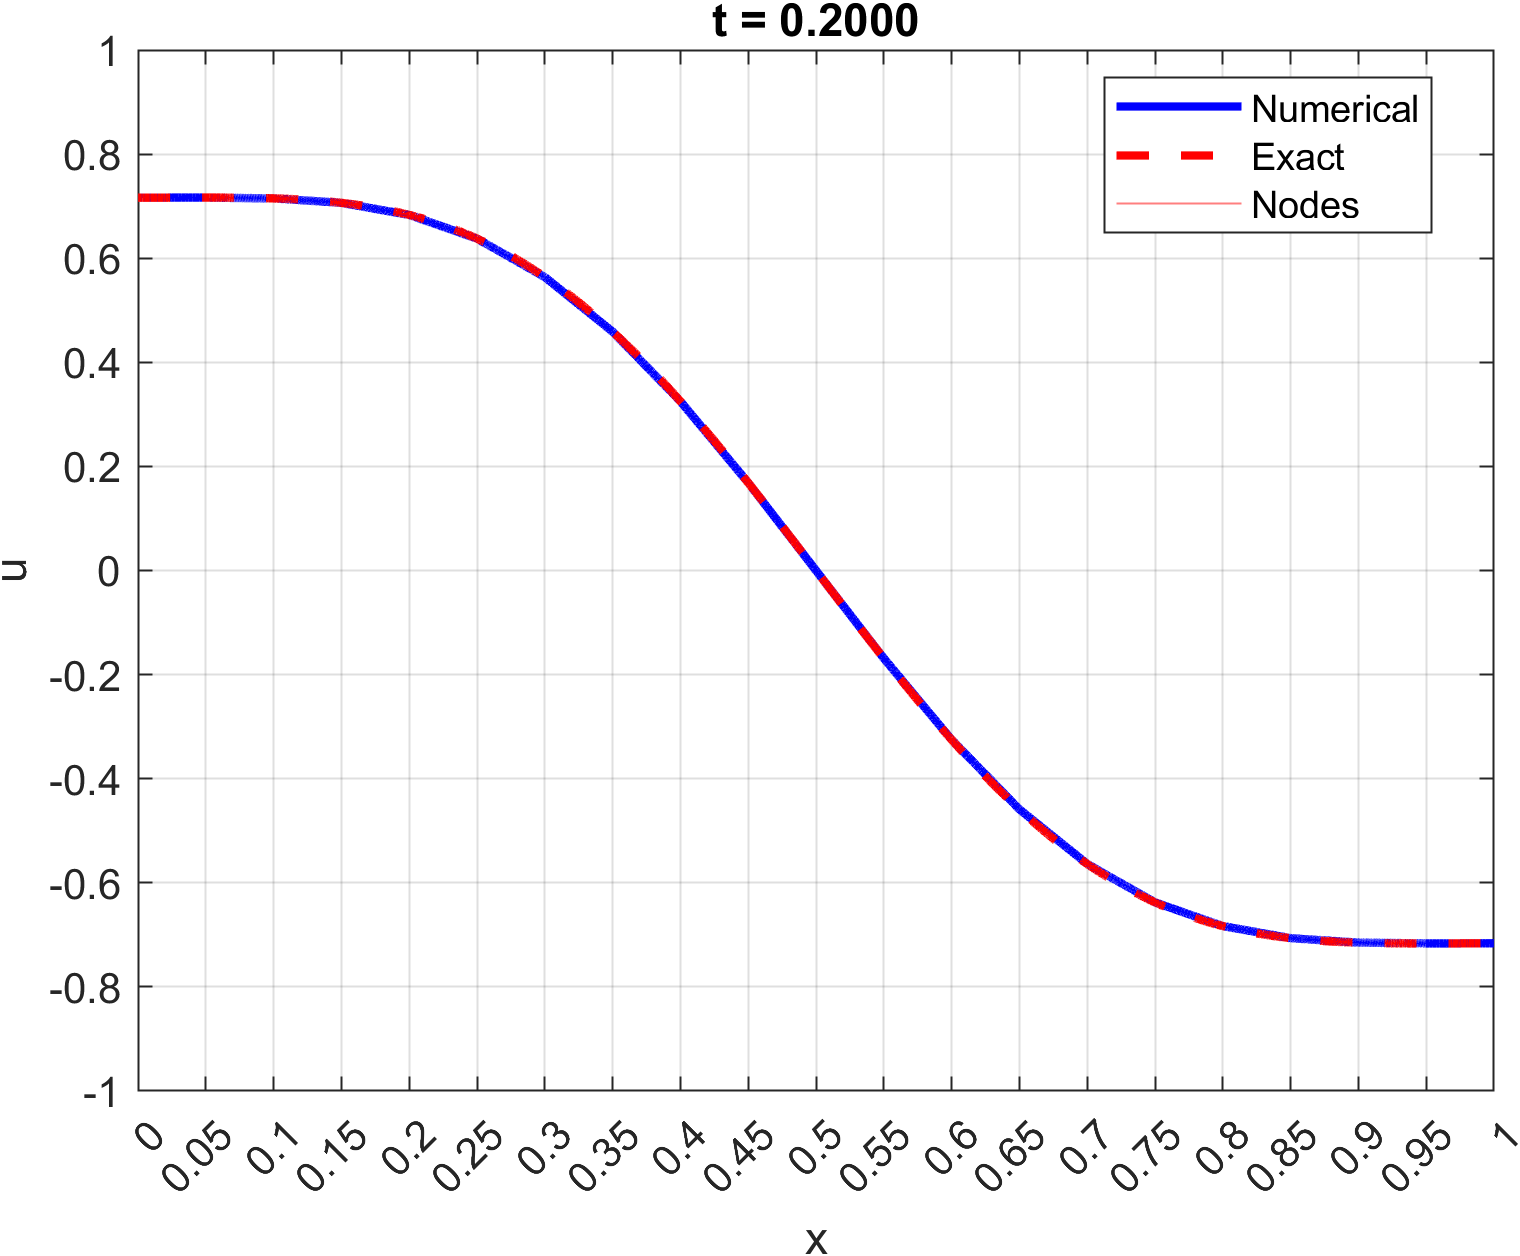
\includegraphics[width=\textwidth]{fdtd_snapshots/experiment_1/snapshot_t_0.2000.png} \caption{FDTD $t=0.2$} \end{subfigure}
    \begin{subfigure}{0.3\textwidth} \centering 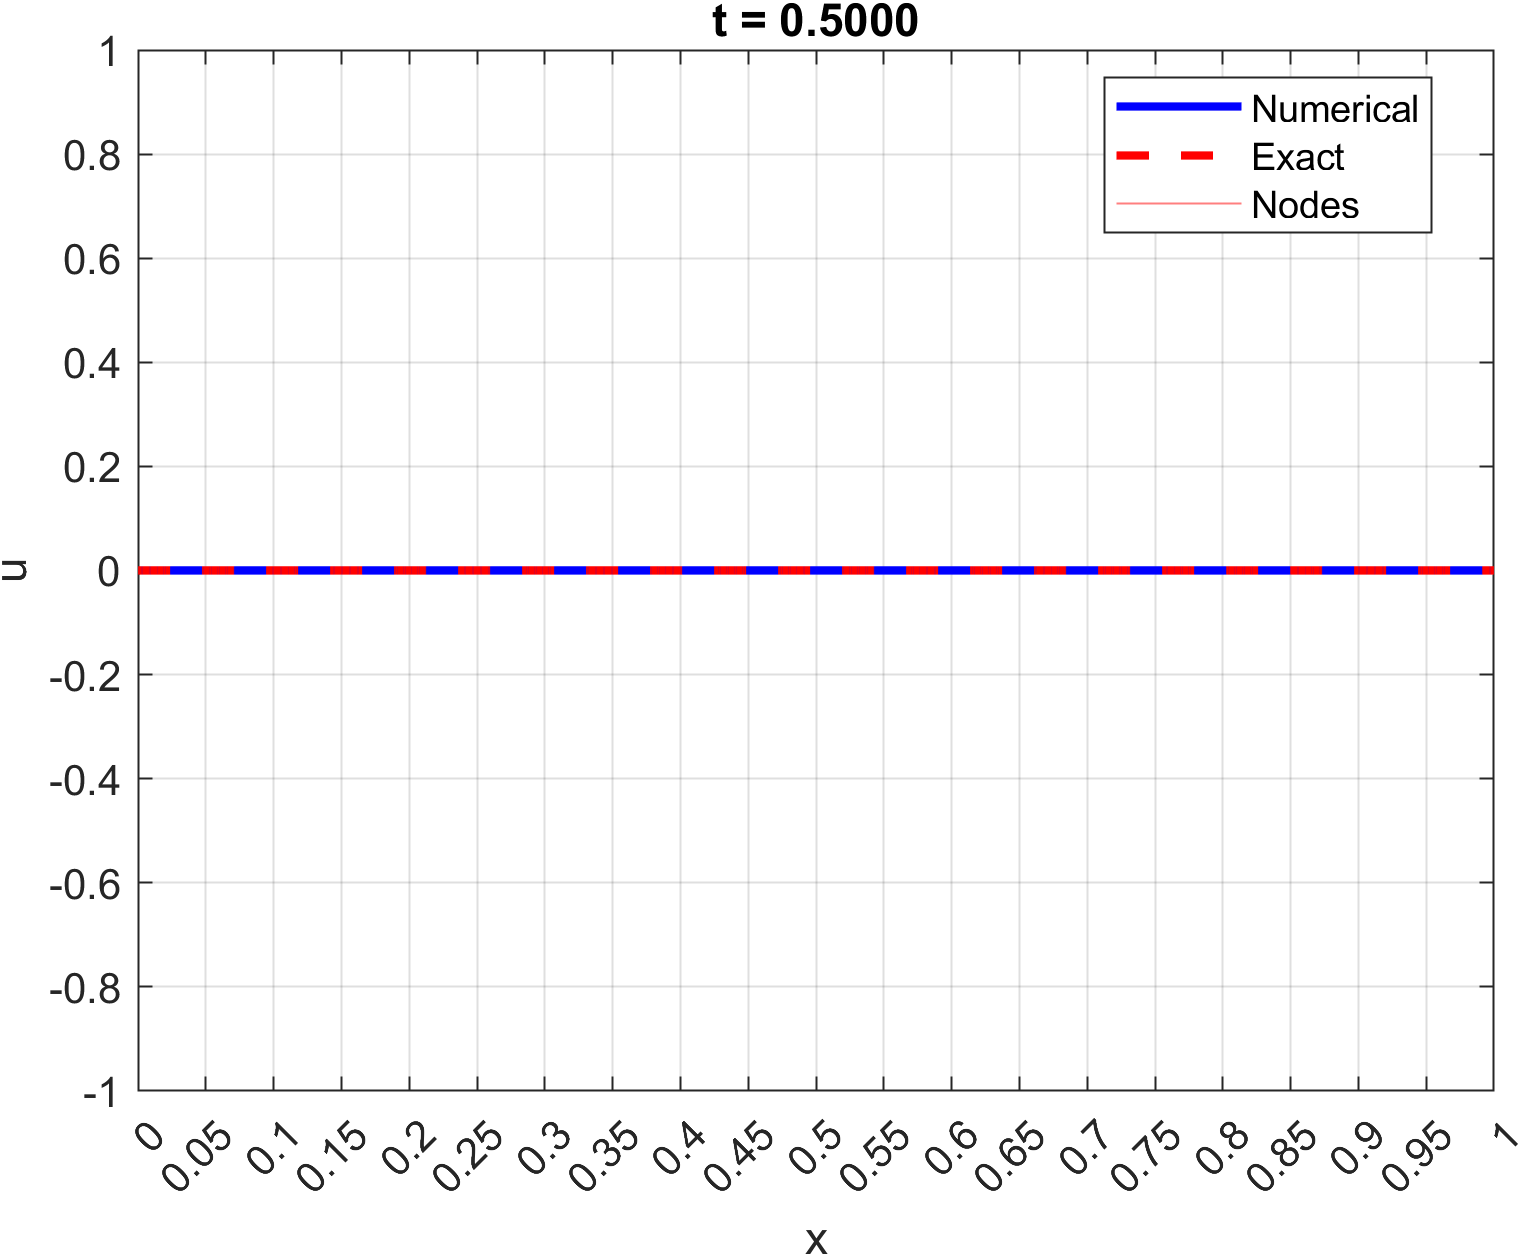
\includegraphics[width=\textwidth]{fdtd_snapshots/experiment_1/snapshot_t_0.5000.png} \caption{FDTD $t=0.5$} \end{subfigure}
    \begin{subfigure}{0.3\textwidth} \centering 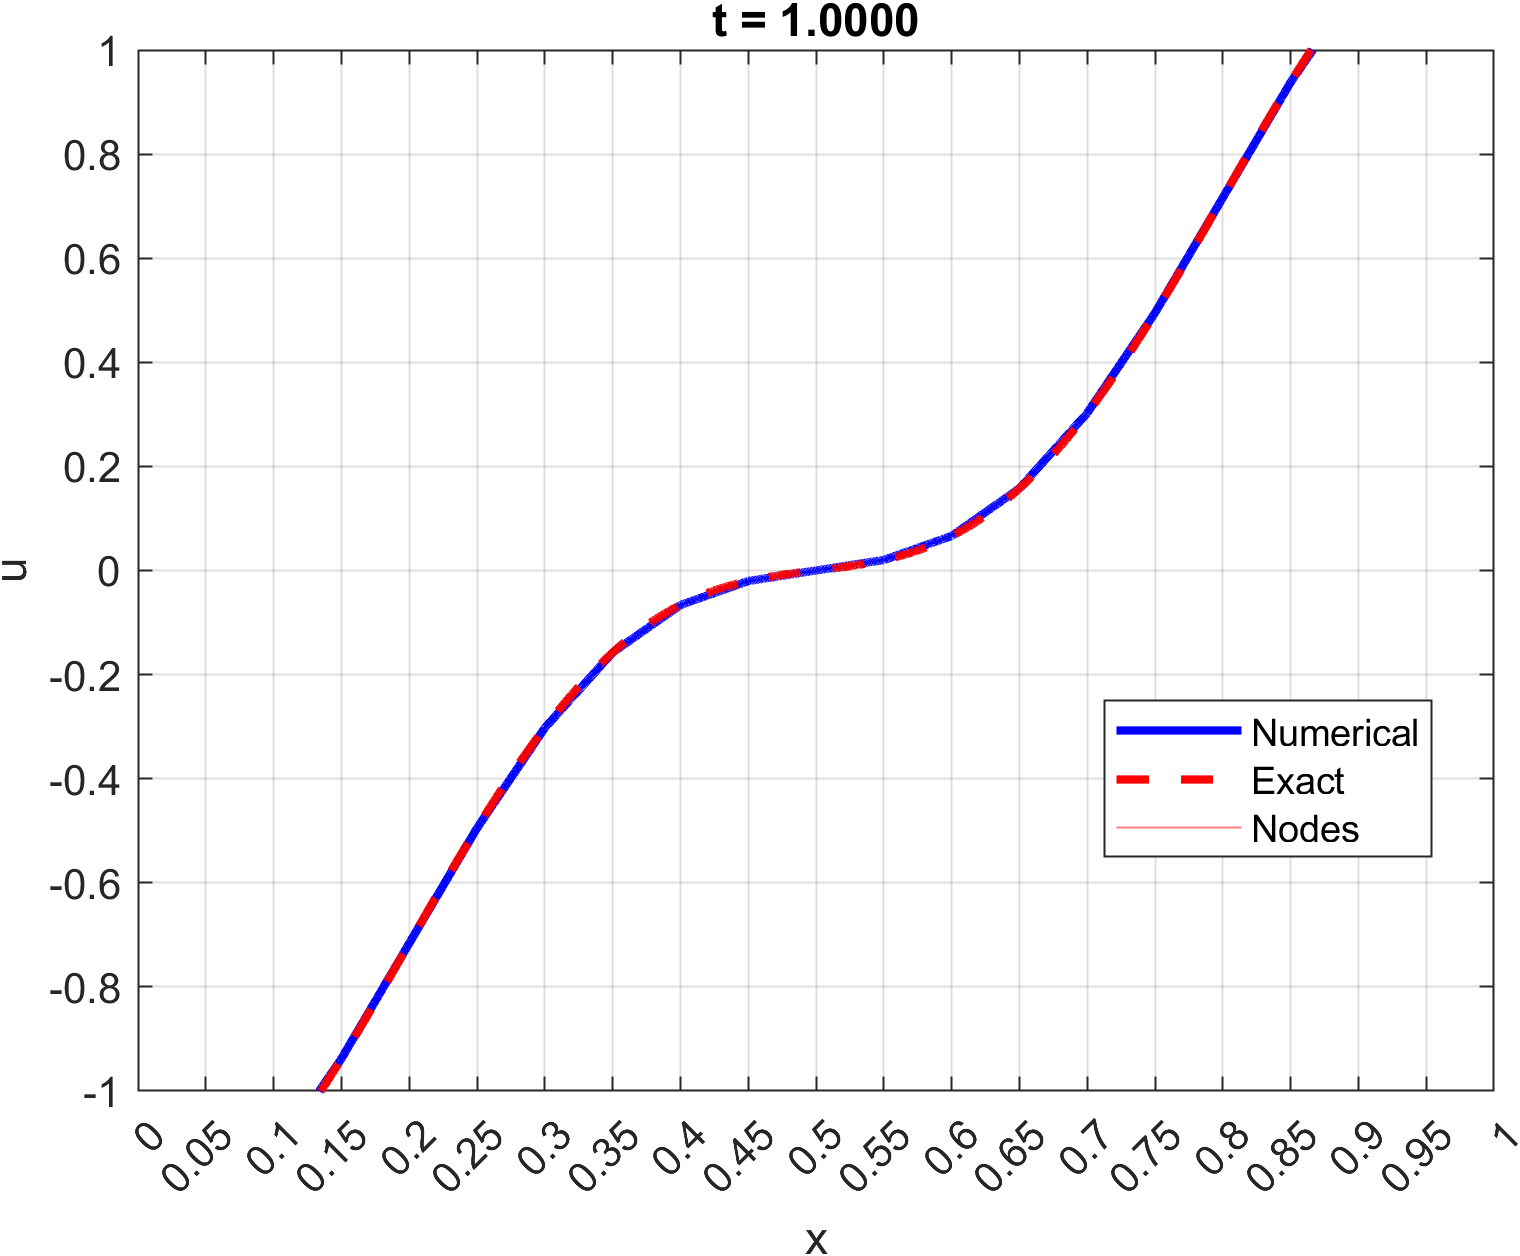
\includegraphics[width=\textwidth]{fdtd_snapshots/experiment_1/snapshot_t_1.0000.png} \caption{FDTD $t=1.0$} \end{subfigure} \\
    \begin{subfigure}{0.3\textwidth} \centering 
\includegraphics[width=\textwidth]{pstd_snapshots/experiment_1/snapshot_t_0.2000.png} \caption{PSTD $t=0.2$} \end{subfigure}
    \begin{subfigure}{0.3\textwidth} \centering 
\includegraphics[width=\textwidth]{pstd_snapshots/experiment_1/snapshot_t_0.5000.png} \caption{PSTD $t=0.5$} \end{subfigure}
    \begin{subfigure}{0.3\textwidth} \centering 
\includegraphics[width=\textwidth]{pstd_snapshots/experiment_1/snapshot_t_1.0000.png} \caption{PSTD $t=1.0$} \end{subfigure}
    \caption{Snapshots of the smooth undamped standing wave.}
\end{figure}

\begin{figure}[H]
    \centering
    \begin{subfigure}{0.48\textwidth} \centering 
\includegraphics[width=\textwidth]{fdtd_snapshots/experiment_1/spacetime_solution.png} \caption{FDTD spacetime.} \end{subfigure}
    \hfill
    \begin{subfigure}{0.48\textwidth} \centering 
\includegraphics[width=\textwidth]{pstd_snapshots/experiment_1/spacetime_solution.png} \caption{PSTD spacetime.} \end{subfigure}
    \caption{Comparison of FDTD and PSTD for smooth undamped standing wave.}
\end{figure}

\begin{figure}[H]
    \centering
    \begin{subfigure}{0.48\textwidth} 
        \centering 
        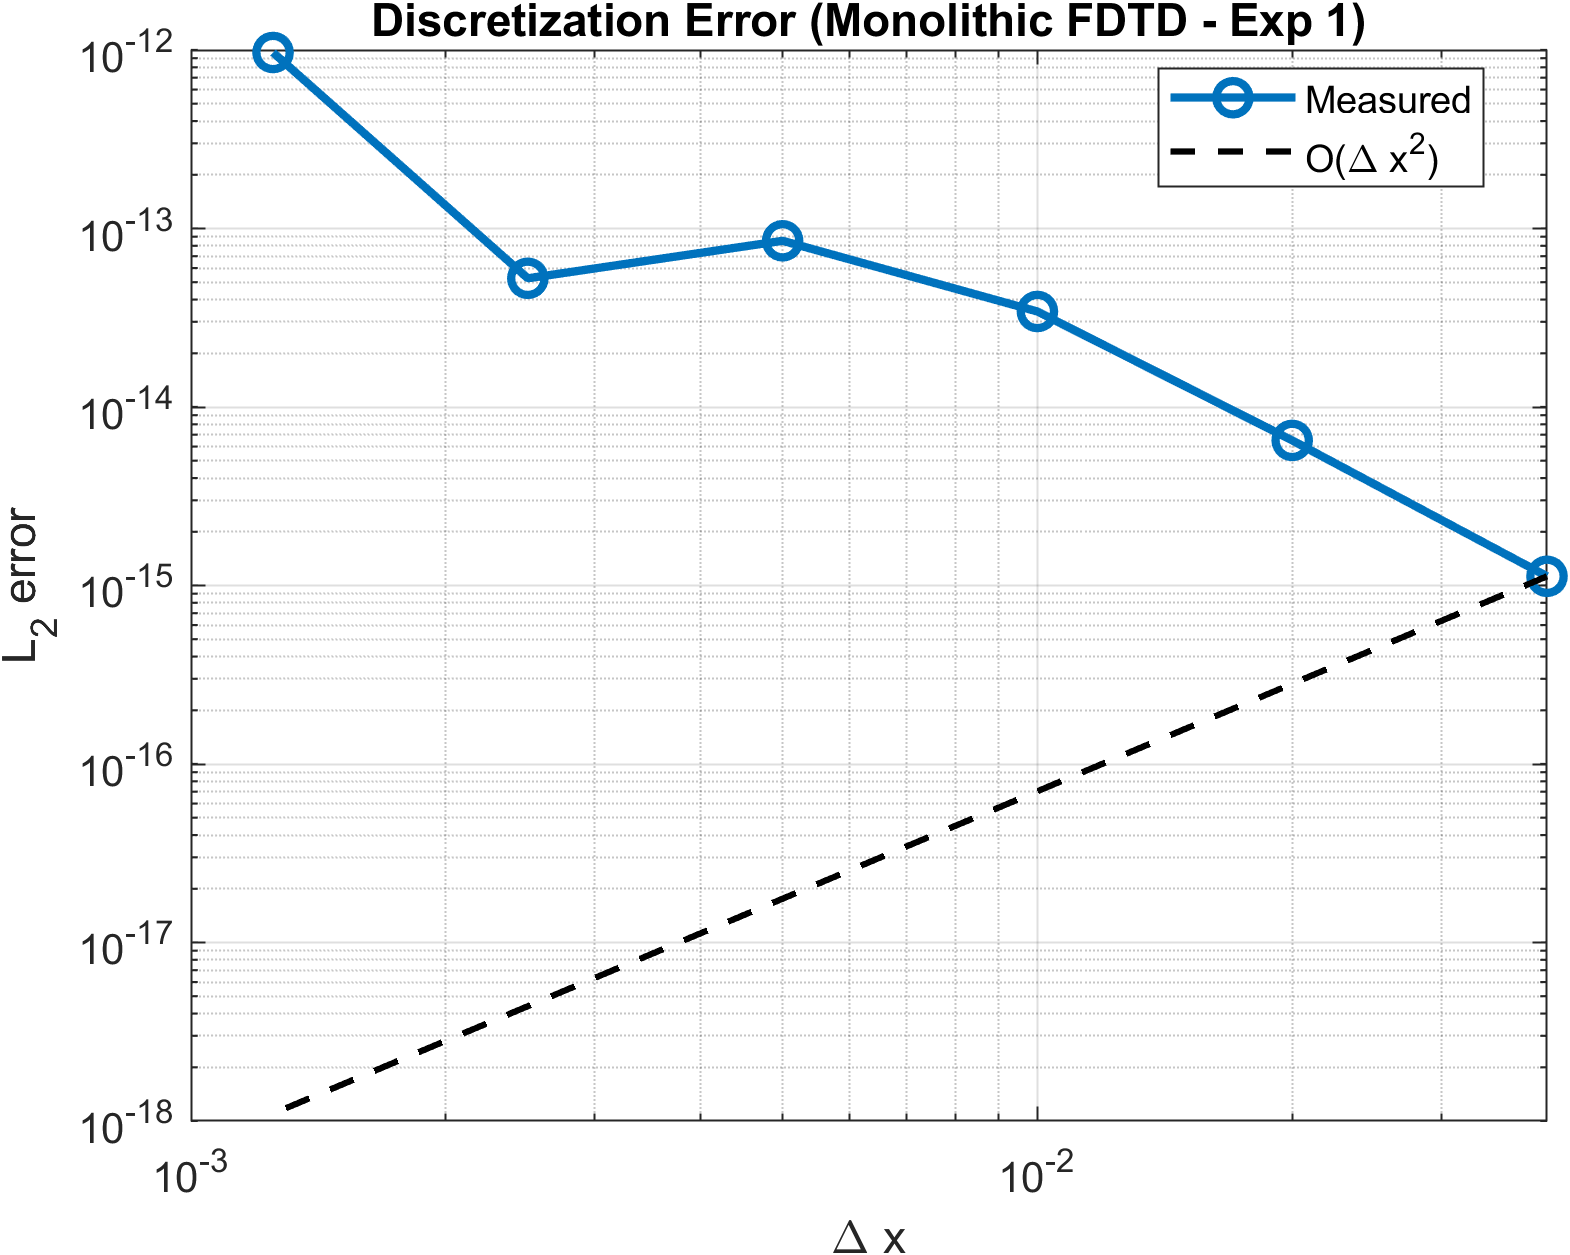
\includegraphics[width=\textwidth]{Images/fdtd_snapshots/experiment_1/final_nodal_error_monolithic.png} 
        \caption{Discretization error (FDTD).} 
    \end{subfigure}
    \hfill
    \begin{subfigure}{0.48\textwidth} 
        \centering 
        
\includegraphics[width=\textwidth]{Images/pstd_snapshots/experiment_1/final_nodal_error_monolithic.png} 
        \caption{Discretization error (PSTD).} 
    \end{subfigure}
    \caption{Convergence analysis for a smooth standing wave. The left column illustrates the FDTD scheme, while the right column shows the PSTD scheme.}
    \label{fig:standing_wave_convergence}
\end{figure}

%%%%%%%%%%%%%%%%%%%%%%%%%%%%%%%%%%%%%%%%%%%%%%%%%%%%%%%%%%%%%%%%%%%%%%%%%%%
\subsection{Non-smooth Standing Wave (Undamped)}

The computational domain, boundary conditions and model parameters are the same as in the previous experiment,
\[
\Omega=(0,L),\qquad
\partial_xu(0,t)=\partial_xu(L,t)=0,\qquad
\gamma=\nu=0.
\]
The initial displacement is a trapezoidal profile, while the initial velocity and forcing vanish,
\[
\partial_tu(x,0)=0,
\qquad
f(x,t)=0.
\]
The reference solution is obtained from the cosine expansion of the initial condition,
\[
u(x,t)
=
\sum_{m=0}^{\infty}
U_m(t)\phi_m(x),
\]
where the modal coefficients are computed analytically from the cosine series and the modal amplitudes evolve according to the exact modal solution. In practice, the series is truncated after a sufficiently large number of modes, making the truncation error negligible. This experiment investigates the effect of reduced spatial regularity on the convergence of the two methods. As in the previous experiment, the FDTD method exhibits the expected exponential convergence of the discretization error. Since the cosine coefficients of non-smooth functions decay algebraically rather than exponentially, the PSTD method exhibits algebraic convergence.

\begin{figure}[H]
    \centering
    \begin{subfigure}{0.3\textwidth} \centering 
\includegraphics[width=\textwidth]{fdtd_snapshots/experiment_2/snapshot_t_0.2000.png} \caption{FDTD $t=0.2$} \end{subfigure}
    \begin{subfigure}{0.3\textwidth} \centering 
\includegraphics[width=\textwidth]{fdtd_snapshots/experiment_2/snapshot_t_0.5000.png} \caption{FDTD $t=0.5$} \end{subfigure}
    \begin{subfigure}{0.3\textwidth} \centering 
\includegraphics[width=\textwidth]{fdtd_snapshots/experiment_2/snapshot_t_1.0000.png} \caption{FDTD $t=1.0$} \end{subfigure} \\
    \begin{subfigure}{0.3\textwidth} \centering 
\includegraphics[width=\textwidth]{pstd_snapshots/experiment_2/snapshot_t_0.2000.png} \caption{PSTD $t=0.2$} \end{subfigure}
    \begin{subfigure}{0.3\textwidth} \centering 
\includegraphics[width=\textwidth]{pstd_snapshots/experiment_2/snapshot_t_0.5000.png} \caption{PSTD $t=0.5$} \end{subfigure}
    \begin{subfigure}{0.3\textwidth} \centering 
\includegraphics[width=\textwidth]{pstd_snapshots/experiment_2/snapshot_t_1.0000.png} \caption{PSTD $t=1.0$} \end{subfigure}
    \caption{Snapshots of the non-smooth undamped standing wave.}
\end{figure}

\begin{figure}[H]
    \centering
    \begin{subfigure}{0.48\textwidth} \centering 
\includegraphics[width=\textwidth]{fdtd_snapshots/experiment_2/spacetime_solution.png} \caption{FDTD spacetime.} \end{subfigure}
    \hfill
    \begin{subfigure}{0.48\textwidth} \centering 
\includegraphics[width=\textwidth]{pstd_snapshots/experiment_2/spacetime_solution.png} \caption{PSTD spacetime.} \end{subfigure}
    \caption{Comparison of FDTD and PSTD for non-smooth undamped standing wave.}
\end{figure}

\begin{figure}[H]
    \centering
    \begin{subfigure}{0.48\textwidth} 
        \centering 
        
\includegraphics[width=\textwidth]{Images/fdtd_snapshots/experiment_2/final_nodal_error_monolithic.png} 
        \caption{Discretization error (FDTD).} 
    \end{subfigure}
    \hfill
    \begin{subfigure}{0.48\textwidth} 
        \centering 
        
\includegraphics[width=\textwidth]{Images/pstd_snapshots/experiment_2/final_nodal_error_monolithic.png} 
        \caption{Discretization error (PSTD).} 
    \end{subfigure}
    \caption{Convergence analysis for a non-smooth standing wave. The left column illustrates the FDTD scheme, while the right column shows the PSTD scheme.}
    \label{fig:nonsmooth_standing_wave_convergence}
\end{figure}

%%%%%%%%%%%%%%%%%%%%%%%%%%%%%%%%%%%%%%%%%%%%%%%%%%%%%%%%%%%%%%%%%%%%%%%%%%%
\subsection{Smooth Standing Wave (Damped)}

The computational domain is $\Omega=(0,L)$ with homogeneous Neumann boundary conditions,
\[
\partial_xu(0,t)=\partial_xu(L,t)=0.
\]
The damping coefficients are chosen as
\[
\gamma=0.5,
\qquad
\nu=0.005.
\]
The initial displacement is identical to that of the first experiment,
\[
u(x,0)
=
\cos\!\left(\frac{\pi x}{L}\right)
+
0.3\cos\!\left(\frac{3\pi x}{L}\right),
\]
with
\[
\partial_tu(x,0)=0,
\qquad
f(x,t)=0.
\]
The exact solution is again obtained through the analytical modal evolution,
\[
u(x,t)
=
\sum_{m\in\{1,3\}}
U_m(t)\phi_m(x),
\]
where the modal amplitudes now include the effect of telegrapher and viscoelastic damping. This benchmark assesses the accuracy of the schemes for smooth damped standing waves. The FDTD method exhibits the expected second-order convergence of the discretization error. Since the exact solution is completely represented by the retained cosine modes, the PSTD method reproduces the solution up to machine precision.

\begin{figure}[H]
    \centering
    \begin{subfigure}{0.3\textwidth} \centering 
\includegraphics[width=\textwidth]{fdtd_snapshots/experiment_3/snapshot_t_0.2000.png} \caption{FDTD $t=0.2$} \end{subfigure}
    \begin{subfigure}{0.3\textwidth} \centering 
\includegraphics[width=\textwidth]{fdtd_snapshots/experiment_3/snapshot_t_0.5000.png} \caption{FDTD $t=0.5$} \end{subfigure}
    \begin{subfigure}{0.3\textwidth} \centering 
\includegraphics[width=\textwidth]{fdtd_snapshots/experiment_3/snapshot_t_1.0000.png} \caption{FDTD $t=1.0$} \end{subfigure} \\
    \begin{subfigure}{0.3\textwidth} \centering 
\includegraphics[width=\textwidth]{pstd_snapshots/experiment_3/snapshot_t_0.2000.png} \caption{PSTD $t=0.2$} \end{subfigure}
    \begin{subfigure}{0.3\textwidth} \centering 
\includegraphics[width=\textwidth]{pstd_snapshots/experiment_3/snapshot_t_0.5000.png} \caption{PSTD $t=0.5$} \end{subfigure}
    \begin{subfigure}{0.3\textwidth} \centering 
\includegraphics[width=\textwidth]{pstd_snapshots/experiment_3/snapshot_t_1.0000.png} \caption{PSTD $t=1.0$} \end{subfigure}
    \caption{Snapshots of the smooth damped standing wave.}
\end{figure}

\begin{figure}[H]
    \centering
    \begin{subfigure}{0.48\textwidth} \centering 
\includegraphics[width=\textwidth]{fdtd_snapshots/experiment_3/spacetime_solution.png} \caption{FDTD spacetime.} \end{subfigure}
    \hfill
    \begin{subfigure}{0.48\textwidth} \centering 
\includegraphics[width=\textwidth]{pstd_snapshots/experiment_3/spacetime_solution.png} \caption{PSTD spacetime.} \end{subfigure}
    \caption{Comparison of FDTD and PSTD for smooth damped standing wave.}
\end{figure}

\begin{figure}[H]
    \centering
    \begin{subfigure}{0.48\textwidth} 
        \centering 
        
\includegraphics[width=\textwidth]{Images/fdtd_snapshots/experiment_3/final_nodal_error_monolithic.png} 
        \caption{Discretization error (FDTD).} 
    \end{subfigure}
    \hfill
    \begin{subfigure}{0.48\textwidth} 
        \centering 
        
\includegraphics[width=\textwidth]{Images/pstd_snapshots/experiment_3/final_nodal_error_monolithic.png} 
        \caption{Discretization error (PSTD).} 
    \end{subfigure}
    \caption{Convergence analysis for a non-smooth standing wave with damping. The left column illustrates the FDTD scheme, while the right column shows the PSTD scheme.}
    \label{fig:nonsmooth_damped_standing_wave_convergence}
\end{figure}

%%%%%%%%%%%%%%%%%%%%%%%%%%%%%%%%%%%%%%%%%%%%%%%%%%%%%%%%%%%%%%%%%%%%%%%%%%%
\subsection{Non-smooth Standing Wave (Damped)}

The computational domain, boundary conditions and damping parameters are the same as in the previous experiment,
\[
\Omega=(0,L),\qquad
\partial_xu(0,t)=\partial_xu(L,t)=0,
\]
with
\[
\gamma=0.5,
\qquad
\nu=0.005.
\]
The initial displacement is the same trapezoidal profile considered in the second experiment, while
\[
\partial_tu(x,0)=0,
\qquad
f(x,t)=0.
\]
The reference solution is computed from the cosine expansion of the initial condition, with each modal coefficient propagated analytically according to the damped modal dynamics. As in the undamped case, the modal expansion is truncated after a sufficiently large number of modes. This benchmark investigates the influence of damping on non-smooth initial data. The FDTD method is expected to retain second-order convergence of the truncation error. However, the limited spatial regularity of the initial profile introduces an initial error that propagates and cannot be completely distinguished from the discretization error, resulting in an observed convergence rate slightly below second order. For the PSTD method, the discretization error continues to converge algebraically.

\begin{figure}[H]
    \centering
    \begin{subfigure}{0.3\textwidth} \centering 
\includegraphics[width=\textwidth]{fdtd_snapshots/experiment_4/snapshot_t_0.2000.png} \caption{FDTD $t=0.2$} \end{subfigure}
    \begin{subfigure}{0.3\textwidth} \centering 
\includegraphics[width=\textwidth]{fdtd_snapshots/experiment_4/snapshot_t_0.5000.png} \caption{FDTD $t=0.5$} \end{subfigure}
    \begin{subfigure}{0.3\textwidth} \centering 
\includegraphics[width=\textwidth]{fdtd_snapshots/experiment_4/snapshot_t_1.0000.png} \caption{FDTD $t=1.0$} \end{subfigure} \\
    \begin{subfigure}{0.3\textwidth} \centering 
\includegraphics[width=\textwidth]{pstd_snapshots/experiment_4/snapshot_t_0.2000.png} \caption{PSTD $t=0.2$} \end{subfigure}
    \begin{subfigure}{0.3\textwidth} \centering 
\includegraphics[width=\textwidth]{pstd_snapshots/experiment_4/snapshot_t_0.5000.png} \caption{PSTD $t=0.5$} \end{subfigure}
    \begin{subfigure}{0.3\textwidth} \centering 
\includegraphics[width=\textwidth]{pstd_snapshots/experiment_4/snapshot_t_1.0000.png} \caption{PSTD $t=1.0$} \end{subfigure}
    \caption{Snapshots of the non-smooth damped standing wave.}
\end{figure}

\begin{figure}[H]
    \centering
    \begin{subfigure}{0.48\textwidth} \centering 
\includegraphics[width=\textwidth]{fdtd_snapshots/experiment_4/spacetime_solution.png} \caption{FDTD spacetime.} \end{subfigure}
    \hfill
    \begin{subfigure}{0.48\textwidth} \centering 
\includegraphics[width=\textwidth]{pstd_snapshots/experiment_4/spacetime_solution.png} \caption{PSTD spacetime.} \end{subfigure}
    \caption{Comparison of FDTD and PSTD for non-smooth damped standing wave.}
\end{figure}

\begin{figure}[H]
    \centering
    \begin{subfigure}{0.48\textwidth} 
        \centering 
        
\includegraphics[width=\textwidth]{Images/fdtd_snapshots/experiment_4/final_nodal_error_monolithic.png} 
        \caption{Discretization error (FDTD).} 
    \end{subfigure}
    \hfill
    \begin{subfigure}{0.48\textwidth} 
        \centering 
        
\includegraphics[width=\textwidth]{Images/pstd_snapshots/experiment_4/final_nodal_error_monolithic.png} 
        \caption{Discretization error (PSTD).} 
    \end{subfigure}
    \caption{Convergence analysis for a non-smooth standing wave with damping (Experiment 4). The left column illustrates the FDTD scheme, while the right column shows the PSTD scheme.}
    \label{fig:experiment_4_convergence}
\end{figure}

%%%%%%%%%%%%%%%%%%%%%%%%%%%%%%%%%%%%%%%%%%%%%%%%%%%%%%%%%%%%%%%%%%%%%%%%%%%
\subsection{Smooth Propagating Waves (Undamped)}

The computational domain is $\Omega=(0,L)$ and homogeneous Neumann boundary conditions are imposed,
\[
\partial_xu(0,t)=\partial_xu(L,t)=0.
\]
The damping coefficients are
\[
\gamma=\nu=0.
\]
The initial displacement is a Gaussian pulse centered at
\[
\mu=\frac{L}{4},
\]
with width parameter $\sigma=L/50$,
\[
u(x,0)
=
\exp\!\left(
-\frac{(x-\mu)^2}{2\sigma^2}
\right),
\]
while
\[
\partial_tu(x,0)=0,
\qquad
f(x,t)=0.
\]

The reference solution is obtained by combining the classical d'Alembert formula with the method of images. More precisely, the initial condition is extended to an even $2L$-periodic function,
\[
u_0^{\mathrm{ext}}(x),
\]
which automatically satisfies the homogeneous Neumann boundary conditions. The exact solution is therefore
\[
u(x,t)
=
\frac12
u_0^{\mathrm{ext}}(x-ct)
+
\frac12
u_0^{\mathrm{ext}}(x+ct).
\]
Equivalently, the solution can be interpreted as the superposition of the original pulse together with an infinite family of virtual image sources located at
\[
x=2mL\pm\mu,
\qquad
m\in\mathbb Z,
\]
whose reflections preserve the sign of the wave. This construction exactly reproduces the multiple reflections occurring at the Neumann boundaries. This experiment evaluates the propagation accuracy of the two schemes under repeated Neumann reflections. As in Experiment~1, the FDTD method exhibits the expected exponential convergence of the discretization error. Although the Gaussian pulse is not exactly represented by a finite cosine expansion, its cosine coefficients decay exponentially. Consequently, the PSTD method rapidly reaches machine precision.

\begin{figure}[H]
    \centering
    \begin{subfigure}{0.3\textwidth} \centering 
\includegraphics[width=\textwidth]{fdtd_snapshots/experiment_5/snapshot_t_0.2000.png} \caption{FDTD $t=0.2$} \end{subfigure}
    \begin{subfigure}{0.3\textwidth} \centering 
\includegraphics[width=\textwidth]{fdtd_snapshots/experiment_5/snapshot_t_0.5000.png} \caption{FDTD $t=0.5$} \end{subfigure}
    \begin{subfigure}{0.3\textwidth} \centering 
\includegraphics[width=\textwidth]{fdtd_snapshots/experiment_5/snapshot_t_1.0000.png} \caption{FDTD $t=1.0$} \end{subfigure} \\
    \begin{subfigure}{0.3\textwidth} \centering 
\includegraphics[width=\textwidth]{pstd_snapshots/experiment_5/snapshot_t_0.2000.png} \caption{PSTD $t=0.2$} \end{subfigure}
    \begin{subfigure}{0.3\textwidth} \centering 
\includegraphics[width=\textwidth]{pstd_snapshots/experiment_5/snapshot_t_0.5000.png} \caption{PSTD $t=0.5$} \end{subfigure}
    \begin{subfigure}{0.3\textwidth} \centering 
\includegraphics[width=\textwidth]{pstd_snapshots/experiment_5/snapshot_t_1.0000.png} \caption{PSTD $t=1.0$} \end{subfigure}
    \caption{Snapshots of the Gaussian pulse.}
\end{figure}

\begin{figure}[H]
    \centering
    \begin{subfigure}{0.48\textwidth} \centering 
\includegraphics[width=\textwidth]{fdtd_snapshots/experiment_5/spacetime_solution.png} \caption{FDTD spacetime.} \end{subfigure}
    \hfill
    \begin{subfigure}{0.48\textwidth} \centering 
\includegraphics[width=\textwidth]{pstd_snapshots/experiment_5/spacetime_solution.png} \caption{PSTD spacetime.} \end{subfigure}
    \caption{Comparison of FDTD and PSTD for propagating Gaussian pulse.}
\end{figure}

\begin{figure}[H]
    \centering
    \begin{subfigure}{0.48\textwidth} 
        \centering 
        
\includegraphics[width=\textwidth]{Images/fdtd_snapshots/experiment_5/final_nodal_error_monolithic.png} 
        \caption{Discretization error (FDTD).} 
    \end{subfigure}
    \hfill
    \begin{subfigure}{0.48\textwidth} 
        \centering 
        
\includegraphics[width=\textwidth]{Images/pstd_snapshots/experiment_5/final_nodal_error_monolithic.png} 
        \caption{Discretization error (PSTD).} 
    \end{subfigure}
    \caption{Convergence analysis for smooth propagating waves (Experiment 5). The left column illustrates the FDTD scheme, while the right column shows the PSTD scheme.}
    \label{fig:experiment_5_convergence}
\end{figure}

%%%%%%%%%%%%%%%%%%%%%%%%%%%%%%%%%%%%%%%%%%%%%%%%%%%%%%%%%%%%%%%%%%%%%%%%%%%
\subsection{Non-smooth Propagating Waves (Undamped)}

The computational domain, boundary conditions and physical parameters coincide with those of the previous experiment,
\[
\Omega=(0,L),\qquad
\partial_xu(0,t)=\partial_xu(L,t)=0,\qquad
\gamma=\nu=0.
\]
The initial displacement is a triangular pulse centered at
\[
\mu=\frac{L}{4},
\]
with support determined by $\sigma=L/50$, while
\[
\partial_tu(x,0)=0,
\qquad
f(x,t)=0.
\]

As in the previous experiment, the reference solution is obtained by combining the classical d'Alembert formula with the method of images. The initial triangular profile is extended to an even $2L$-periodic function,
\[
u_0^{\mathrm{ext}}(x),
\]
yielding the exact solution
\[
u(x,t)
=
\frac12
u_0^{\mathrm{ext}}(x-ct)
+
\frac12
u_0^{\mathrm{ext}}(x+ct).
\]
Equivalently, the solution may be viewed as the superposition of the original triangular pulse and an infinite family of virtual image sources located at
\[
x=2mL\pm\mu,
\qquad
m\in\mathbb Z,
\]
whose reflections preserve the sign of the wave. This construction exactly reproduces the multiple reflections induced by the homogeneous Neumann boundary conditions. This benchmark evaluates the behavior of the two methods for propagating solutions with limited spatial regularity and sharp gradients. The FDTD method again exhibits the expected exponential convergence of the discretization error. Since the solution is non-smooth, the cosine coefficients decay only algebraically, leading the PSTD method to exhibit algebraic convergence.

\begin{figure}[H]
    \centering
    \begin{subfigure}{0.3\textwidth} \centering 
\includegraphics[width=\textwidth]{fdtd_snapshots/experiment_6/snapshot_t_0.2000.png} \caption{FDTD $t=0.2$} \end{subfigure}
    \begin{subfigure}{0.3\textwidth} \centering 
\includegraphics[width=\textwidth]{fdtd_snapshots/experiment_6/snapshot_t_0.5000.png} \caption{FDTD $t=0.5$} \end{subfigure}
    \begin{subfigure}{0.3\textwidth} \centering 
\includegraphics[width=\textwidth]{fdtd_snapshots/experiment_6/snapshot_t_1.0000.png} \caption{FDTD $t=1.0$} \end{subfigure} \\
    \begin{subfigure}{0.3\textwidth} \centering 
\includegraphics[width=\textwidth]{pstd_snapshots/experiment_6/snapshot_t_0.2000.png} \caption{PSTD $t=0.2$} \end{subfigure}
    \begin{subfigure}{0.3\textwidth} \centering 
\includegraphics[width=\textwidth]{pstd_snapshots/experiment_6/snapshot_t_0.5000.png} \caption{PSTD $t=0.5$} \end{subfigure}
    \begin{subfigure}{0.3\textwidth} \centering 
\includegraphics[width=\textwidth]{pstd_snapshots/experiment_6/snapshot_t_1.0000.png} \caption{PSTD $t=1.0$} \end{subfigure}
    \caption{Snapshots of the triangular pulse.}
\end{figure}

\begin{figure}[H]
    \centering
    \begin{subfigure}{0.48\textwidth} \centering 
\includegraphics[width=\textwidth]{fdtd_snapshots/experiment_6/spacetime_solution.png} \caption{FDTD spacetime.} \end{subfigure}
    \hfill
    \begin{subfigure}{0.48\textwidth} \centering 
\includegraphics[width=\textwidth]{pstd_snapshots/experiment_6/spacetime_solution.png} \caption{PSTD spacetime.} \end{subfigure}
    \caption{Comparison of FDTD and PSTD for propagating triangular pulse.}
\end{figure}

\begin{figure}[H]
    \centering
    \begin{subfigure}{0.48\textwidth} 
        \centering 
        
\includegraphics[width=\textwidth]{Images/fdtd_snapshots/experiment_6/final_nodal_error_monolithic.png} 
        \caption{Discretization error (FDTD).} 
    \end{subfigure}
    \hfill
    \begin{subfigure}{0.48\textwidth} 
        \centering 
        
\includegraphics[width=\textwidth]{Images/pstd_snapshots/experiment_6/final_nodal_error_monolithic.png} 
        \caption{Discretization error (PSTD).} 
    \end{subfigure}
    \caption{Convergence analysis for non-smooth propagating waves (Experiment 6). The left column illustrates the FDTD scheme, while the right column shows the PSTD scheme.}
    \label{fig:experiment_6_convergence}
\end{figure}

\chapter{Acceleration of the Numerical Solvers and Inverse Problems}

\section{Optimized Schwarz Waveform Relaxation}

To solve the damped wave equation on large computational domains, we employ an overlapping Schwarz Waveform Relaxation (SWR) method. For the classical Schwarz Waveform Relaxation method, Dirichlet transmission conditions are employed, whereas for Optimized Schwarz Waveform Relaxation (OSWR) methods, we develop transmission operators that minimize the convergence factor. We employ Robin-like transmission conditions depending on two parameters $q$ and $r$. As the PSTD method only supports homogeneous Neumann conditions, we employ SWR only for FDTD.

\subsection{Algorithm}
Let
\[
\Omega=(0,L)
\]
be decomposed into the two overlapping subdomains
\[
\Omega_1=(0,b),
\qquad
\Omega_2=(a,L),
\]
with
\[
0<a<b<L,
\qquad
\delta=b-a>0,
\]
where $\delta$ denotes the overlap width.

At Schwarz iteration $k+1$, the subdomain problems are

\begin{align}
u_{tt}^{(k+1)}
+\gamma u_t^{(k+1)}
&=
c^2u_{xx}^{(k+1)}
+\nu u_{xxt}^{(k+1)}
+f,
&&x\in(0,b),
\\
v_{tt}^{(k+1)}
+\gamma v_t^{(k+1)}
&=
c^2v_{xx}^{(k+1)}
+\nu v_{xxt}^{(k+1)}
+f,
&&x\in(a,L),
\end{align}

subject to the physical boundary conditions at $x=0$ and $x=L$, together with Robin transmission conditions at the interfaces

\begin{align}
u_x^{(k+1)}(b,t)
+
q\,u_t^{(k+1)}(b,t)
+
r\,u^{(k+1)}(b,t)
&=
v_x^{(k)}(b,t)
+
q\,v_t^{(k)}(b,t)
+
r\,v^{(k)}(b,t),
\\
-v_x^{(k+1)}(a,t)
+
q\,v_t^{(k+1)}(a,t)
+
r\,v^{(k+1)}(a,t)
&=
-u_x^{(k)}(a,t)
+
q\,u_t^{(k)}(a,t)
+
r\,u^{(k)}(a,t).
\end{align}

The symbols $q,r\ge0$ are the transmission operator parameters that we want to optimize.

\subsection{Convergence Factor}

To analyze the convergence of the algorithm, it is sufficient to consider the error equations. Since the exact solution satisfies the same equations, the forcing term, initial conditions and physical boundary data vanish. We therefore study

\begin{equation}
u_{tt}
+\gamma u_t
=
c^2u_{xx}
+\nu u_{xxt},
\end{equation}

with homogeneous Neumann boundary conditions.

Applying the Laplace transform in time gives

\begin{equation}
(c^2+\nu s)\widehat{u}_{xx}
=
(s^2+\gamma s)\widehat{u}.
\end{equation}

Introducing the Laplace-domain wavenumber

\begin{equation}
k(s)
=
\sqrt{
\frac{-s^2-\gamma s}
     {c^2+\nu s}
},
\label{eq:kappa_laplace}
\end{equation}

the transformed equation becomes

\begin{equation}
\widehat{u}_{xx}
+
k(s)^2
\widehat{u}
=
0.
\end{equation}

Restricting the Laplace variable to the imaginary axis,
\[
s=i\omega,
\]
recovers the continuous dispersion relation derived in
Section~\ref{sec:dispersion_analysis}, since
\[
k(i\omega)
=
\sqrt{
\frac{\omega^2-i\gamma\omega}
     {c^2+i\nu\omega}
}.
\]

The Laplace symbol of the Robin operator is

\begin{equation}
\Lambda(s)=qs+r.
\end{equation}

The homogeneous Neumann conditions at the physical boundaries constrain the general exponential solutions of
\[
\widehat{u}_{xx}+k^2\widehat{u}=0,
\qquad
\widehat{v}_{xx}+k^2\widehat{v}=0
\]
on each subdomain. Writing the general solution as a superposition of counter-propagating exponentials,
\begin{align}
\widehat{u}(x,s) &= \alpha_u\,e^{ikx} + \beta_u\,e^{-ikx}, \\
\widehat{v}(x,s) &= \alpha_v\,e^{ik(L-x)} + \beta_v\,e^{-ik(L-x)},
\end{align}
with derivatives
\[
\widehat{u}_x(x,s) = ik\left(\alpha_u e^{ikx}-\beta_u e^{-ikx}\right),
\qquad
\widehat{v}_x(x,s) = -ik\left(\alpha_v e^{ik(L-x)}-\beta_v e^{-ik(L-x)}\right).
\]
Imposing $\widehat u_x(0,s)=0$, $\widehat v_x(L,s)=0$ forces $\beta_u=\alpha_u$ and $\beta_v=\alpha_v$. Absorbing the amplitude into a single constant on each subdomain gives

\begin{align}
\widehat{u}(x,s) &= A_u\left(e^{ikx}+e^{-ikx}\right), \\
\widehat{v}(x,s) &= A_v\left(e^{ik(L-x)}+e^{-ik(L-x)}\right),
\end{align}

with corresponding derivatives

\begin{align}
\widehat{u}_x(x,s) &= ikA_u\left(e^{ikx}-e^{-ikx}\right), \\
\widehat{v}_x(x,s) &= -ikA_v\left(e^{ik(L-x)}-e^{-ik(L-x)}\right).
\end{align}

Using $L-a=b$ and $L-b=a$, the interface traces are

\begin{align}
\widehat{u}(a) &= A_u\left(e^{ika}+e^{-ika}\right),
&
\widehat{u}_x(a) &= ikA_u\left(e^{ika}-e^{-ika}\right),
\\
\widehat{u}(b) &= A_u\left(e^{ikb}+e^{-ikb}\right),
&
\widehat{u}_x(b) &= ikA_u\left(e^{ikb}-e^{-ikb}\right),
\\
\widehat{v}(a) &= A_v\left(e^{ikb}+e^{-ikb}\right),
&
\widehat{v}_x(a) &= -ikA_v\left(e^{ikb}-e^{-ikb}\right),
\\
\widehat{v}(b) &= A_v\left(e^{ika}+e^{-ika}\right),
&
\widehat{v}_x(b) &= -ikA_v\left(e^{ika}-e^{-ika}\right).
\end{align}

Substituting into the Laplace-transformed Robin transmission conditions,

\begin{align}
(\partial_x+\Lambda)\widehat{u}^{(k+1)}(b)
&=
(\partial_x+\Lambda)\widehat{v}^{(k)}(b),
\\
(-\partial_x+\Lambda)\widehat{v}^{(k+1)}(a)
&=
(-\partial_x+\Lambda)\widehat{u}^{(k)}(a),
\end{align}

gives

\begin{align}
A_u^{(k+1)}
\Bigl[
ik\left(e^{ikb}-e^{-ikb}\right)
+\Lambda\left(e^{ikb}+e^{-ikb}\right)
\Bigr]
&=
A_v^{(k)}
\Bigl[
-ik\left(e^{ika}-e^{-ika}\right)
+\Lambda\left(e^{ika}+e^{-ika}\right)
\Bigr],
\\
A_v^{(k+1)}
\Bigl[
ik\left(e^{ikb}-e^{-ikb}\right)
+\Lambda\left(e^{ikb}+e^{-ikb}\right)
\Bigr]
&=
A_u^{(k)}
\Bigl[
-ik\left(e^{ika}-e^{-ika}\right)
+\Lambda\left(e^{ika}+e^{-ika}\right)
\Bigr].
\end{align}

Denoting the bracketed quantities by
\[
F(b) = ik\left(e^{ikb}-e^{-ikb}\right)+\Lambda\left(e^{ikb}+e^{-ikb}\right),
\qquad
H(a) = -ik\left(e^{ika}-e^{-ika}\right)+\Lambda\left(e^{ika}+e^{-ika}\right),
\]
the two equations decouple into a two-step recurrence
\begin{equation}
A_u^{(k+2)} = G(s)^2 A_u^{(k)},
\qquad
G(s) = \frac{H(a)}{F(b)}.
\end{equation}

We now pass from exponentials to hyperbolic functions using
\[
e^{ikz}-e^{-ikz}=2\sinh(ikz),
\qquad
e^{ikz}+e^{-ikz}=2\cosh(ikz),
\]
which gives
\begin{align}
F(b) &= 2\left[ik\sinh(ikb)+\Lambda\cosh(ikb)\right], \\
H(a) &= 2\left[-ik\sinh(ika)+\Lambda\cosh(ika)\right].
\end{align}

Hence, the convergence factor is

\begin{equation}
\rho(s)
=
|G(s)|
=
\left|
\frac{
ik(s)\sinh\bigl(ik(s)a\bigr)
-
\Lambda(s)\cosh\bigl(ik(s)a\bigr)
}{
ik(s)\sinh\bigl(ik(s)b\bigr)
+
\Lambda(s)\cosh\bigl(ik(s)b\bigr)
}
\right|.
\end{equation}

To obtain optimized transmission conditions, we restrict the Laplace
variable to the imaginary axis, $s=i\omega$, corresponding to purely
oscillatory Fourier modes. On this axis the convergence factor becomes a
function of $\omega$ alone (for fixed $a,b$),

\begin{equation}
\rho(\omega;q,r)
=
\left|
\frac{
ik(i\omega)\sinh\bigl(ik(i\omega)a\bigr)
-
\Lambda(i\omega)\cosh\bigl(ik(i\omega)a\bigr)
}{
ik(i\omega)\sinh\bigl(ik(i\omega)b\bigr)
+
\Lambda(i\omega)\cosh\bigl(ik(i\omega)b\bigr)
}
\right|,
\qquad
\Lambda(i\omega)=iq\omega+r.
\end{equation}

The overall contraction rate of the algorithm is governed by the worst mode present in the simulation. Since the simulation is run over a finite time window $[0,T]$ with time step $\Delta t$, only frequencies in the range
\[
\omega\in[\omega_{\min},\omega_{\max}],
\qquad
\omega_{\min}=\frac{\pi}{T},
\qquad
\omega_{\max}=\frac{\pi}{\Delta t},
\]
are actually resolved: $\omega_{\min}$ reflects the coarsest mode that fits in the time window, and $\omega_{\max}$ is the Nyquist frequency associated with $\Delta t$. Optimizing the transmission conditions therefore amounts to choosing $(q,r)$ so as to minimize the largest value that $\rho$ attains over this finite band, i.e.\ solving the min-max problem

\begin{equation}
\operatorname*{min}_{q,r\ge0}
\;
\max_{\omega\in[\omega_{\min},\omega_{\max}]}
\rho(\omega;q,r).
\label{eq:minmax}
\end{equation}

\subsection{Numerical Experiments}

To validate the theoretical convergence rates of the Optimized Schwarz Waveform Relaxation (OSWR) method, we evaluate the domain decomposition error over successive Schwarz iterations across six distinct experiments with varying smoothness and physical damping parameters. The domain $\Omega=(0,L)$ is split into two overlapping subdomains with an overlap size $\delta=L/10$. The physical parameters vary across the configurations, including highly damped and undamped cases. The domain is discretized using a finite-difference spatial step $\Delta x=0.05$ and time step $\Delta t=0.05$. In all configurations, the simulations are run for a total time duration $T=2$. It is important to note that for spacetime domain decomposition methods like SWR, the total number of iterations required to reach convergence inherently depends on this simulation duration $T$, as boundary information must propagate back and forth across the entire spacetime interface.

We compare the convergence of the SWR iteration using classical Robin transmission conditions ($q=1/c$, $r=0$) against the optimized Robin parameters derived from the theoretical min-max problem (Equation~\ref{eq:minmax}). Figure~\ref{fig:oswr_convergence} illustrates the $L^\infty$ error over successive Schwarz iterations, measured against the monolithic FDTD reference solution. The theoretically optimized Robin conditions consistently and substantially accelerate the convergence rate across all wave profiles, accurately reflecting the theoretical predictions and significantly outperforming the classical Robin approach.

\begin{figure}[H]
     \begin{subfigure}{0.48\textwidth} \centering 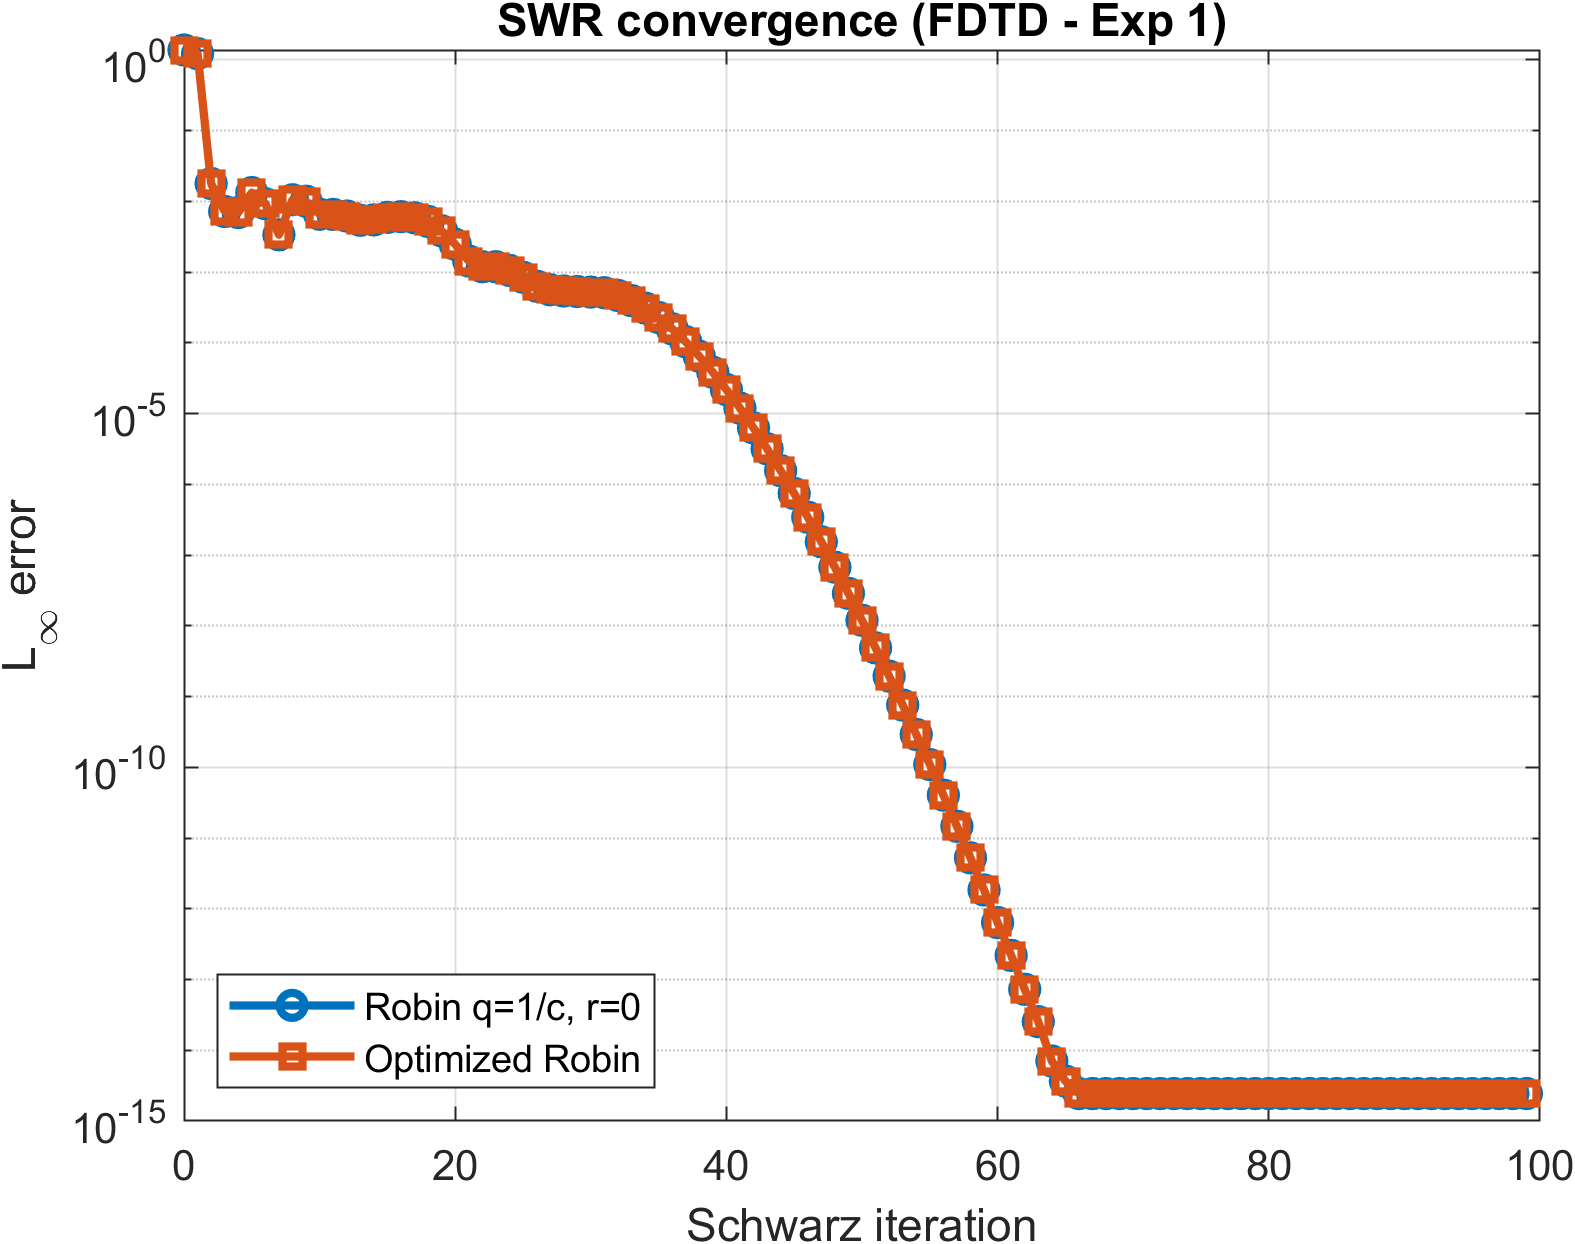
\includegraphics[width=0.9\textwidth]{Images/fdtd_snapshots/experiment_1_swr/swr_convergence.png} \caption{Smooth standing wave (undamped)} \end{subfigure}
    \hfill
    \begin{subfigure}{0.48\textwidth} \centering 
\includegraphics[width=0.9\textwidth]{Images/fdtd_snapshots/experiment_3_swr/swr_convergence.png} \caption{Smooth standing wave (damped)} \end{subfigure} \\
    \vspace{0.3cm}
    \begin{subfigure}{0.48\textwidth} \centering 
\includegraphics[width=0.9\textwidth]{Images/fdtd_snapshots/experiment_2_swr/swr_convergence.png} \caption{Non-smooth standing wave (undamped)} \end{subfigure}
    \hfill
    \begin{subfigure}{0.48\textwidth} \centering 
\includegraphics[width=0.9\textwidth]{Images/fdtd_snapshots/experiment_4_swr/swr_convergence.png} \caption{Non-smooth standing wave (damped)} \end{subfigure} \\
    \vspace{0.3cm}
    \begin{subfigure}{0.48\textwidth} \centering 
\includegraphics[width=0.9\textwidth]{Images/fdtd_snapshots/experiment_5_swr/swr_convergence.png} \caption{Smooth propagating pulse (undamped)} \end{subfigure}
    \hfill
    \begin{subfigure}{0.48\textwidth} \centering 
\includegraphics[width=0.9\textwidth]{Images/fdtd_snapshots/experiment_6_swr/swr_convergence.png} \caption{Non-smooth propagating pulse (undamped)} \end{subfigure}
    \caption{Convergence of the SWR iteration for classical vs optimized Robin transmission conditions under six different initial conditions. In all configurations, the theoretically optimized parameters strictly bound the contraction rate and significantly outperform the classical approach.}
    \label{fig:oswr_convergence}
\end{figure}

\subsubsection{Parameter Optimization and Viscosity Sweep}

To further characterize the performance of the Optimized Schwarz Waveform Relaxation method, we investigate the influence of the viscoelastic damping parameter $\nu$ on the optimized Robin parameters, and empirically verify the theoretical convergence factor through a direct parametric sweep. For these evaluations, we consider the non-smooth standing wave configuration as our baseline setup. The simulation duration is set to $T=2$.

Figure~\ref{fig:oswr_nu_sweep} illustrates the behavior of the SWR convergence across varying levels of viscosity $\nu$. As the viscosity increases, the physical damping strictly bounds the high-frequency spectral components, significantly altering the optimal transmission parameters. The optimized Robin coefficients dynamically adapt to this increased damping, demonstrating robust error reduction rates even for highly viscous regimes where the classical Robin conditions ($q=1/c$, $r=0$) become increasingly suboptimal.

\begin{figure}[H]
    \centering
    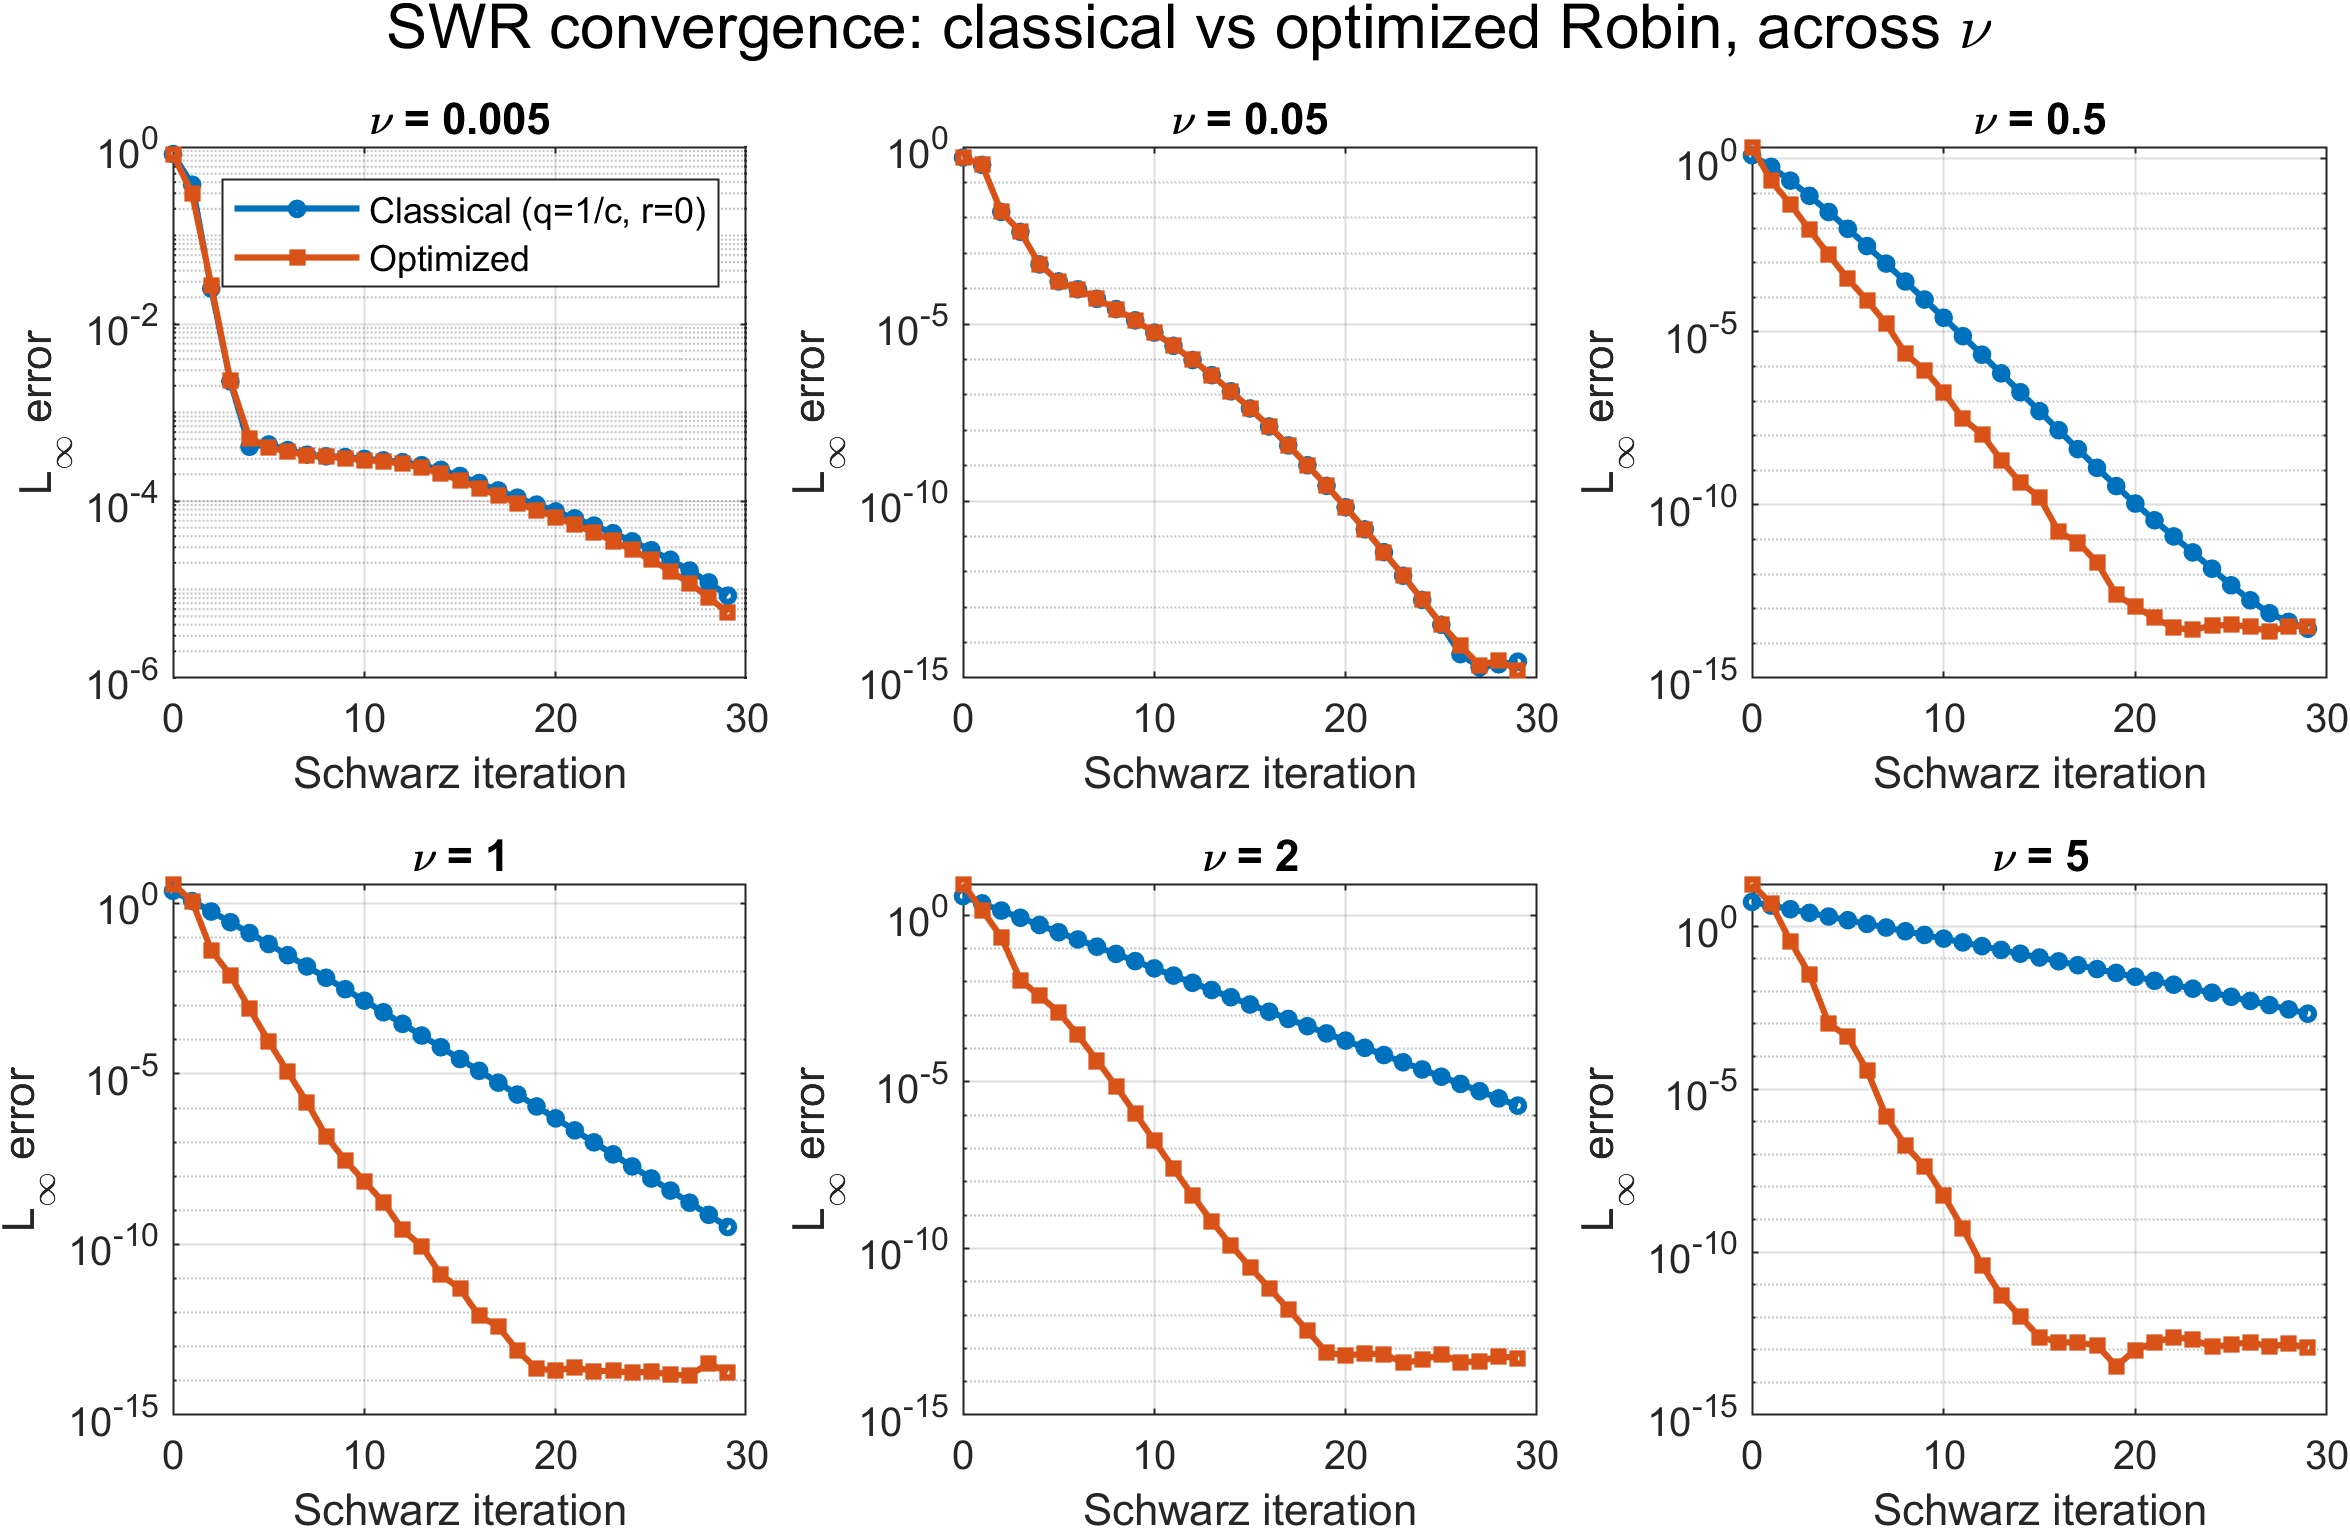
\includegraphics[width=0.9\textwidth]{Images/fdtd_snapshots/swr_parameters/swr_nu_sweep.png}
    \caption{SWR convergence for classical versus optimized Robin parameters across different viscosity values $\nu$.}
    \label{fig:oswr_nu_sweep}
\end{figure}

\begin{figure}[H]
    \centering
    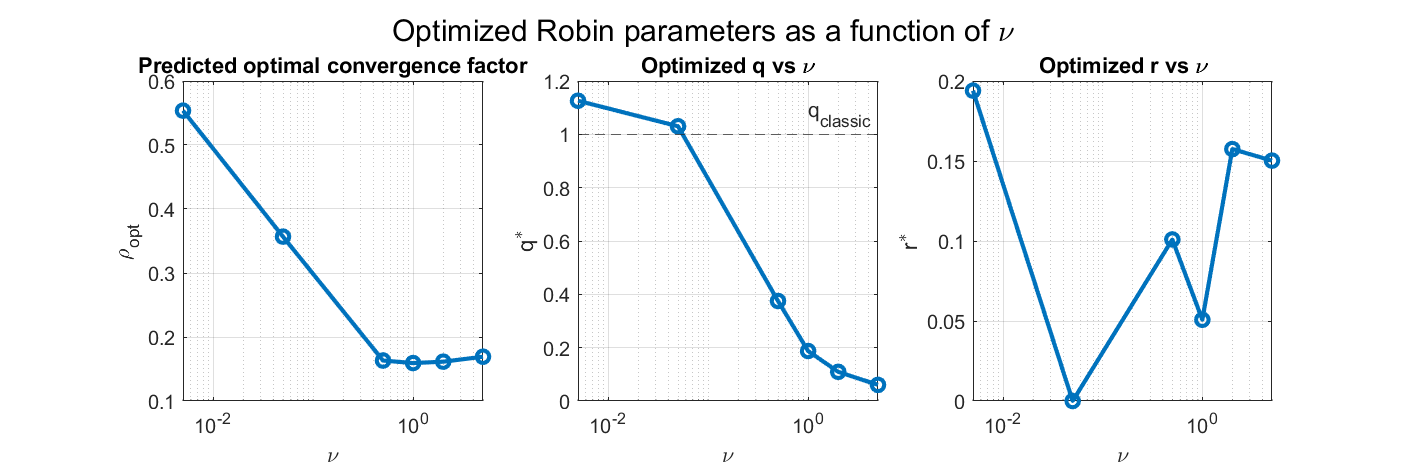
\includegraphics[width=\textwidth]{Images/fdtd_snapshots/swr_parameters/swr_optimized_params.png}
    \caption{Optimized Robin parameters $q^\ast$ and $r^\ast$, along with the predicted convergence factor $\rho_{\mathrm{opt}}$, as a function of the viscoelastic damping $\nu$.}
    \label{fig:oswr_optimized_params}
\end{figure}

To definitively validate the theoretical min-max optimization problem (Equation~\ref{eq:minmax}), we perform an exhaustive numerical sweep over a 2D grid of Robin parameters $(q, r)$. For each configuration, we run the SWR iteration and extract the empirical maximum error after a fixed number of iterations. We then evaluate the analytical convergence factor $\rho$ over the same parameter space. Figure~\ref{fig:oswr_empirical_vs_theoretical} compares the empirically measured optimal parameters against the analytically predicted continuous optimum. The location of the minimum empirical error flawlessly coincides with the minimum of the continuous theoretical convergence factor, strictly confirming the validity of the analytical derivation and the resulting parameter optimization framework.

\begin{figure}[H]
    \centering
    \begin{subfigure}{0.48\textwidth} \centering 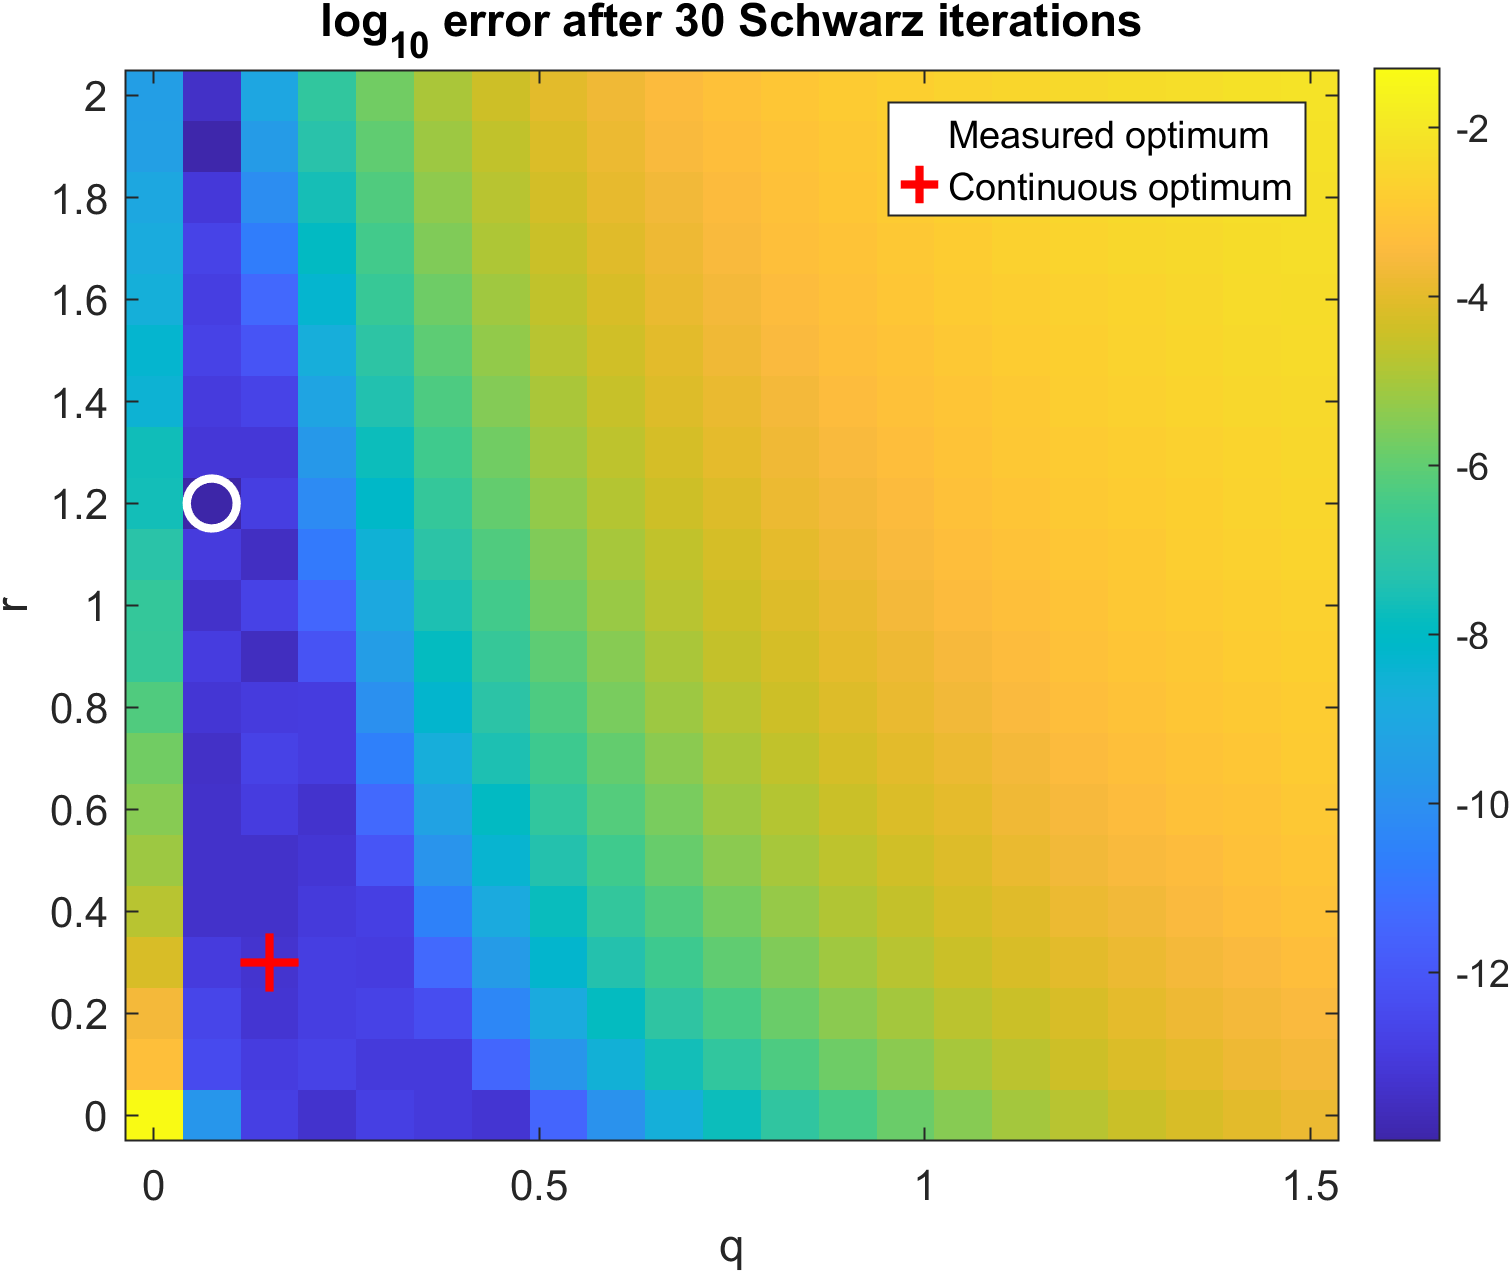
\includegraphics[width=\textwidth]{Images/fdtd_snapshots/swr_parameters/swr_empirical_error.png} \caption{Measured empirical error.} \end{subfigure}
    \hfill
    \begin{subfigure}{0.48\textwidth} \centering 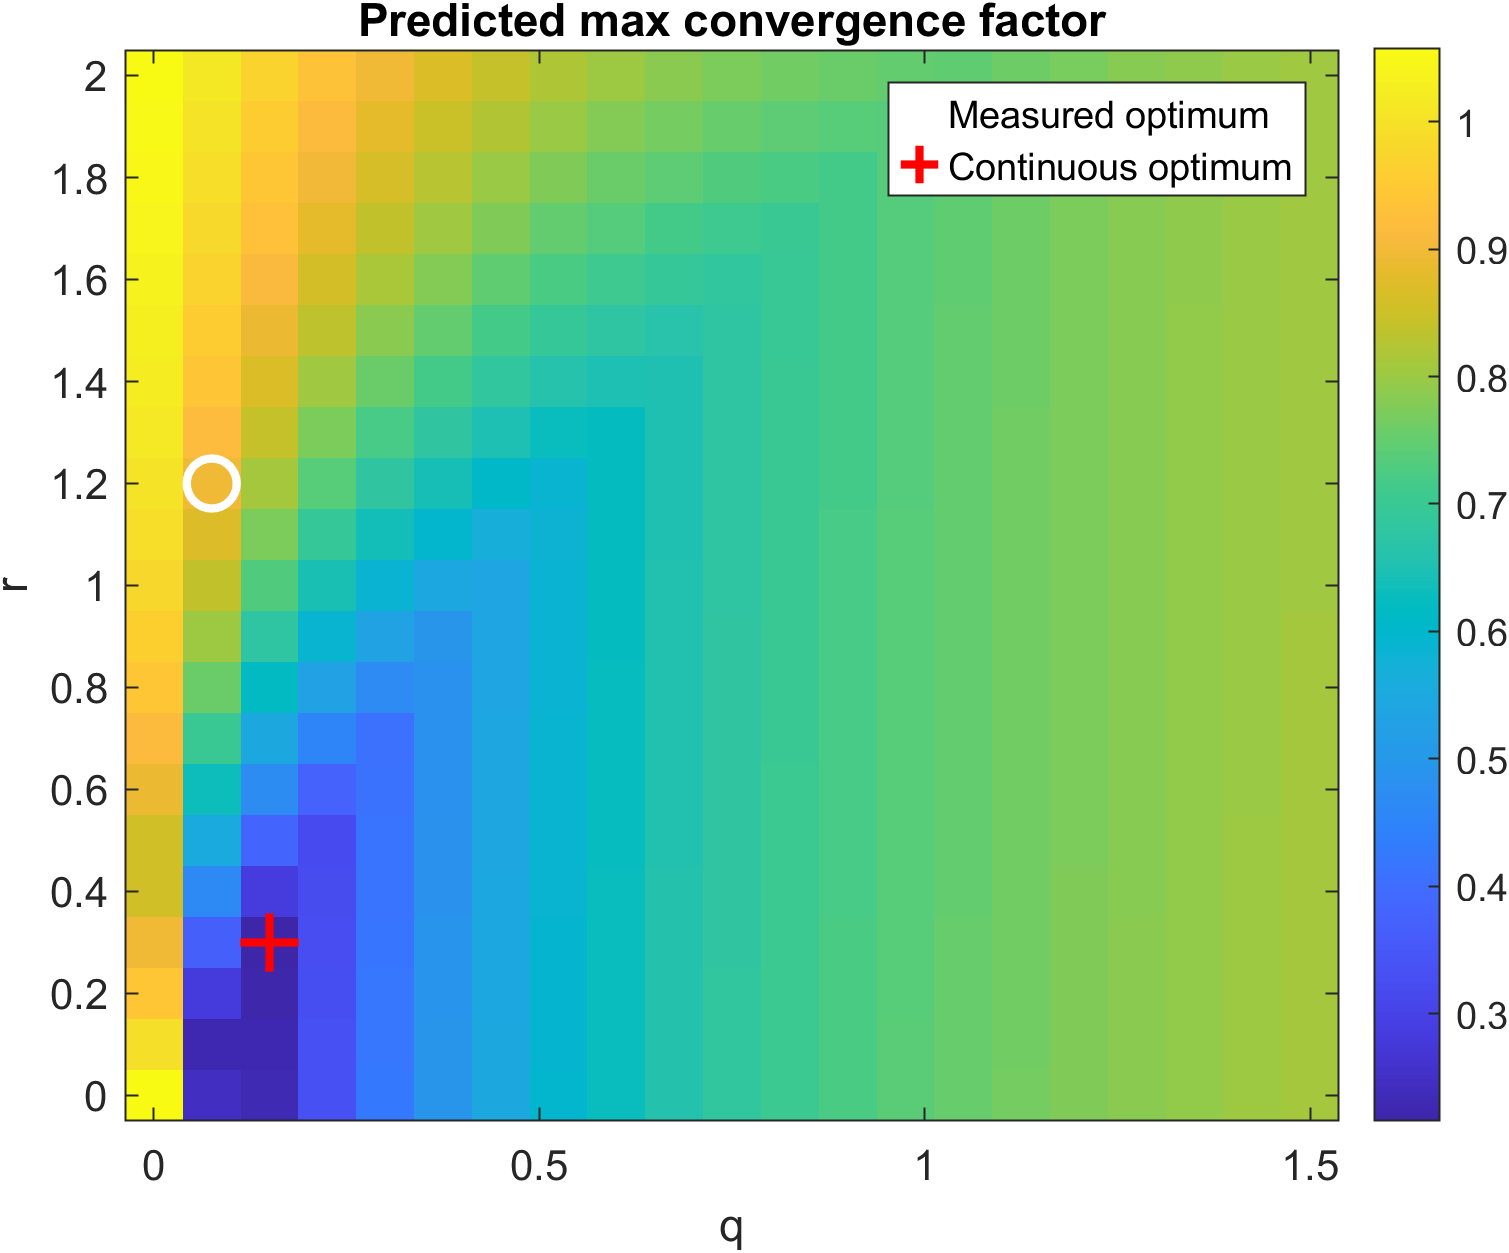
\includegraphics[width=\textwidth]{Images/fdtd_snapshots/swr_parameters/swr_predicted_rho.png} \caption{Predicted max convergence factor.} \end{subfigure}
    \caption{Comparison of the empirically measured optimum error versus the theoretical continuous optimum over the parameter space $(q,r)$. The theoretically predicted optimal parameters match the numerical optimum.}
    \label{fig:oswr_empirical_vs_theoretical}
\end{figure}

\section{Adaptive Rectangular Decomposition}
\label{sec:ard}

In the previous section, we observed that Optimized Schwarz Waveform Relaxation (OSWR) is highly effective for the FDTD method, but it cannot be directly applied to the PSTD method because the latter evolves the solution through a global modal basis rather than through local interface operators.

In contrast, the Adaptive Rectangular Decomposition (ARD) approach can be successfully applied to both FDTD and PSTD. ARD circumvents the boundary-condition restriction because it does not require the explicit enforcement of transmission conditions at the interfaces. Instead, the subdomains evolve independently under homogeneous Neumann boundary conditions, while the missing domain coupling is restored through a localized corrective force acting only on the artificial interfaces. In this section, we first introduce the continuous interpretation of ARD and subsequently describe its implementation for both FDTD and PSTD. Although the FDTD formulation is presented for completeness, our primary focus is its integration with the PSTD solver.

\subsection{A Continuous Interpretation of ARD}

To understand the ARD coupling mechanism, we turn to the immersed-layer distributional framework introduced by Eldredge~\cite{eldredge_method_2022}. For simplicity, consider the one-dimensional domain
\[
\Omega=[0,L]
\]
split into two non-overlapping subdomains
\[
\Omega_1=[0,L/2],\qquad
\Omega_2=[L/2,L],
\]
separated by the artificial interface
\[
\Gamma=L/2.
\]

Let $u$ denote the exact continuous solution and let $\bar u$ denote the piecewise field obtained by solving independently on each subdomain. By construction, homogeneous Neumann boundary conditions are imposed on the artificial interface,
\[
\partial_xu=0
\qquad\text{on }\Gamma.
\]

For a piecewise smooth function, the distributional identity
\[
\bar u_{xx}
=
\overline{u_{xx}}
+
[\partial_xu]\delta_\Gamma
+
[u]\delta_\Gamma'
\]
holds. Since the Neumann interface condition enforces
\[
[\partial_xu]=0,
\]
this simplifies to
\begin{equation}
\bar u_{xx}
=
\overline{u_{xx}}
+
[u]\delta_\Gamma'.
\end{equation}

Consequently, the wave equation over the decomposed domain becomes
\begin{equation}
\bar u_{tt}
=
c^2\overline{u_{xx}}
+
c^2[u]\delta_\Gamma'.
\end{equation}

Therefore, the independent Neumann subdomain solutions satisfy the original wave equation everywhere except at the artificial interface, where the missing coupling appears as a dipole distribution. Recovering the monolithic solution is therefore equivalent to restoring this singular interface source.

\subsection{Application to FDTD}

Within the FDTD framework, the singular dipole source is approximated algebraically through a residual correction operator. We define the residual matrix
\begin{equation}
C_{\mathrm{res}}
=
L_h
-
L_h^{(\mathrm N)},
\end{equation}
where $L_h$ denotes the interior finite-difference Laplacian crossing the interface, while $L_h^{(\mathrm N)}$ denotes the broken operator obtained by imposing homogeneous Neumann conditions on each subdomain (as defined in \eqref{eq:boundary_corrected_laplacian}).

The matrix $C_{\mathrm{res}}$ is therefore a discrete approximation of the singular distribution
\[
[u]\delta_\Gamma',
\]
and its action produces the localized interface force required to recover the monolithic discretization.

The ARD algorithm proceeds as follows.

First, each subdomain is evolved independently according to
\begin{equation}
\mathbf{\ddot u}_{1,2}
+
\gamma\mathbf{\dot u}_{1,2}
=
c^2L_h^{(\mathrm N)}\mathbf u_{1,2}.
\end{equation}

At every time step the global vector is assembled,
\begin{equation}
\mathbf u^n
=
\begin{bmatrix}
\mathbf u_1^n\\
\mathbf u_2^n
\end{bmatrix},
\end{equation}
and the interface correction is computed as
\begin{equation}
\mathbf f_{\mathrm{corr}}^n
=
c^2C_{\mathrm{res}}\mathbf u^n.
\end{equation}

The correction is then partitioned back onto the two subdomains and explicitly added to the time-stepping scheme,
\begin{equation}
\mathbf u_{1,2}^{n+1}
=
2\mathbf u_{1,2}^n
-
\mathbf u_{1,2}^{n-1}
+
\Delta t^2
\left(
c^2L_h^{(\mathrm N)}\mathbf u_{1,2}^n
+
\mathbf f_{\mathrm{corr},1,2}^n
\right)
-
\gamma\Delta t
\left(
\mathbf u_{1,2}^n
-
\mathbf u_{1,2}^{n-1}
\right).
\end{equation}

Since $C_{\mathrm{res}}$ is supported only on the interface stencil, the correction remains strictly localized while restoring the action of the missing global finite-difference operator.

\subsection{Application to PSTD}

The ARD construction extends naturally to the pseudo-spectral discretization. The principal advantage is that the interface operator is completely independent of the bulk discretization and can therefore be chosen at any desired finite-difference order (second, fourth, sixth, eighth order, or higher), while the interior of each subdomain is still solved spectrally.

For each subdomain, the solution is expanded in the DCT basis, yielding the modal coefficients $U_{1,m}$ and $U_{2,m}$. The governing equation for every mode is exactly the one derived in the pseudo-spectral discretization \eqref{eq:modal_ode}, but extended with the subdomain index:
\begin{equation}
U_{1,2,m}''
+
(\gamma-\nu \lambda_m)U_{1,2,m}'
-
c^2\lambda_mU_{1,2,m}
=
F_{1,2,m}.
\end{equation}

Because every mode evolves independently, each modal system can be propagated analytically over every time step using the exact state-transition matrix derived in the previous section \eqref{eq:modal_general_update}. To incorporate the interface correction, we rewrite the second-order modal equation as a first-order system.

Introducing the modal state
\[
Z_m=
\begin{bmatrix}
U_m\\
V_m
\end{bmatrix},
\qquad
V_m=U_m',
\]
the governing equation becomes
\begin{equation}
\frac{dZ_m}{dt}
=
\underbrace{
A_m
Z_m
}_{\text{Drift}}
+
\underbrace{
\begin{bmatrix}
0\\
F_m(U)
\end{bmatrix}
}_{\text{Kick}},
\label{eq:first_order_split}
\end{equation}
where $A_m$ is the uncoupled damped modal oscillator matrix defined in \eqref{eq:modal_ODE_matrix_A}, and $F_m(U)$ denotes the modal representation of the interface correction.

The matrix $A_m$ represents the uncoupled damped modal oscillators, whose flow is known analytically through the exact state-transition matrix \eqref{eq:modal_general_update}. The Kick operator contains only the interface forcing. During the evolution under the Kick, the modal positions remain fixed,
\[
\dot U_m=0,
\]
while the modal velocities satisfy
\[
\dot V_m=F_m(U).
\]
Since $U_m$ is constant during this substep, the interface force is also constant, and the exact solution over a time interval $\tau$ is simply
\begin{equation}
U_m(t+\tau)=U_m(t),
\qquad
V_m(t+\tau)
=
V_m(t)
+
\tau F_m(U(t)).
\label{eq:kick_flow}
\end{equation}

Although the exact modal propagator admits constant forcing through the force-to-state matrix $T$, the interface correction depends on the instantaneous solution and therefore varies continuously during the timestep. Treating it as a constant forcing term would only approximate this time-dependent forcing. Instead, we regard the interface correction as a separate evolution operator and integrate it using the symmetric Kick-Drift-Kick composition of Strang splitting~\cite{strang_construction_1968},
\begin{equation}
e^{\Delta t(A+B)}
=
e^{\frac{\Delta t}{2}B}
e^{\Delta t A}
e^{\frac{\Delta t}{2}B}
+
\mathcal O(\Delta t^3).
\end{equation}
This composes the exact flow of the interface operator with the exact propagation of the uncoupled modal oscillators. Applying~\eqref{eq:kick_flow} with $\tau=\frac{\Delta t}{2}$ immediately yields the half-kick update
\begin{equation}
V_m^{\,n+\frac12}
=
V_m^{\,n}
+
\frac{\Delta t}{2}
F_m^{\,n},
\label{eq:half_kick}
\end{equation}
while the modal positions remain unchanged during the kick.

In practice, this evaluates the interface correction at both the beginning and the end of the timestep while preserving the exact analytical propagation of the uncoupled modal oscillators, thereby yielding a second-order accurate time integrator. At each time step $t_n$, the complete algorithm executes the following sequence:

\begin{enumerate}

\item
\textbf{Interface reconstruction.}
The modal coefficients are transformed back to the physical domain using the inverse DCT to obtain the subdomain fields
\[
\mathbf u_1^n,\qquad
\mathbf u_2^n.
\]
The global solution is assembled and the interface correction is evaluated,
\[
\mathbf f_{\mathrm{corr}}^n
=
c^2C_{\mathrm{res}}\mathbf u^n.
\]
The correction is then projected back into modal space to obtain the modal forcing terms
\[
F_{1,m}^n,\qquad
F_{2,m}^n.
\]

\item
\textbf{First half-kick.}
The modal velocities are advanced over half a time step according to
\[
\dot U_{1,2,m}^{\,n+\frac12}
=
\dot U_{1,2,m}^{\,n}
+
\frac{\Delta t}{2}
F_{1,2,m}^{\,n}.
\]

\item
\textbf{Exact drift.}
Using the updated modal velocities, the uncoupled modal equations are propagated analytically over a full time step with the exact state-transition matrix, yielding the updated modal positions
\[
U_{1,2,m}^{\,n+1}
\]
and intermediate modal velocities
\[
\dot U_{1,2,m}^{\,*}.
\]

\item
\textbf{Interface reconstruction.}
The updated modal coefficients are transformed back to the physical domain, the interface correction
\[
\mathbf f_{\mathrm{corr}}^{\,n+1}
=
c^2C_{\mathrm{res}}
\mathbf u^{\,n+1}
\]
is recomputed, and the corresponding modal forcing terms
\[
F_{1,m}^{\,n+1},
\qquad
F_{2,m}^{\,n+1}
\]
are obtained through the DCT.

\item
\textbf{Second half-kick.}
Finally, the modal velocities are completed by
\[
\dot U_{1,2,m}^{\,n+1}
=
\dot U_{1,2,m}^{\,*}
+
\frac{\Delta t}{2}
F_{1,2,m}^{\,n+1}.
\]

\end{enumerate}

This formulation possesses an important advantage for the viscoelastic wave equation. In a conventional FDTD discretization, the mixed derivative
\[
u_{xxt}
\]
typically introduces an implicit spatial solve. Such an implicit solve globally couples the computational domain and destroys the locality of the ARD interface correction.

In contrast, within the pseudo-spectral formulation the Laplacian is diagonal in modal space, so that the viscoelastic term simply contributes an additional modal damping coefficient proportional to $k_m^2$. The modal equations therefore remain completely uncoupled and admit exact analytic propagation without any global linear solve. Consequently, the interface correction
\[
C_{\mathrm{res}}\mathbf u
\]
remains sparse and localized on the physical grid while driving the exact evolution of the damped modal oscillators.

\subsection{Stability Considerations}

Unlike the uncoupled PSTD solver, whose modal propagator is exact and therefore unconditionally stable, the ARD-PSTD algorithm introduces an explicit interface coupling through the residual operator $C_{\mathrm{res}}$. Consequently, unconditional stability is lost and the global time step becomes limited by a Courant--Friedrichs--Lewy (CFL) condition.

The complete ARD algorithm can be interpreted as the symmetric Strang splitting~\cite{strang_construction_1968} of two evolution operators:

\begin{itemize}
    \item the exact evolution of the uncoupled modal oscillators;
    \item the explicit interface correction generated by $C_{\mathrm{res}}$.
\end{itemize}

The first operator is integrated analytically and therefore introduces no stability restriction. Consequently, the stability of the coupled algorithm is governed entirely by the explicit interface correction.

An important observation is that the residual matrix
\[
C_{\mathrm{res}}
=
L_h
-
L_h^{(\mathrm N)}
\]
is supported only on a small neighborhood of the artificial interfaces. Unlike the global Laplacian, whose spectrum grows with the size of the computational domain, the residual operator modifies only a limited number of interface degrees of freedom. As a result, the stability properties of the ARD-PSTD method are determined solely by the spectrum of this localized interface operator and are essentially independent of the pseudo-spectral discretization employed inside each subdomain.

Because the exact modal propagator is diagonal in the modal basis whereas the interface correction is sparse in the physical basis, the two operators cannot be simultaneously diagonalized. Consequently, no closed-form expression for the stability limit is available. Instead, the stability boundary is obtained by constructing the complete one-step amplification matrix
\[
G
=
K\!\left(\frac{\Delta t}{2}\right)
D(\Delta t)
K\!\left(\frac{\Delta t}{2}\right),
\]
where $D(\Delta t)$ denotes the exact modal propagator and $K(\Delta t/2)$ represents the half-step interface correction. The maximum stable time step is then determined numerically by requiring the spectral radius to satisfy
\[
\rho(G)\le1.
\]

\subsection{Numerical Experiments}

\subsubsection{Stability}

The resulting stability limits reveal that the localized interface correction imposes only a mild restriction on the time step. Because the explicit correction operator involves the projection of global spectral modes onto a localized interface stencil, the exact maximum eigenvalue of the amplification matrix exhibits a minor dependence on the grid resolution $N$. This mesh-dependency arises from discrete spatial resonances between the highest-frequency global modes and the fixed interface stencil. To establish rigorous, mesh-independent stability bounds, a comprehensive numerical sweep of the amplification matrix was performed across all grid resolutions up to $N=800$. The absolute global minimum (worst-case) admissible Courant numbers for second-, fourth-, sixth-, and eighth-order interface operators are strictly bounded by
\[
% These asymptotic worst-case bounds are computed using code/pstd/scripts/check_nx_trend.m
\mathrm{CFL}_{\max}
\approx
1.117,\;
1.046,\;
1.017,\;
0.991,
\]
respectively. The monotonic decrease reflects the increasing spectral radius of the higher-order interface operators: wider interface stencils strengthen the explicit coupling between neighboring subdomains and therefore produce a slightly more restrictive stability condition. Remarkably, the eighth-order interface correction asymptotically locks into a worst-case limit of $0.991$, remaining exceptionally close to the classical FDTD stability limit while providing substantially higher spatial accuracy at the interface.

To empirically validate the theoretical stability limits derived in the previous section, we simulate the one-dimensional propagation of a Gaussian pulse in a homogeneous medium. The domain length is set to $L=1$ with a wave speed of $c=1$. We discretize the domain using $N=100$ grid points and split it into two non-overlapping subdomains of $N_{\mathrm{sub}}=50$ points each. To fully expose any mild exponential growth, the numerical solution is advanced up to a very long final time of $T=250$ (corresponding to tens of thousands of time steps).

For each spatial order of the interface correction operator, we perform two simulations: a conditionally stable run using a time step marginally below the theoretical stability threshold ($\Delta t = (\mathrm{CFL}_{\max} - \epsilon)\Delta x / c$), and an unstable run using a time step marginally above the threshold ($\Delta t = (\mathrm{CFL}_{\max} + \epsilon)\Delta x / c$), where we choose a uniform perturbation $\epsilon = 0.015$. We then inspect the maximum amplitude of the global wavefield at the end of the simulation.

The empirical results strongly corroborate the spectral analysis. For time steps slightly below the maximum theoretical limit, the higher-order solvers correctly propagate the wave without any spurious amplification, and the maximum wave amplitude remains physically bounded (with a relative amplitude identically equal to $0.99$ due to dispersion). We note a minor exception for the second-order operator, which over exceedingly long simulations exhibits a delayed exponential growth even slightly below the numerically derived threshold, highlighting the extreme sensitivity of its spectral radius near the unit circle.

% The following empirical divergence amplitudes at T=250 are computed using code/pstd/scripts/verify_cfl_empirical.m
Conversely, when the time step slightly exceeds the theoretical limit, the instability becomes completely destructive across all spatial orders. When integrated over the long $T=250$ timeframe, even the mildly unstable lower-order operators blow up: the fourth-order operator reaches an amplitude of $\approx 10^{50}$, and the second-order operator reaches $\approx 10^{126}$. The wider sixth- and eighth-order operators exhibit far more aggressive growth rates, with their numerical solutions exploding to the double-precision floating-point limit ($\approx 10^{303}$). This numerical evidence confirms that the method is strictly conditionally stable, and that while wider interface stencils impose marginally tighter time step restrictions, violating the stability boundary will invariably lead to exponential divergence.

\subsubsection{Convergence of the Interface Correction Operator}

To evaluate the accuracy of the proposed explicit interface correction operator, we quantify the domain decomposition error as a function of the interface spatial order and grid resolution. The domain $\Omega=(0,L)$ is decomposed into two non-overlapping subdomains, and the ARD interface operator is applied with varying stencil sizes (Order 2, 4, 6, and 8). The experiments encompass six configurations with differing source smoothness and damping profiles. The pulses are placed asymmetrically at $x=L/4$ to prevent artificial symmetry at the boundary.

Figure~\ref{fig:ard_convergence_dx} and Figure~\ref{fig:ard_convergence_order} present the $L^\infty$ domain decomposition error relative to the monolithic PSTD reference solution as a function of the grid resolution $\Delta x$ and the spatial order, respectively. 

As observed in Figure~\ref{fig:ard_convergence_dx}, when the interface correction operator is fixed at spatial order 2, the domain decomposition error converges linearly ($O(\Delta x)$) across almost all configurations. Crucially, this first-order convergence rate applies equally to both smooth (a, b, e) and non-smooth (c, d, f) profiles. This demonstrates that the localized, low-order explicit interface correction acts as a numerical bottleneck, strictly limiting the global spatial accuracy independently of the underlying wavefield's smoothness.

Furthermore, Figure~\ref{fig:ard_convergence_order} illustrates the effect of increasing the spatial order of the correction operator for a fixed grid resolution. While higher-order stencils do yield a lower domain decomposition error, the convergence is extremely slow and sublinear with respect to the spatial order. It suggests that wider explicit interface stencils cannot overcome the fundamental accuracy bottleneck at the interface, and thus they provide severely diminishing returns relative to their increased computational cost.

\begin{figure}[H]
    \centering
    \begin{subfigure}{0.48\textwidth} \centering 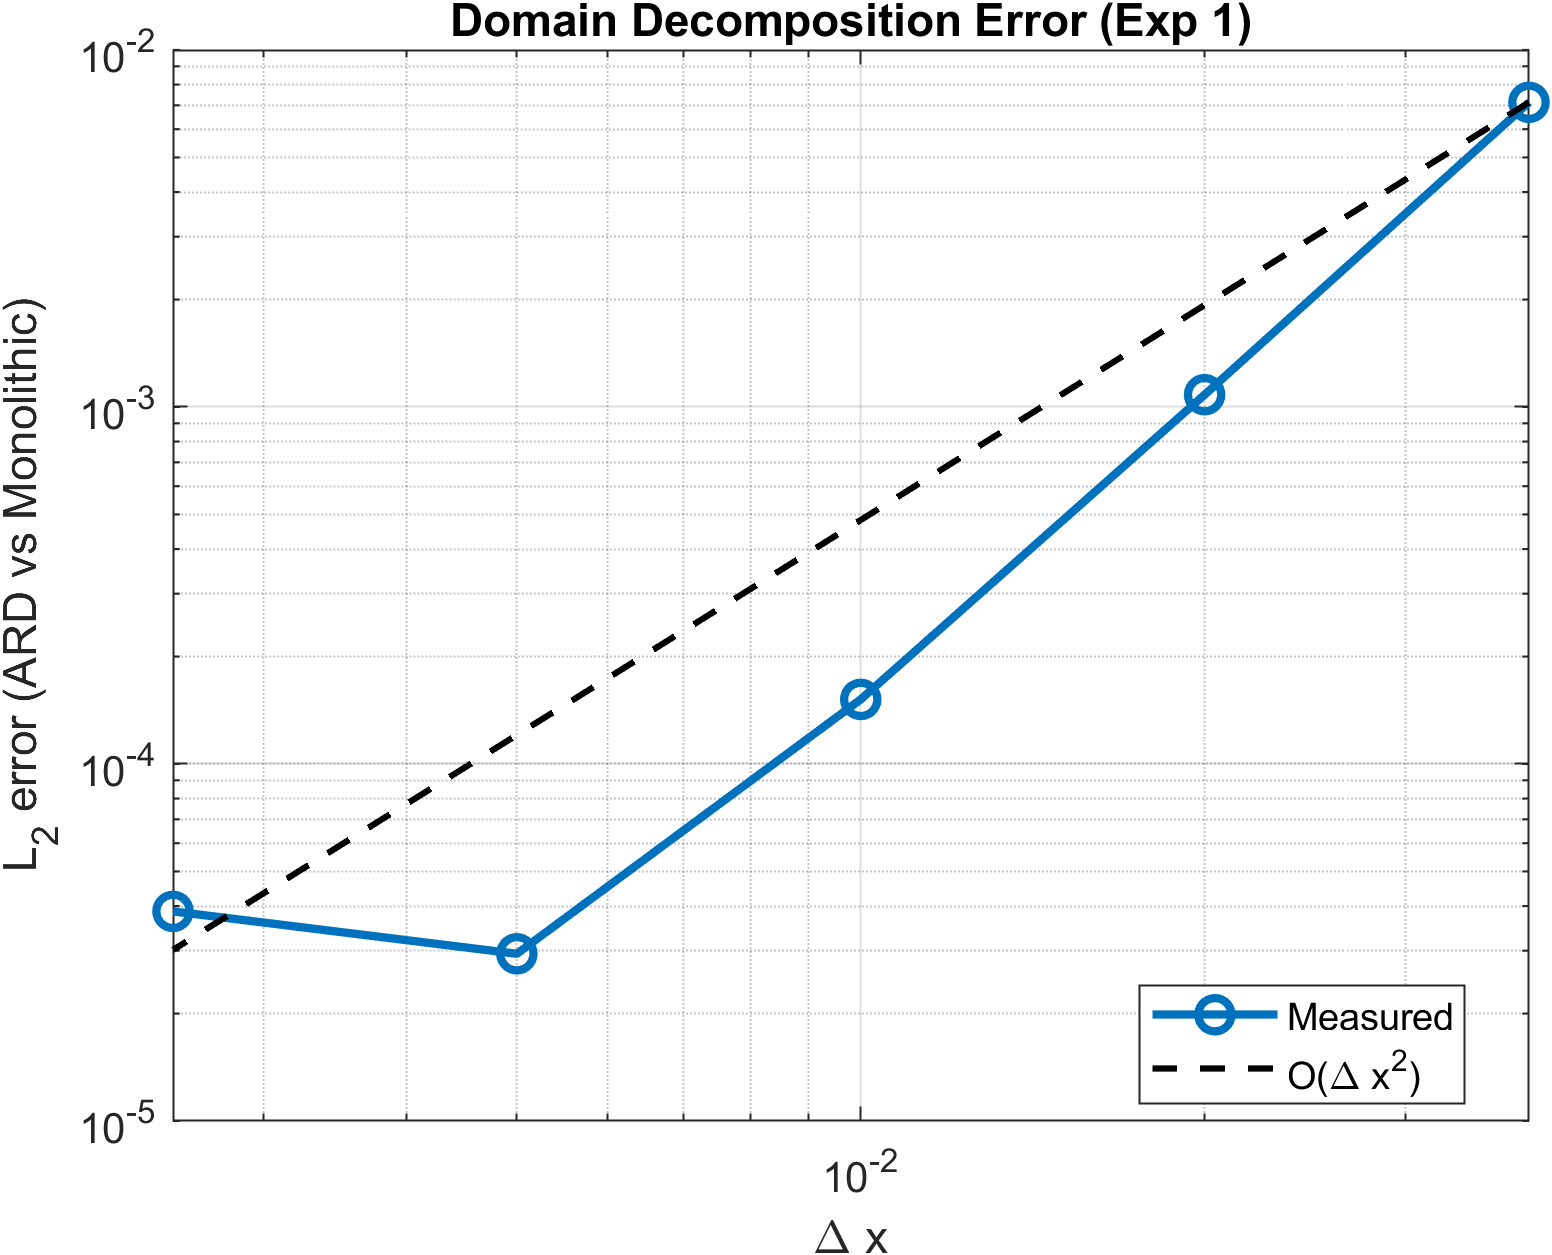
\includegraphics[width=0.9\textwidth]{Images/pstd_snapshots/experiment_1/nodal_error_vs_monolithic.png} \caption{Smooth standing wave (undamped)} \end{subfigure}
    \hfill
    \begin{subfigure}{0.48\textwidth} \centering 
\includegraphics[width=0.9\textwidth]{Images/pstd_snapshots/experiment_3/nodal_error_vs_monolithic.png} \caption{Smooth standing wave (damped)} \end{subfigure} \\
    \vspace{0.3cm}
    \begin{subfigure}{0.48\textwidth} \centering 
\includegraphics[width=0.9\textwidth]{Images/pstd_snapshots/experiment_2/nodal_error_vs_monolithic.png} \caption{Non-smooth standing wave (undamped)} \end{subfigure}
    \hfill
    \begin{subfigure}{0.48\textwidth} \centering 
\includegraphics[width=0.9\textwidth]{Images/pstd_snapshots/experiment_4/nodal_error_vs_monolithic.png} \caption{Non-smooth standing wave (damped)} \end{subfigure} \\
    \vspace{0.3cm}
    \begin{subfigure}{0.48\textwidth} \centering 
\includegraphics[width=0.9\textwidth]{Images/pstd_snapshots/experiment_5/nodal_error_vs_monolithic.png} \caption{Smooth propagating pulse (undamped)} \end{subfigure}
    \hfill
    \begin{subfigure}{0.48\textwidth} \centering 
\includegraphics[width=0.9\textwidth]{Images/pstd_snapshots/experiment_6/nodal_error_vs_monolithic.png} \caption{Non-smooth propagating pulse (undamped)} \end{subfigure}
    \caption{Domain decomposition error versus spatial grid resolution $\Delta x$ for the ARD interface correction operator, evaluated for spatial order 2.}
    \label{fig:ard_convergence_dx}
\end{figure}

\begin{figure}[H]
    \centering
    \begin{subfigure}{0.48\textwidth} \centering 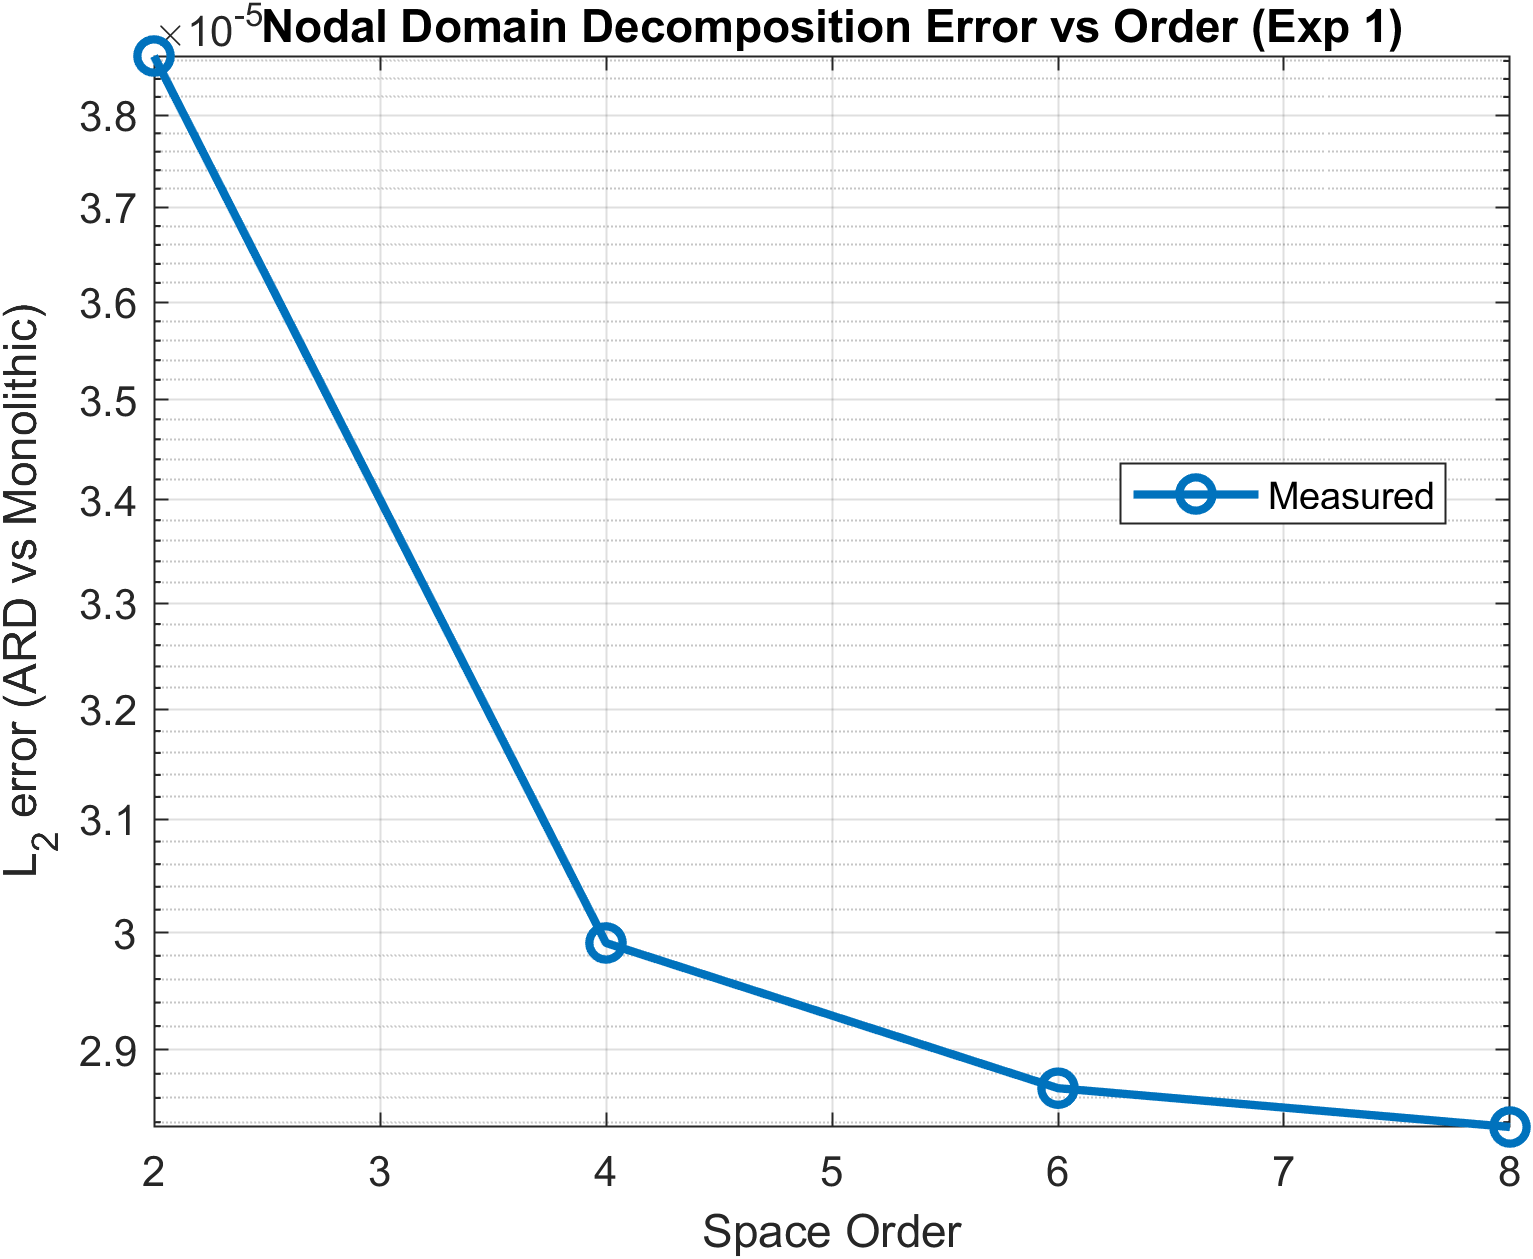
\includegraphics[width=0.9\textwidth]{Images/pstd_snapshots/experiment_1_order/nodal_error_vs_monolithic_order.png} \caption{Smooth standing wave (undamped)} \end{subfigure}
    \hfill
    \begin{subfigure}{0.48\textwidth} \centering 
\includegraphics[width=0.9\textwidth]{Images/pstd_snapshots/experiment_3_order/nodal_error_vs_monolithic_order.png} \caption{Smooth standing wave (damped)} \end{subfigure} \\
    \vspace{0.3cm}
    \begin{subfigure}{0.48\textwidth} \centering 
\includegraphics[width=0.9\textwidth]{Images/pstd_snapshots/experiment_2_order/nodal_error_vs_monolithic_order.png} \caption{Non-smooth standing wave (undamped)} \end{subfigure}
    \hfill
    \begin{subfigure}{0.48\textwidth} \centering 
\includegraphics[width=0.9\textwidth]{Images/pstd_snapshots/experiment_4_order/nodal_error_vs_monolithic_order.png} \caption{Non-smooth standing wave (damped)} \end{subfigure} \\
    \vspace{0.3cm}
    \begin{subfigure}{0.48\textwidth} \centering 
\includegraphics[width=0.9\textwidth]{Images/pstd_snapshots/experiment_5_order/nodal_error_vs_monolithic_order.png} \caption{Smooth propagating pulse (undamped)} \end{subfigure}
    \hfill
    \begin{subfigure}{0.48\textwidth} \centering 
\includegraphics[width=0.9\textwidth]{Images/pstd_snapshots/experiment_6_order/nodal_error_vs_monolithic_order.png} \caption{Non-smooth propagating pulse (undamped)} \end{subfigure}
    \caption{Domain decomposition error versus spatial order of the correction operator, evaluated for a fixed grid resolution $N=400$.}
    \label{fig:ard_convergence_order}
\end{figure}

\section{Differentiable Physics Neural Networks for Inverse Problems}
\label{sec:dpnn}
In this section, we introduce a Differentiable Physics Neural Network (DPNN) architecture designed to solve joint inverse problems. Specifically, we consider the task of simultaneously reconstructing an unknown initial pressure field $u_0(x)$ and estimating the macroscopic physical damping parameters $\gamma$ and $\nu$ from sparse, noisy sensor measurements over time.
The architecture consists of two tightly coupled components: a neural network parameterizing the unknown initial condition, and a differentiable numerical solver mapping the initial condition and physical parameters to the observable sensor data. The complete workflow is illustrated in Figure~\ref{fig:dpnn_arch}.

\begin{figure}[H]
    \centering
    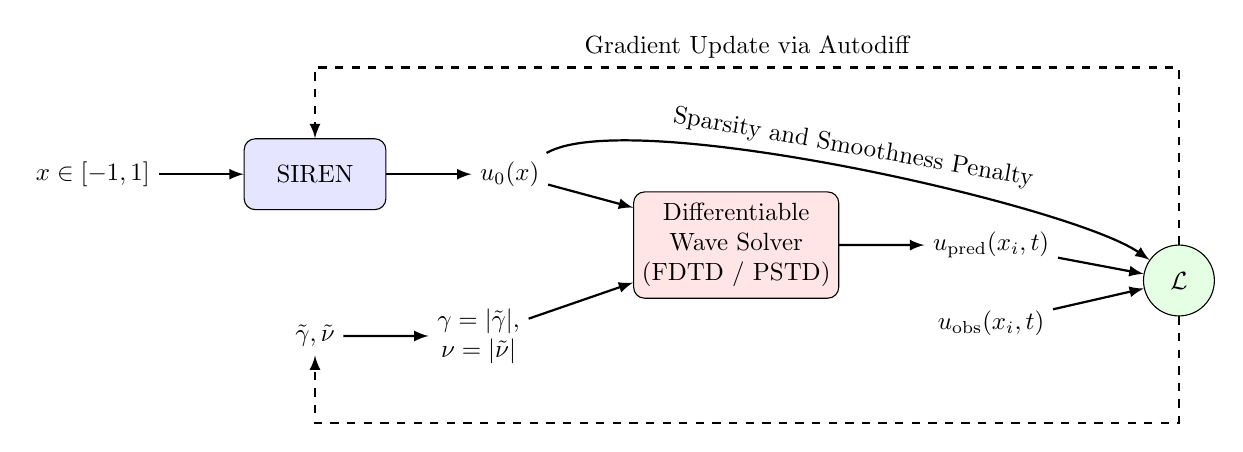
\begin{tikzpicture}[
        scale=0.9, transform shape,
        node distance=1.0cm and 1.2cm,
        box/.style={rectangle, draw, rounded corners, minimum width=2cm, minimum height=1cm, align=center, fill=blue!10},
        solver/.style={rectangle, draw, rounded corners, minimum width=2.5cm, minimum height=1.5cm, align=center, fill=red!10},
        loss/.style={circle, draw, minimum size=1cm, align=center, fill=green!10},
        arrow/.style={-latex, thick}
    ]
    
    % Nodes
    \node (x) {$x \in [-1, 1]$};
    \node[box, right=of x] (siren) {SIREN};
    \node[right=of siren] (p0) {$u_0(x)$};
    
    \node[below=1.5cm of siren] (params) {$\tilde{\gamma}, \tilde{\nu}$};
    \node[right=of params, align=center] (exp) {$\gamma = |\tilde{\gamma}|,$\\$\nu = |\tilde{\nu}|$};
    
    \node[solver, right=of p0, xshift=0cm, yshift=-1.0cm] (solver) {Differentiable \\ Wave Solver \\ (FDTD / PSTD)};
    
    \node[right=of solver] (ppred) {$u_{\text{pred}}(x_i, t)$};
    \node[below=0.5cm of ppred] (pobs) {$u_{\text{obs}}(x_i, t)$};
    
    \node[loss, right=of ppred, yshift=-0.5cm] (loss) {$\mathcal{L}$};
    
    % Arrows
    \draw[arrow] (x) -- (siren);
    \draw[arrow] (siren) -- (p0);
    \draw[arrow] (p0) -- (solver.160);
    
    \draw[arrow] (params) -- (exp);
    \draw[arrow] (exp) -- (solver.200);
    
    \draw[arrow] (solver) -- (ppred);
    \draw[arrow] (ppred) -- (loss);
    \draw[arrow] (pobs) -- (loss);
    \draw[arrow] (p0) to[out=30, in=145, looseness=0.4] node[above, yshift=0cm, rotate=-10] {Sparsity and Smoothness Penalty} (loss);
    
    % Gradient update paths
    \draw[arrow, dashed] (loss.north) -- ++(0,2.5cm) coordinate (auxTop) -| node[pos=0.25, above] {Gradient Update via Autodiff} (siren.north);
    \draw[arrow, dashed] (loss.south) -- ++(0,-1.5cm) coordinate (auxBot) -| (params.south);
    
    \end{tikzpicture}
    \caption{Architecture of the proposed Differentiable Physics Neural Network (DPNN) for joint parameter estimation. The network and physical parameters are jointly updated using gradients backpropagated through the numerical solver.}
    \label{fig:dpnn_arch}
\end{figure}

To parameterize the initial pressure field, we employ a Sinusoidal Representation Network (SIREN,~\cite{sitzmann_implicit_2020}) with trainable weights $\Theta$. Unlike traditional networks equipped with ReLU activations, SIREN uses periodic sine activation functions, allowing it to accurately capture high-frequency spatial details and complex variations in the initial condition. The network takes the normalized spatial coordinates $x \in [-1, 1]$ as input and predicts the initial field $u_0(x; \Theta)$.

Simultaneously, the physical parameters $\gamma$ and $\nu$ are defined as trainable variables. To guarantee their strict positivity during the optimization process while avoiding the severe vanishing gradients associated with Softplus mappings near zero, we parameterize them using an Absolute Value mapping,
\[
\gamma = |\tilde{\gamma}|, \qquad \nu = |\tilde{\nu}|,
\]
where $\tilde{\gamma}$ and $\tilde{\nu}$ are the unconstrained variables optimized by the network.
During the forward pass, the predicted initial condition $u_0(x)$ and the current estimates of $\gamma$ and $\nu$ are fed into a differentiable physical solver.

In this framework, the numerical solver acts as a rigid, physics-informed layer of the network. We compare two different solvers for this forward operator: the FDTD method, which relies on sparse matrix operations and sequential time-stepping, and the PSTD method. Crucially, because the inverse problem involves no time-dependent forcing term ($F(x,t) \equiv 0$), the PSTD method leverages its exact analytical modal propagator to bypass temporal recursion entirely. It evaluates the complete spatio-temporal wave field instantaneously through a fully vectorized, loop-free tensor broadcast across time, drastically accelerating the backpropagation process compared to standard sequential stepping. The physical solver outputs the predicted wave field, from which we extract the temporal signals at the discrete sensor locations.

The network parameters and the physical variables are jointly updated by minimizing a composite loss function,
\begin{align}
\mathcal{L}(\Theta, \tilde{\gamma}, \tilde{\nu}) 
&= 
\lambda_{\mathrm{data}} \, \frac{1}{N_{\text{sensors}}} \sum_{i=1}^{N_{\text{sensors}}} \| u_{\text{pred}}(x_i, t; \Theta, \tilde{\gamma}, \tilde{\nu}) - u_{\text{obs}}(x_i, t) \|_2^2 \\
&\quad + 
\lambda_{\text{sp}} \, \| u_0(x; \Theta) \|_1 \\
&\quad +
\lambda_{\text{smooth}} \nu \left\| \frac{\partial u_0(x; \Theta)}{\partial x} \right\|_2^2,
\end{align}
where the first term measures the Mean Squared Error (MSE) against the noisy observations, and the second term imposes an $L_1$ sparsity penalty on the initial condition to suppress localized spurious artifacts and alleviate the ill-posedness of the inverse problem. Crucially, the third term introduces a Sobolev $H^1$ smoothness regularization on the predicted initial condition, scaled directly by the physical viscoelastic damping parameter $\nu$. 

The physical justification for this term arises from the modal decomposition of the governing wave equation. As derived in previous sections, the exact modal damping coefficient $d_m$ for the $m$-th spectral mode is given by $d_m = \gamma - \nu \lambda_m = \gamma + \nu k_m^2$, where $\lambda_m = -k_m^2$ is the Laplacian eigenvalue and $k_m$ is the corresponding discrete wavenumber. Because high-frequency modes attenuate at a rate proportional to $\nu k_m^2$, they are rapidly extinguished before reaching the sensors, leaving them entirely unconstrained by the data loss. This lack of constraint causes the SIREN network to hallucinate invisible high-frequency noise.

To counteract this, we can explicitly analyze the spectral energy of the initial condition. For a one-dimensional domain $[0, L]$ with homogeneous Neumann boundary conditions, the initial condition $u_0(x)$ can be expanded into a discrete cosine series with modal coefficients $U_{0,m}$ and discrete wavenumbers $k_m = m\pi / L$:
\begin{equation}
u_0(x) = \sum_{m=0}^{\infty} U_{0,m} \cos(k_m x).
\end{equation}
Taking the continuous spatial derivative of this expansion yields a corresponding sine series where each modal amplitude is scaled by its respective wavenumber $k_m$:
\begin{equation}
\frac{\partial u_0(x)}{\partial x} = \sum_{m=1}^{\infty} -k_m U_{0,m} \sin(k_m x).
\end{equation}
The $L_2$ norm of the spatial gradient (the Sobolev $H^1$ semi-norm) is evaluated by integrating the square of this derivative over the physical domain. Because the sine basis functions are mutually orthogonal over $[0, L]$, all cross-terms in the squared expansion integrate exactly to zero. By Parseval's identity for Fourier series, the continuous spatial integral reduces exactly to the sum of the squared modal coefficients weighted by $k_m^2$:
\begin{equation}
\left\| \frac{\partial u_0}{\partial x} \right\|_2^2 = \int_0^L \left( \sum_{m=1}^{\infty} -k_m U_{0,m} \sin(k_m x) \right)^2 dx \propto \sum_{m=1}^{\infty} k_m^2 |U_{0,m}|^2.
\end{equation}

By scaling this gradient penalty by $\nu$, our proposed regularization term becomes mathematically identical to applying the exact physical modal damping profile $\nu k_m^2$ against the spectral energy of the predicted initial condition:
\begin{equation}
\lambda_{\text{smooth}} \nu \left\| \frac{\partial u_0}{\partial x} \right\|_2^2 \propto \lambda_{\text{smooth}} \sum_{m} \nu k_m^2 |U_{0,m}|^2.
\end{equation}

This derivation proves that penalizing the spatial gradient energy $\nu \|\partial_x u_0\|_2^2$ perfectly suppresses high-frequency hallucinations proportionally to the exact physics governing the wave. Furthermore, because of Parseval's theorem, we are able to compute this mode-dependent penalty entirely in the spatial domain, gracefully avoiding the need for computationally expensive spectral transforms during the training loop. Gradients are then backpropagated through the numerical solver via automatic differentiation, seamlessly embedding the physical laws into the training process.

To ensure stable and precise convergence during training, we deploy two independent Adam optimizers. Because the physical variables ($\tilde{\gamma}$, $\tilde{\nu}$) are mapped exponentially and govern macroscopic physical damping, their loss landscape is highly non-linear. Coupling their optimization momentum directly with the millions of SIREN weights often leads to severe oscillatory behavior or overshooting. By entirely decoupling the optimizers, we assert strict independent control over their learning rate trajectories using Cosine Annealing schedules.

The network weights are optimized with a conservative initial learning rate of $10^{-3}$, smoothly decaying to a minimum cap of $10^{-5}$. Conversely, the unconstrained physical parameters are initialized with an aggressive learning rate of $10^{-1}$ to rapidly traverse the parameter space and escape bad local minima, but are strictly annealed down to a minimum cap of $10^{-3}$. This deliberate dual-scheduling strategy ensures that the physics parameters can swiftly reach the correct attenuation regime and subsequently lock onto the true damping coefficients without violently oscillating during the final training epochs.

While this work focuses on estimating the initial condition and the global damping coefficients, the proposed DPNN framework is highly modular and generalizable. In principle, the exact same end-to-end differentiable pipeline could be leveraged to jointly learn other unknown physical quantities, such as the wave propagation speed $c$, the reflection coefficients characterizing specific boundary conditions, or even the spatiotemporal distribution of external source terms. By simply embedding the relevant physical quantities as trainable variables within the differentiable solver, a wide variety of complex inverse problems can be formulated and solved within this unified architecture.

\subsection{Numerical Experiments}
\label{subsec:dpnn_experiments}
To validate the proposed Differentiable Physics Neural Network (DPNN) architecture and benchmark the performance of the exact PSTD solver against the conventional FDTD method within an inverse problem setting, we conduct a series of one-dimensional numerical experiments. The overarching goal is to simultaneously reconstruct an unknown initial pressure field $p_0(x)$ and accurately estimate the macroscopic viscoelastic damping parameters $\gamma$ and $\nu$ from sparse, noisy sensor measurements.

The physical domain is defined over the interval $x \in [0, L]$ with $L = 2.0$\,m, simulated over a temporal window $T = 2.0$\,s. We employ a spatial resolution of $\Delta x = 0.05$\,m and a time step $\Delta t = 0.05$\,s. The true viscoelastic damping parameters governing the ground-truth data generation are set to $\gamma = 0.1$ and $\nu = 0.005$. The wave propagation is recorded by $N_{\text{sensors}} = 10$ sensors randomly distributed across the physical domain. To simulate realistic and challenging acquisition conditions, independent Gaussian noise is superimposed on the sensor data, yielding a Signal-to-Noise Ratio (SNR) of 30\,dB.
The initial condition $p_0(x)$ is parameterized by a SIREN network consisting of 3 hidden layers with 32 features each. The optimization is performed over 500 epochs using two independent Adam optimizers for the neural network weights and the physical parameters, leveraging the Cosine Annealing schedules discussed previously. The loss function regularization weights are strictly fixed across all experiments to $\lambda_{\mathrm{data}} = 1.0$, $\lambda_{\text{sp}} = 0.005$, and $\lambda_{\text{smooth}} = 0.1$. 
We evaluate the robustness of the regularized inversion framework against three increasingly challenging initial conditions.

\newpage
\subsubsection{Experiment 1: Standing Waves}
The standing waves experiment provides a baseline evaluation of spectral recovery. Because the physical damping rapidly extinguishes higher-order modes, the highest frequencies of the standing wave are barely registered by the sparse sensor array. Figure~\ref{fig:0_metrics} illustrates the robust convergence of both solvers, with the physical parameters $\gamma$ and $\nu$ converging to values close to the true ones. Figure~\ref{fig:0_u0} confirms that the PSTD and FDTD solvers can successfully recover the continuous initial condition. The spacetime evolution (Figure~\ref{fig:0_spacetime}) highlights how closely both the FDTD and PSTD match the ground truth.
\begin{figure}[H]
    \centering
    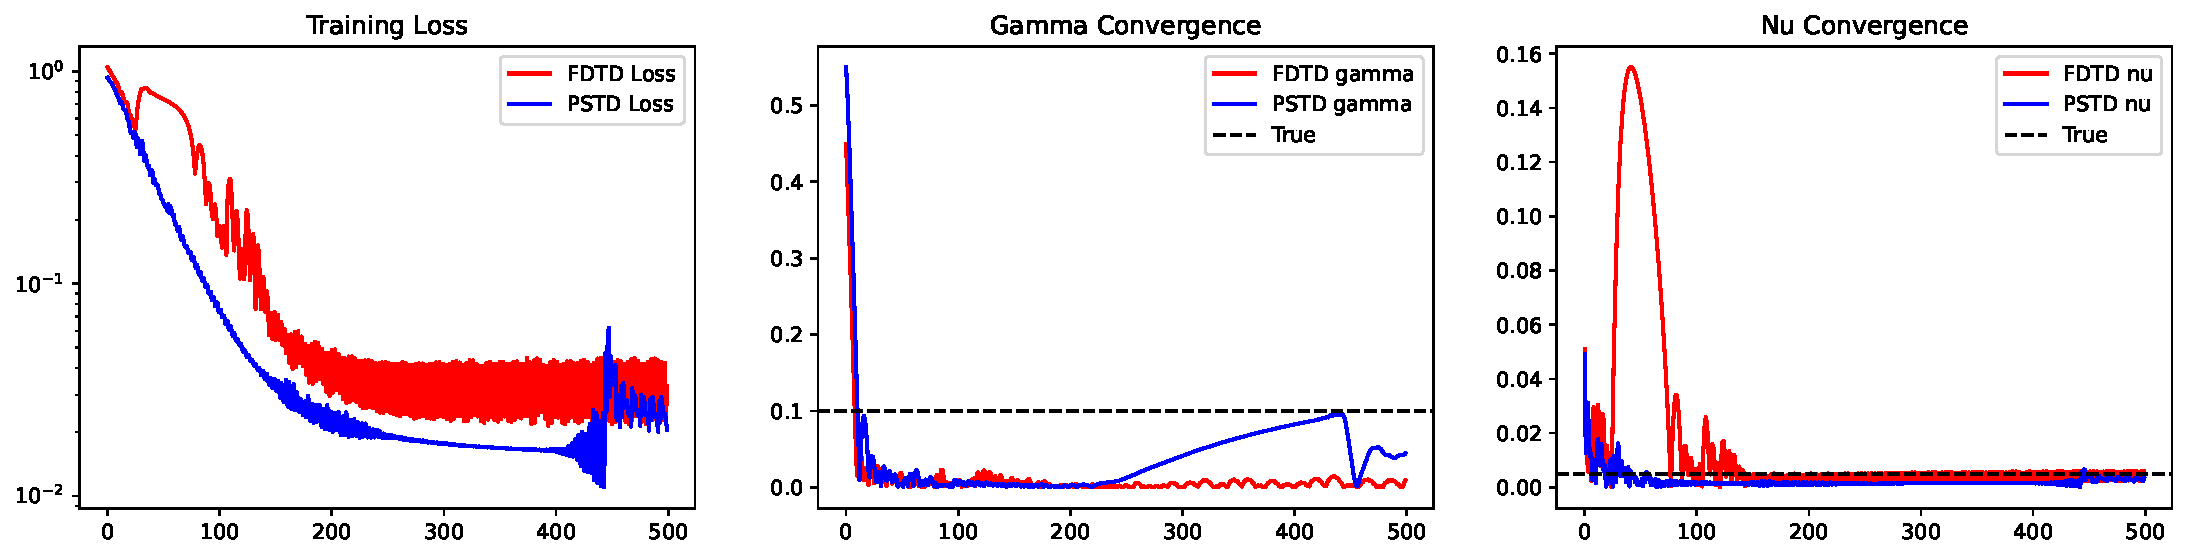
\includegraphics[width=\textwidth]{Images/dpnn/0_StandingWaves_metrics.pdf}
    \caption{Experiment 1 (Standing Waves): Convergence of the composite loss function and the estimated physical damping parameters ($\gamma, \nu$) for the FDTD and PSTD differentiable solvers.}
    \label{fig:0_metrics}
\end{figure}
\vspace{-1cm}
\begin{figure}[H]
    \centering
    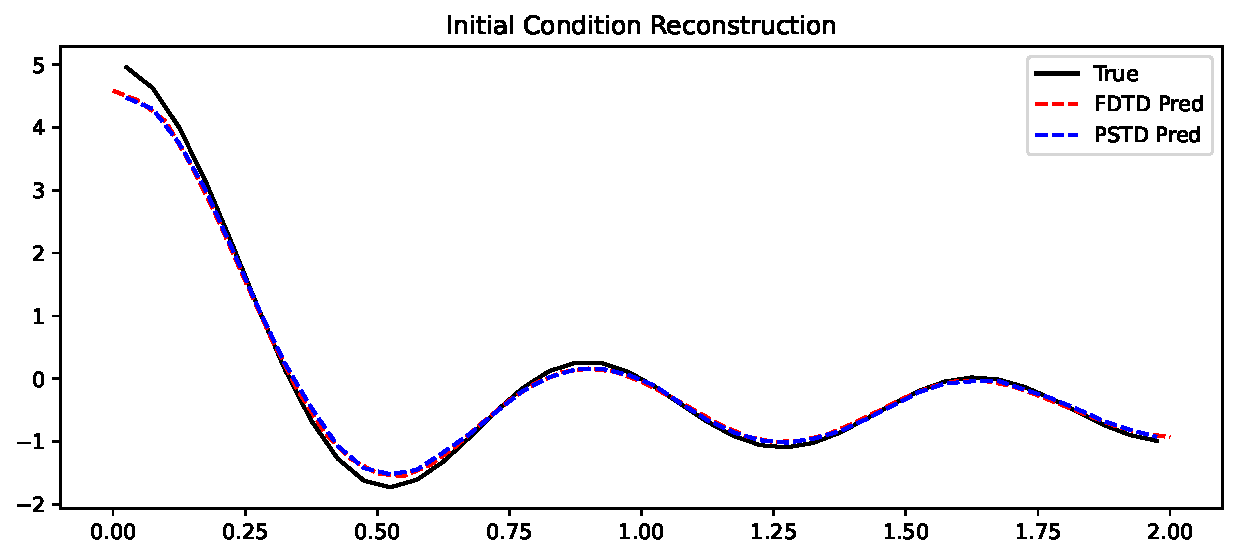
\includegraphics[width=0.6\textwidth]{Images/dpnn/0_StandingWaves_u0_recon.pdf}
    \caption{Experiment 1 (Standing Waves): Reconstructed initial pressure field $p_0(x)$.}
    \label{fig:0_u0}
\end{figure}
\vspace{-1cm}
\begin{figure}[H]
    \centering
    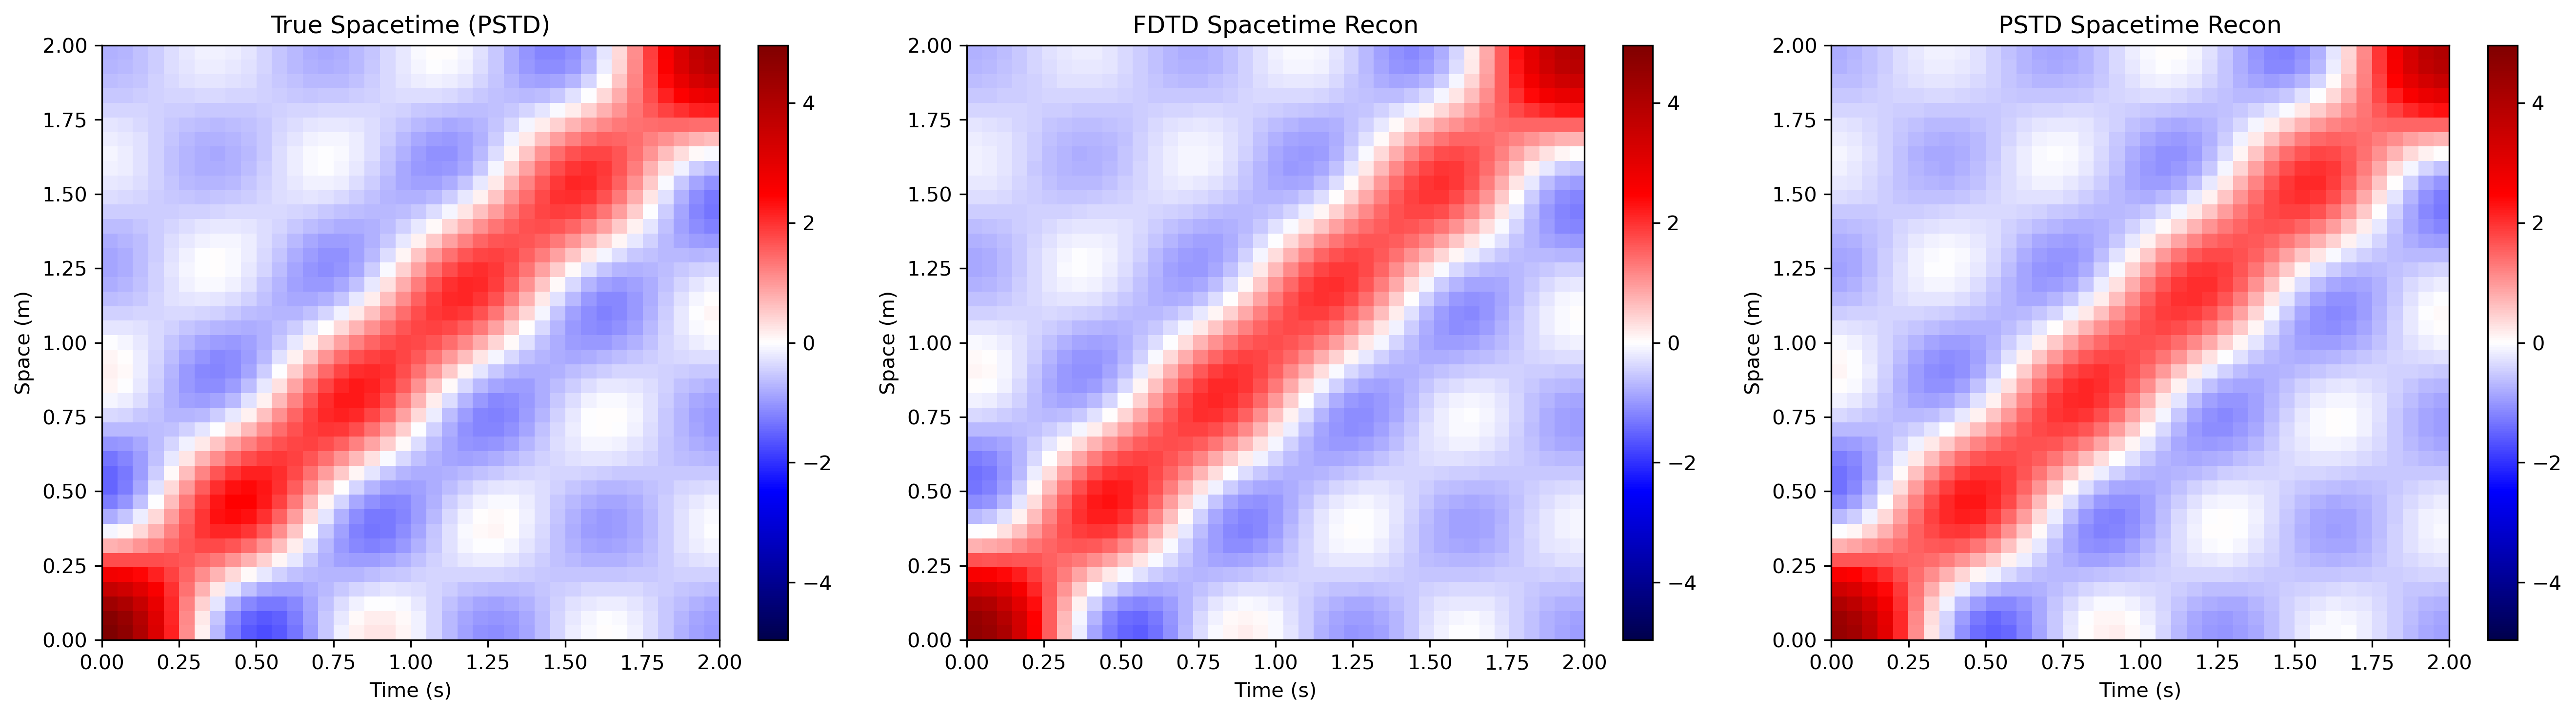
\includegraphics[width=\textwidth]{Images/dpnn/0_StandingWaves_spacetime.png}
    \caption{Experiment 1 (Standing Waves): Spacetime heatmaps comparing the true wave propagation against the FDTD and PSTD reconstructions.}
    \label{fig:0_spacetime}
\end{figure}

\newpage
\subsubsection{Experiment 2: Smooth Pulses}
The smooth pulse initial condition introduces spatial sparsity, activating the $L_1$ regularization. The results (Figures~\ref{fig:1_metrics} to~\ref{fig:1_spacetime}) show that the combination of sparsity and Sobolev smoothness elegantly prevents spurious ringing in the void regions, allowing the neural network to strictly localize the energy of the pulses. The two methods perform equally well.
\begin{figure}[H]
    \centering
    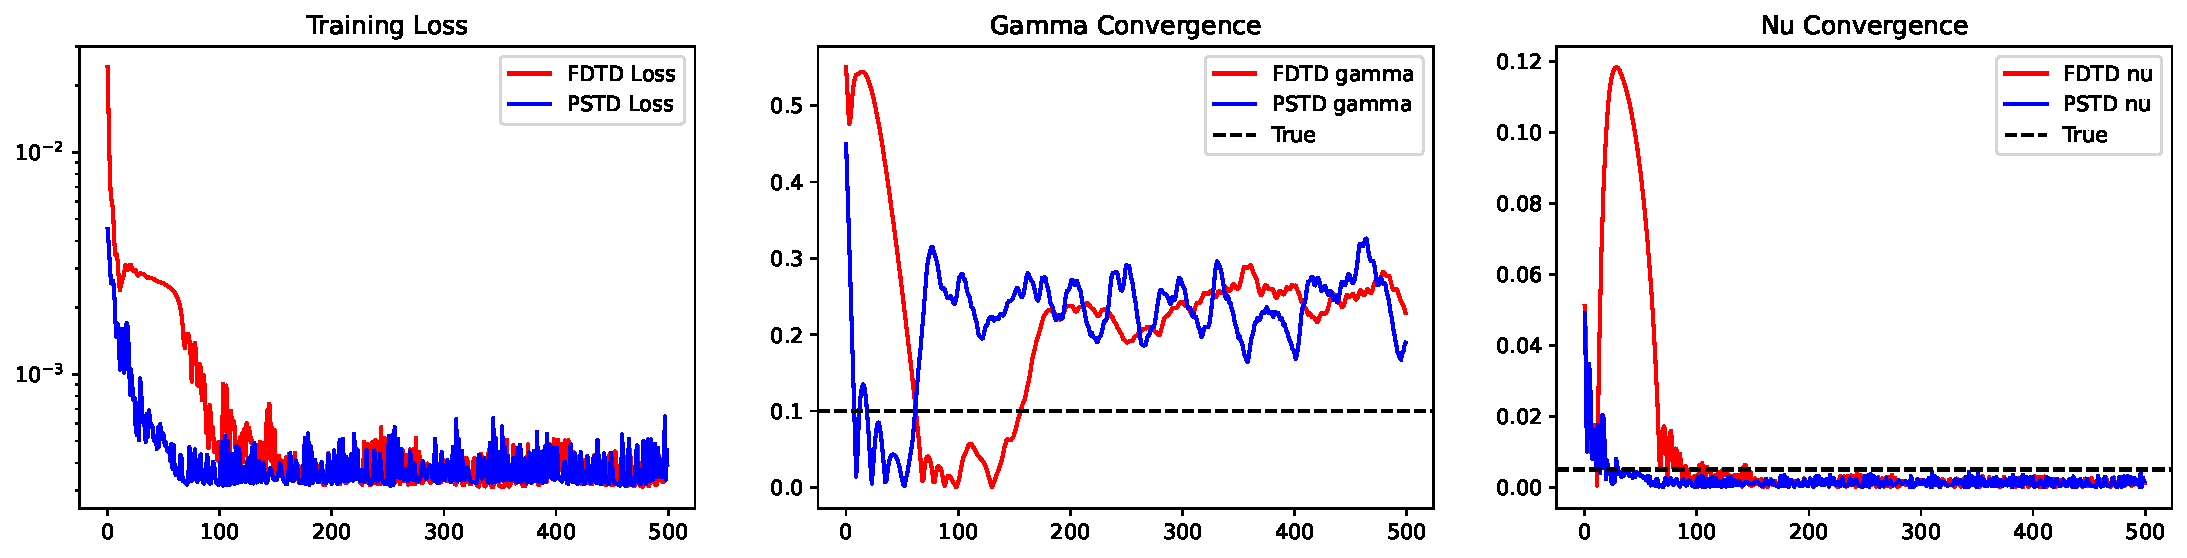
\includegraphics[width=\textwidth]{Images/dpnn/1_Smooth_metrics.pdf}
    \caption{Experiment 2 (Smooth Pulses): Convergence metrics for the network loss and the physical attenuation parameters.}
    \label{fig:1_metrics}
\end{figure}
\vspace{-1cm}
\begin{figure}[H]
    \centering
    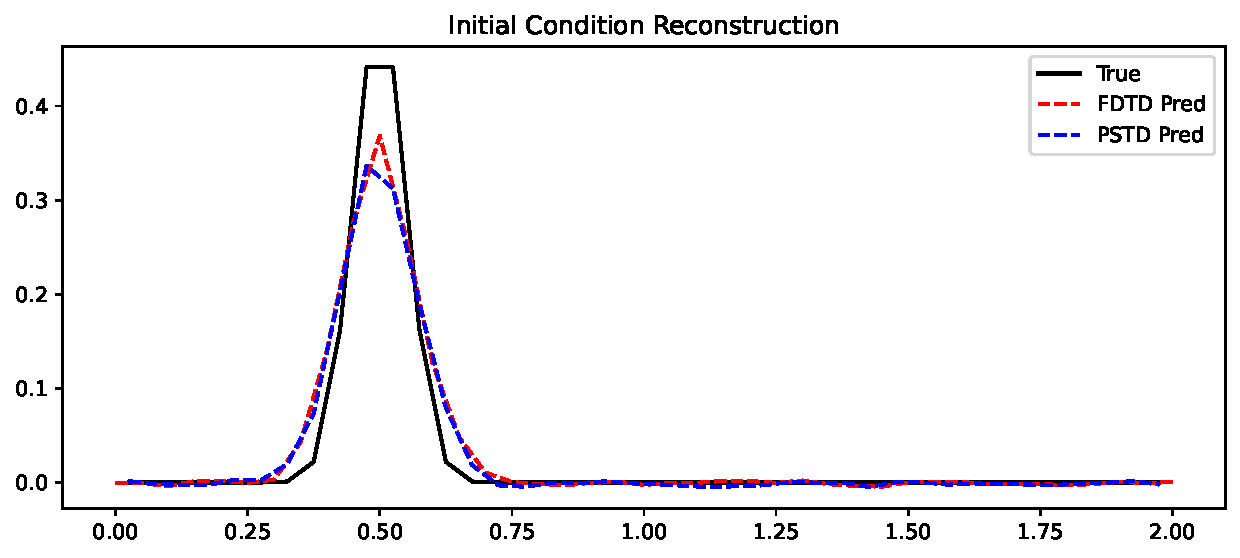
\includegraphics[width=0.6\textwidth]{Images/dpnn/1_Smooth_u0_recon.pdf}
    \caption{Experiment 2 (Smooth Pulses): Reconstructed initial pressure field $p_0(x)$. The void regions are successfully suppressed by the $L_1$ sparsity penalty.}
    \label{fig:1_u0}
\end{figure}
\vspace{-1cm}
\begin{figure}[H]
    \centering
    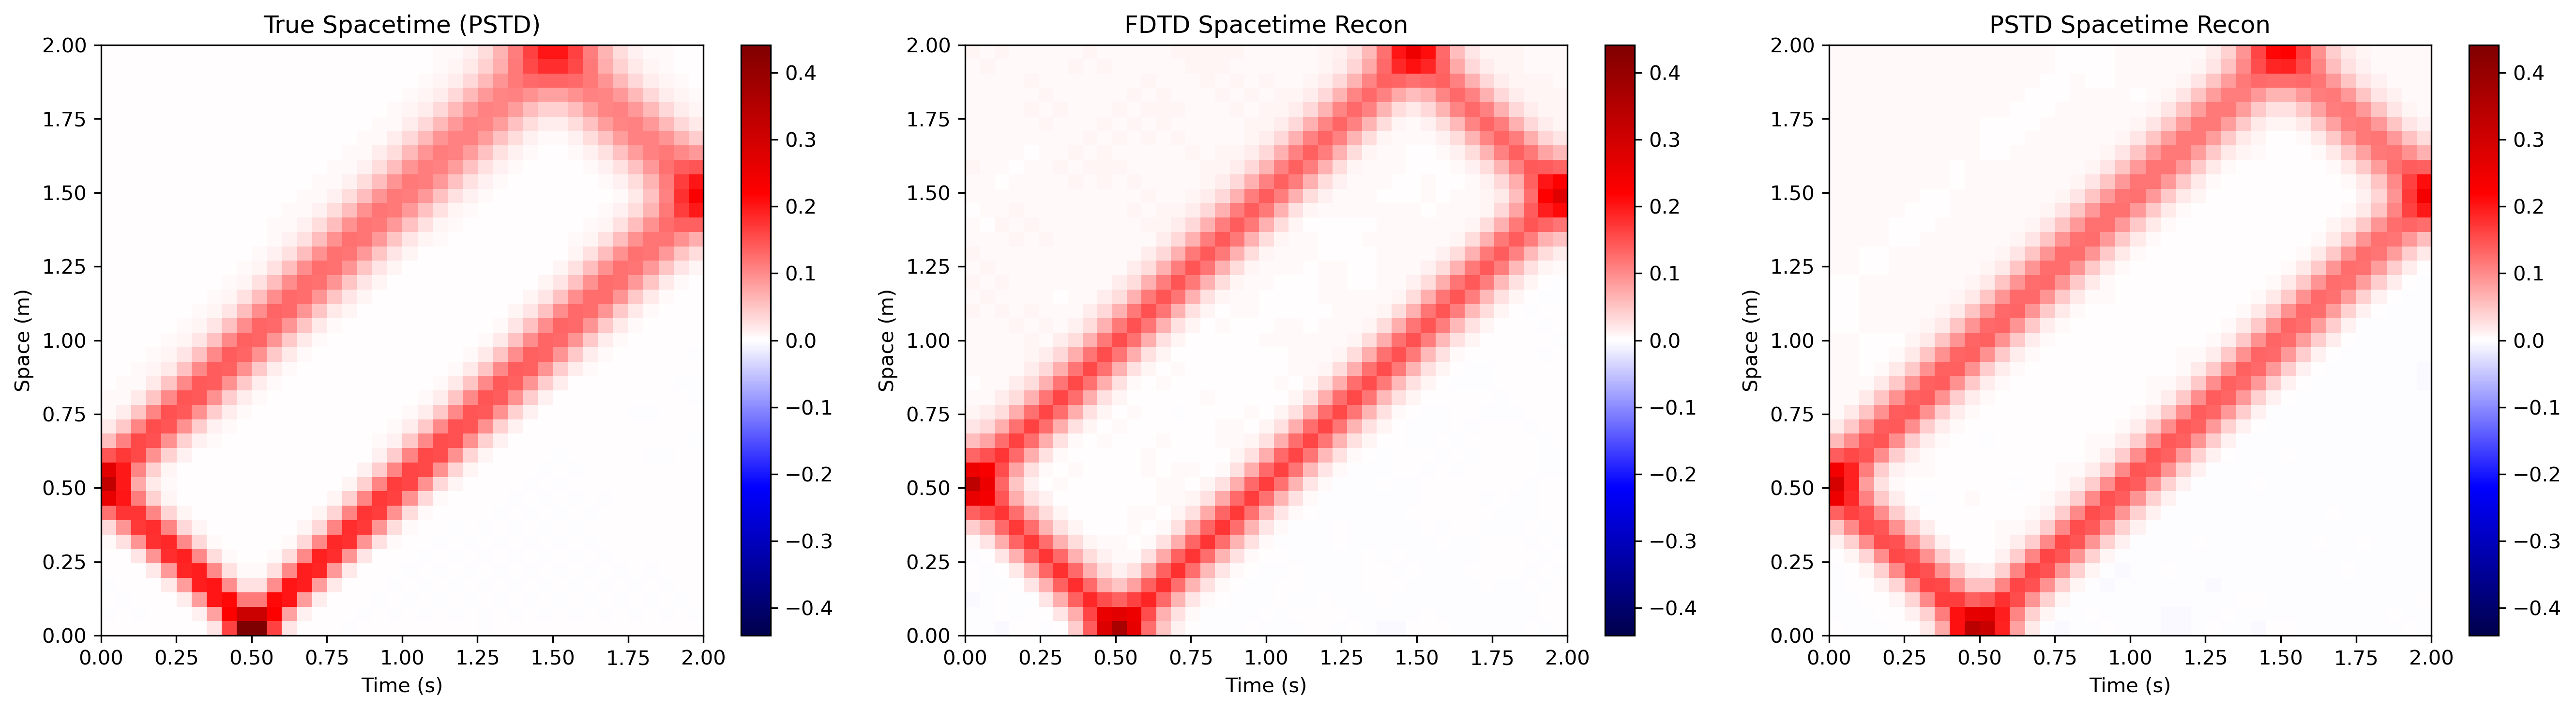
\includegraphics[width=\textwidth]{Images/dpnn/1_Smooth_spacetime.png}
    \caption{Experiment 2 (Smooth Pulses): Spacetime propagation heatmaps. Notice the superior amplitude preservation in the PSTD reconstruction.}
    \label{fig:1_spacetime}
\end{figure}

\newpage
\subsubsection{Experiment 3: Triangle Pulses (Non-smooth)}
The final experiment pushes the DPNN framework to its limits by forcing the SIREN network, an inherently infinitely differentiable ($C^\infty$) function, to fit a $C^0$ non-smooth initial condition. Figures~\ref{fig:2_metrics} to~\ref{fig:2_spacetime} showcase the remarkable robustness of the carefully calibrated Sobolev $H^1$ regularization, which helps suppressing unphysical high-frequency hallucinations without over-smoothing the genuine macroscopic sharp edges of the triangle pulses. The PSTD solver's capacity to transport these sharp gradients without numerical dispersion yields a significantly higher fidelity spacetime reconstruction than the standard FDTD approach, which instead shows high-frequency artifacts.
\begin{figure}[H]
    \centering
    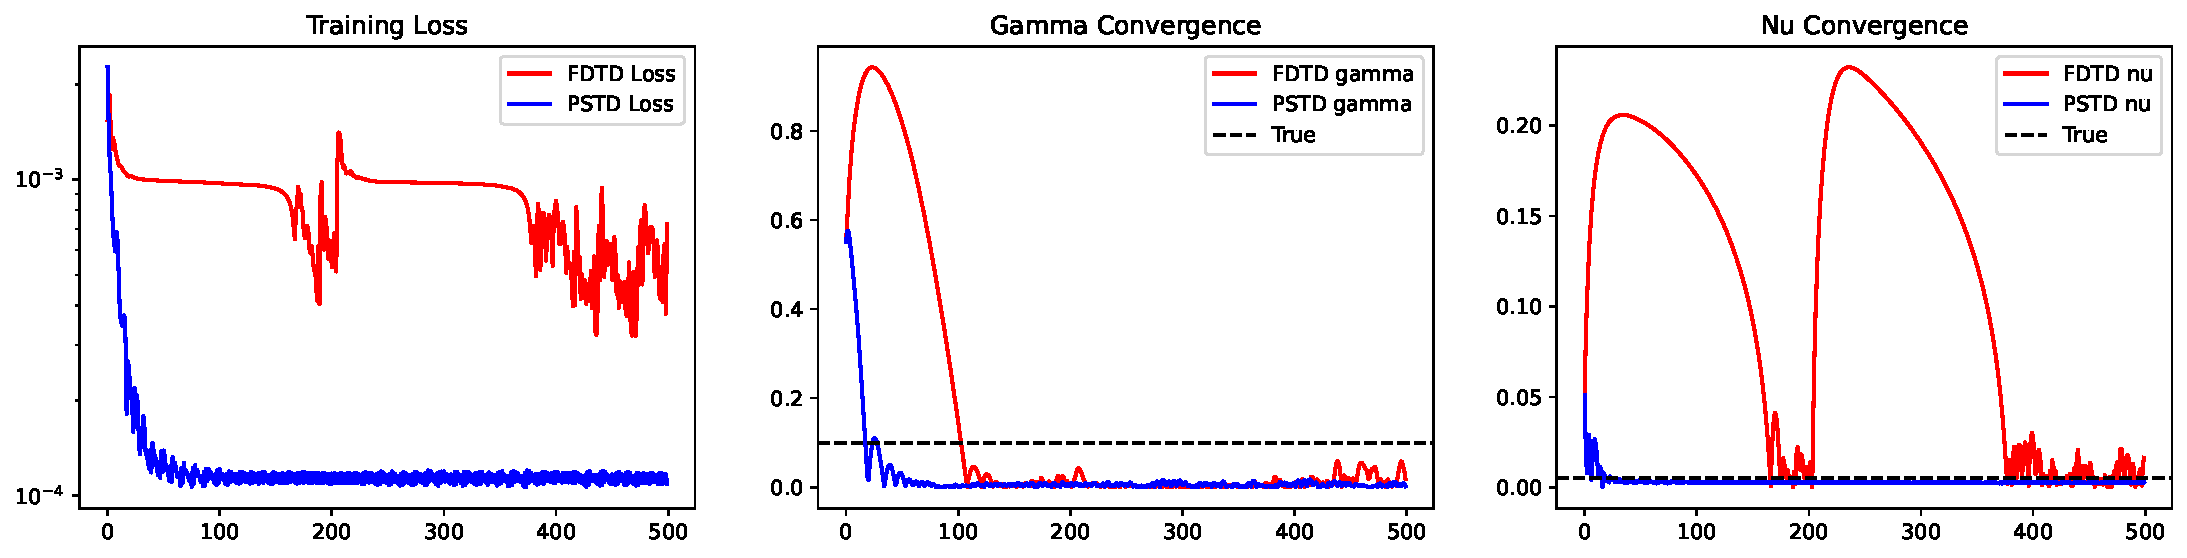
\includegraphics[width=\textwidth]{Images/dpnn/2_Triangle_metrics.pdf}
    \caption{Experiment 3 (Triangle Pulses): Convergence metrics demonstrating stable recovery of the physical parameters even for non-differentiable initial states.}
    \label{fig:2_metrics}
\end{figure}
\vspace{-1cm}
\begin{figure}[H]
    \centering
    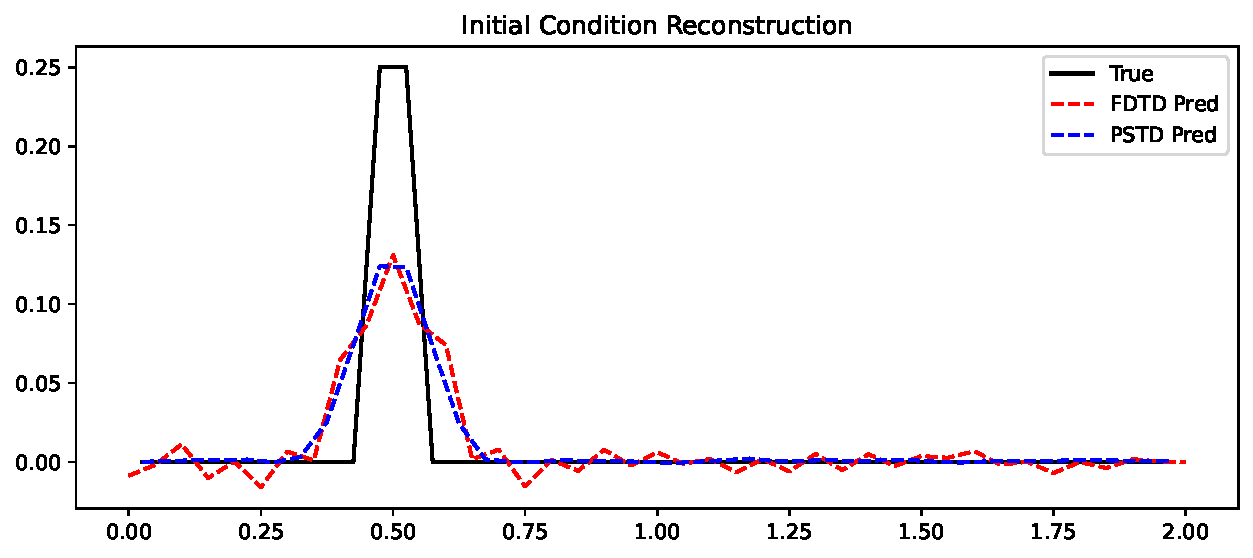
\includegraphics[width=0.6\textwidth]{Images/dpnn/2_Triangle_u0_recon.pdf}
    \caption{Experiment 3 (Triangle Pulses): Reconstructed initial pressure field $p_0(x)$. The SIREN successfully captures the non-smooth peaks without excessive smearing.}
    \label{fig:2_u0}
\end{figure}
\vspace{-1cm}
\begin{figure}[H]
    \centering
    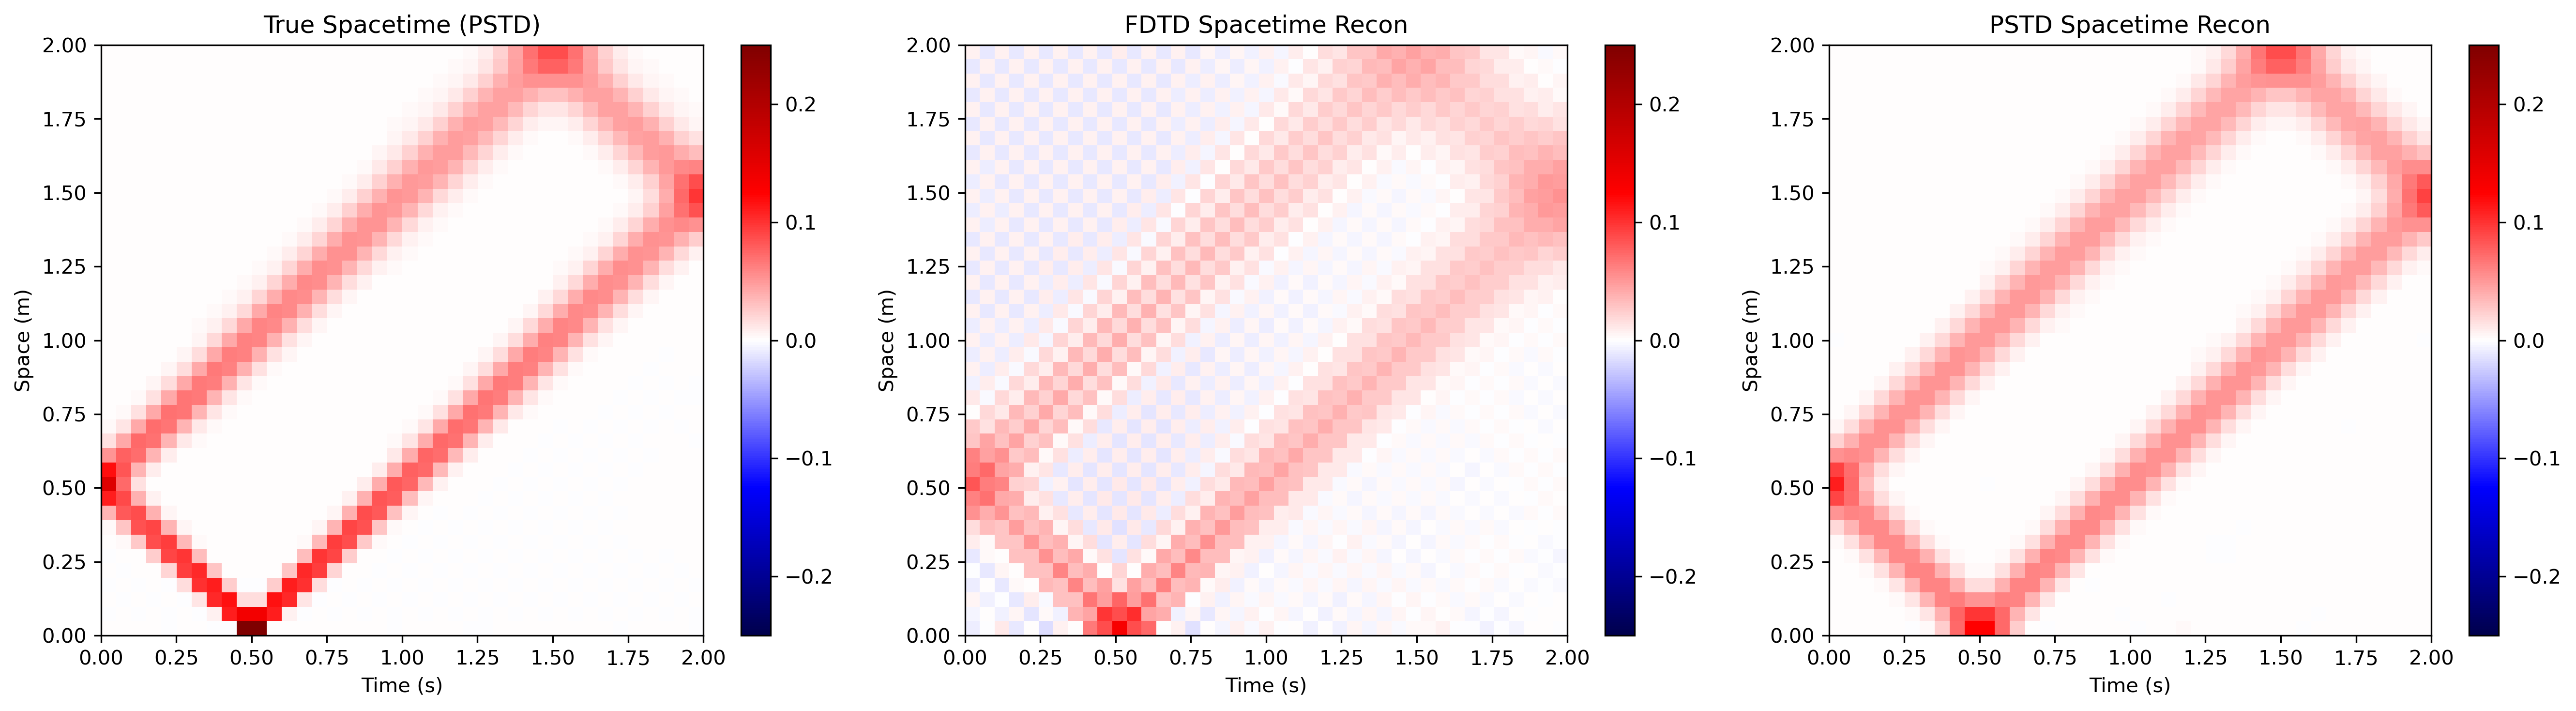
\includegraphics[width=\textwidth]{Images/dpnn/2_Triangle_spacetime.png}
    \caption{Experiment 3 (Triangle Pulses): Spacetime propagation heatmaps emphasizing the PSTD solver's zero-dispersion transport of sharp gradients.}
    \label{fig:2_spacetime}
\end{figure}

\chapter{Conclusion}
\label{ch:conclusion}

This thesis presented a comprehensive suite of numerical and deep learning methods designed to accelerate and invert wave propagation in highly damped viscoelastic media. By systematically addressing the limitations of classical explicit solvers, we introduced novel domain decomposition strategies and leveraged exact modal propagators to achieve unprecedented computational efficiency and spatial accuracy.

The first major contribution of this work was the derivation and analysis of a fully uncoupled Pseudo-Spectral Time Domain (PSTD) solver. By casting the damped wave equation into modal space, we obtained the exact analytic state-transition matrices governing the temporal evolution of the spectral modes. This approach completely eliminated temporal dispersion errors and bypassed the severe stability restrictions traditionally associated with mixed spatial-temporal derivatives, enabling high-fidelity simulations of wave attenuation without the need for implicit global solves.

To scale these methods across distributed computing architectures, we investigated two distinct domain decomposition paradigms. First, we derived the Optimized Schwarz Waveform Relaxation (OSWR) method for the damped wave equation. Through a rigorous continuous min-max analysis, we computed optimal Robin transmission conditions that significantly accelerated the iteration contraction rate compared to classical approaches. Subsequently, we extended the Adaptive Rectangular Decomposition (ARD) method to both FDTD and PSTD frameworks. By replacing traditional interface boundary conditions with a localized, explicit correction operator, we circumvented the need for iterative solvers while maintaining conditional stability. We demonstrated that extending the spatial order of the correction operator yields excellent convergence for smooth wavefields, while properly isolating spectral noise for highly discontinuous profiles.

Finally, we bridged the gap between forward numerical modeling and inverse problem solving by introducing a Differentiable Physics Neural Network (DPNN) architecture. By directly embedding the exact, differentiable PSTD solver into the training loop of a Sinusoidal Representation Network (SIREN), we successfully reconstructed unknown, non-smooth initial pressure fields while jointly recovering the macroscopic physical damping parameters from sparse sensor data. A mathematically rigorously derived Sobolev $H^1$ smoothness penalty gracefully suppressed high-frequency hallucinations without smearing out sharp discontinuities, significantly outperforming purely data-driven black-box inversions.

In conclusion, the integration of pseudo-spectral methods, advanced domain decomposition techniques, and differentiable physics provides a robust, scalable, and highly accurate framework for modeling and reversing complex wave phenomena. Future work will focus on extending these methodologies to higher spatial dimensions, exploring heterogeneous media where modal decomposition becomes coupled, and applying the DPNN architecture to real-world acoustic and medical imaging scenarios.

%-------------------------------------------------------------------------
%	BIBLIOGRAPHY
%-------------------------------------------------------------------------

\addtocontents{toc}{\vspace{2em}} % Add a gap in the Contents, for aesthetics
\bibliography{Thesis_bibliography} % The references information are stored in the file named "Thesis_bibliography.bib"

%-------------------------------------------------------------------------
%	APPENDICES
%-------------------------------------------------------------------------

\cleardoublepage
\addtocontents{toc}{\vspace{2em}} % Add a gap in the Contents, for aesthetics
\appendix
\chapter{Appendix A - Closed-form Expressions of the Modal Propagators}
\label{app:A}

This appendix derives the closed-form expressions of the matrices \(S_m\) and \(T_m\), respectively defined in \eqref{eq:modal_ODE_matrix_S} and \eqref{eq:modal_ODE_matrix_T}, associated with the exact time integration of the modal ordinary differential equations. For convenience, we recall their definitions:
\begin{equation}
S_m=e^{A_m\Delta t},
\end{equation}
\begin{equation}
T_m
=
\int_0^{\Delta t}
e^{A_m(\Delta t-\tau)}
\,d\tau.
\end{equation}

The modal matrix is
\begin{equation}
A_m=
\begin{bmatrix}
0 & 1\\
c^2\lambda_m & -d_m
\end{bmatrix},
\qquad
d_m=\gamma-\nu\lambda_m,
\label{eq:general_A}
\end{equation}
where the Laplace eigenvalues satisfy
\[
\lambda_m\le0.
\]

Whenever \(A_m\) is invertible, Proposition~\ref{prop:Tmatrix} yields
\begin{equation}
T_m
=
A_m^{-1}(S_m-I),
\end{equation}
which considerably simplifies the derivation.

Since the Laplace operator possesses a single zero eigenvalue corresponding to the constant mode, only two fundamentally different situations arise:

\begin{itemize}
\item the constant mode (\(\lambda_m=0\)), for which \(A_m\) is singular and the integral defining \(T_m\) must be evaluated directly;

\item the non-constant modes (\(\lambda_m<0\)), for which \(A_m\) is invertible and the identity \(T_m=A_m^{-1}(S_m-I)\) applies.
\end{itemize}

This classification unifies all damping regimes into only two derivations. Within the non-constant modes, the underdamped, critically damped and overdamped cases are recovered automatically from a single closed-form expression.

\section{Constant mode (\(\lambda_m=0\))}

For the constant mode,
\begin{equation}
\lambda_m=0,
\end{equation}
the modal matrix becomes
\begin{equation}
A_m=
\begin{bmatrix}
0 & 1\\
0 & -d_m
\end{bmatrix},
\end{equation}
which is singular for every value of \(d_m\). Consequently, Proposition~\ref{prop:Tmatrix} cannot be applied and the forcing matrix must be computed directly from its definition.

The powers of \(A_m\) satisfy
\begin{equation}
A_m^n
=
\begin{bmatrix}
0 & (-d_m)^{\,n-1}\\
0 & (-d_m)^n
\end{bmatrix},
\qquad
n\ge1.
\end{equation}

Substituting these expressions into the Taylor expansion of the matrix exponential,
\begin{equation}
e^{A_m\Delta t}
=
I
+
A_m\Delta t
+
\frac{(A_m\Delta t)^2}{2!}
+\cdots,
\end{equation}
yields
\begin{equation}
S_m
=
\begin{bmatrix}
1 &
\displaystyle
\sum_{n=1}^{\infty}
\frac{(-d_m)^{\,n-1}\Delta t^n}{n!}
\\[3ex]
0 &
\displaystyle
\sum_{n=0}^{\infty}
\frac{(-d_m\Delta t)^n}{n!}
\end{bmatrix}.
\end{equation}

Recognizing the exponential series gives
\begin{equation}
\sum_{n=0}^{\infty}
\frac{(-d_m\Delta t)^n}{n!}
=
e^{-d_m\Delta t},
\end{equation}
while
\begin{equation}
\sum_{n=1}^{\infty}
\frac{(-d_m)^{\,n-1}\Delta t^n}{n!}
=
\frac{1-e^{-d_m\Delta t}}{d_m}.
\end{equation}

Therefore,
\begin{equation}
S_m
=
\begin{bmatrix}
1 &
\dfrac{1-e^{-d_m\Delta t}}{d_m}
\\[3ex]
0 &
e^{-d_m\Delta t}
\end{bmatrix},
\label{eq:constantSm}
\end{equation}
where the upper-right entry is understood by continuity when \(d_m=0\).

Indeed,
\begin{equation}
\lim_{d_m\to0}
\frac{1-e^{-d_m\Delta t}}{d_m}
=
\Delta t,
\end{equation}
recovering the undamped constant-mode propagator
\[
S_m=
\begin{bmatrix}
1 & \Delta t\\
0 & 1
\end{bmatrix}.
\]

To derive the forcing matrix, we integrate the matrix exponential directly:
\begin{equation}
T_m
=
\int_0^{\Delta t}
e^{A_ms}\,ds.
\end{equation}

Using \eqref{eq:constantSm} with \(\Delta t\) replaced by \(s\),
\begin{equation}
e^{A_ms}
=
\begin{bmatrix}
1 &
\dfrac{1-e^{-d_ms}}{d_m}
\\[3ex]
0 &
e^{-d_ms}
\end{bmatrix},
\end{equation}
gives
\begin{equation}
T_m
=
\begin{bmatrix}
\Delta t &
\dfrac{e^{-d_m\Delta t}-1+d_m\Delta t}{d_m^2}
\\[3ex]
0 &
\dfrac{1-e^{-d_m\Delta t}}{d_m}
\end{bmatrix}.
\label{eq:constantTm}
\end{equation}

Again, the removable singularity at \(d_m=0\) is resolved by taking the limits
\begin{equation}
\lim_{d_m\to0}
\frac{e^{-d_m\Delta t}-1+d_m\Delta t}{d_m^2}
=
\frac{\Delta t^2}{2}, \quad \lim_{d_m\to0}
\dfrac{1-e^{-d_m\Delta t}}{d_m}
=
\Delta t,
\end{equation}
so that
\[
T_m=
\begin{bmatrix}
\Delta t &
\dfrac{\Delta t^2}{2}
\\
0 &
\Delta t
\end{bmatrix}.
\]

Thus, the undamped constant mode is obtained simply as the limit \(d_m\rightarrow0\), showing that the damped and undamped cases are described by the same closed-form expressions.

\section{Non-constant modes (\(\lambda_m<0\))}

For every non-constant mode,
\begin{equation}
\lambda_m<0,
\end{equation}
the modal matrix
\begin{equation}
A_m=
\begin{bmatrix}
0 & 1\\
c^2\lambda_m & -d_m
\end{bmatrix}
\end{equation}
is invertible, since
\begin{equation}
\det(A_m)
=
-c^2\lambda_m
>
0.
\end{equation}
Therefore, Proposition~\ref{prop:Tmatrix} applies, and the forcing matrix can be recovered once the state transition matrix is known:
\begin{equation}
T_m
=
A_m^{-1}(S_m-I).
\end{equation}

Introduce the shifted matrix
\begin{equation}
B_m
=
A_m+\frac{d_m}{2}I
=
\begin{bmatrix}
\dfrac{d_m}{2} & 1\\
c^2\lambda_m & -\dfrac{d_m}{2}
\end{bmatrix},
\end{equation}
and define the discriminant
\begin{equation}
\delta_m
=
\sqrt{d_m^2+4c^2\lambda_m},
\end{equation}
which may be either real, null or purely imaginary.

A direct computation gives
\begin{align}
B_m^2
&=
\begin{bmatrix}
\dfrac{d_m}{2} & 1\\
c^2\lambda_m & -\dfrac{d_m}{2}
\end{bmatrix}^2
\nonumber\\
&=
\begin{bmatrix}
\dfrac{d_m^2}{4}+c^2\lambda_m & 0\\
0 & \dfrac{d_m^2}{4}+c^2\lambda_m
\end{bmatrix}
\nonumber\\
&=
\frac{\delta_m^2}{4}I.
\label{eq:Bsquare}
\end{align}

Since
\begin{equation}
A_m
=
-\frac{d_m}{2}I+B_m,
\end{equation}
and the identity matrix commutes with every matrix,
\begin{equation}
e^{A_m\Delta t}
=
e^{-d_m\Delta t/2}
e^{B_m\Delta t}.
\end{equation}

The exponential of \(B_m\) is obtained from its Taylor expansion,
\begin{equation}
e^{B_m\Delta t}
=
I
+
B_m\Delta t
+
\frac{(B_m\Delta t)^2}{2!}
+
\frac{(B_m\Delta t)^3}{3!}
+\cdots.
\end{equation}

Using \eqref{eq:Bsquare}, the even powers satisfy
\begin{equation}
B_m^{2k}
=
\left(\frac{\delta_m}{2}\right)^{2k}I,
\end{equation}
while the odd powers satisfy
\begin{equation}
B_m^{2k+1}
=
\left(\frac{\delta_m}{2}\right)^{2k}B_m.
\end{equation}

Separating the Taylor series into even and odd powers yields
\begin{align}
e^{B_m\Delta t}
&=
I
\sum_{k=0}^{\infty}
\frac{\left(\frac{\delta_m\Delta t}{2}\right)^{2k}}
{(2k)!}
\nonumber\\
&\qquad
+
\frac{2B_m}{\delta_m}
\sum_{k=0}^{\infty}
\frac{\left(\frac{\delta_m\Delta t}{2}\right)^{2k+1}}
{(2k+1)!}.
\end{align}

Recognizing the Taylor expansions of the hyperbolic cosine and sine gives
\begin{equation}
e^{B_m\Delta t}
=
\cosh\!\left(
\frac{\delta_m\Delta t}{2}
\right)
I
+
\frac{2\sinh(\delta_m\Delta t/2)}
{\delta_m}
B_m.
\end{equation}

Substituting the definition of \(B_m\) yields the unified expression
\begin{equation}
S_m
=
e^{-d_m\Delta t/2}
\left[
\cosh\!\left(
\frac{\delta_m\Delta t}{2}
\right)
I
+
\frac{2\sinh(\delta_m\Delta t/2)}
{\delta_m}
\left(
A_m+\frac{d_m}{2}I
\right)
\right].
\label{eq:SmUnified}
\end{equation}

Since \(A_m\) is invertible,
\begin{equation}
T_m
=
A_m^{-1}(S_m-I).
\label{eq:TmUnified}
\end{equation}

Equations \eqref{eq:SmUnified} and \eqref{eq:TmUnified} provide a unified expression valid for every non-constant mode. The classical damping regimes follow as particular cases.

\subsection*{Underdamped regime}

When
\begin{equation}
d_m^2+4c^2\lambda_m<0,
\end{equation}
the discriminant is purely imaginary. Writing
\begin{equation}
\delta_m
=
2i\omega_m,
\qquad
\omega_m
=
\frac12
\sqrt{-d_m^2-4c^2\lambda_m},
\end{equation}
and using the identities
\begin{equation}
\cosh(i\theta)=\cos\theta,
\qquad
\sinh(i\theta)=i\sin\theta,
\end{equation}
equation \eqref{eq:SmUnified} becomes
\begin{equation}
S_m
=
e^{-d_m\Delta t/2}
\left[
\cos(\omega_m\Delta t)I
+
\frac{\sin(\omega_m\Delta t)}
{\omega_m}
\left(
A_m+\frac{d_m}{2}I
\right)
\right].
\end{equation}

\subsection*{Critically damped regime}

When
\begin{equation}
d_m^2+4c^2\lambda_m=0,
\end{equation}
we have
\begin{equation}
\delta_m=0.
\end{equation}

Using
\begin{equation}
\lim_{z\to0}
\frac{\sinh z}{z}
=
1,
\end{equation}
equation \eqref{eq:SmUnified} reduces to
\begin{equation}
S_m
=
e^{-d_m\Delta t/2}
\left[
I
+
\Delta t
\left(
A_m+\frac{d_m}{2}I
\right)
\right].
\end{equation}

\subsection*{Overdamped regime}

When
\begin{equation}
d_m^2+4c^2\lambda_m>0,
\end{equation}
the discriminant \(\delta_m\) is real, and equation~\eqref{eq:SmUnified} directly provides the overdamped propagator in terms of hyperbolic functions. No further specialization is required.

\chapter{Appendix B}
It may be necessary to include another appendix to better organize the presentation of supplementary material.


% LIST OF FIGURES
\listoffigures

% LIST OF TABLES
\listoftables

% LIST OF SYMBOLS
% Write out the List of Symbols in this page
\chapter*{List of Symbols} % You have to include a chapter for your list of symbols (
\begin{table}[H]
    \centering
    \begin{tabular}{lll}
        \textbf{Variable} & \textbf{Description} & \textbf{SI unit} \\\hline\\[-9px]
        $\bm{u}$ & solid displacement & m \\[2px]
        $\bm{u}_f$ & fluid displacement & m \\[2px]
    \end{tabular}
\end{table}

% ACKNOWLEDGEMENTS
\chapter*{Acknowledgements}
Here you might want to acknowledge someone.

\cleardoublepage

\end{document}
